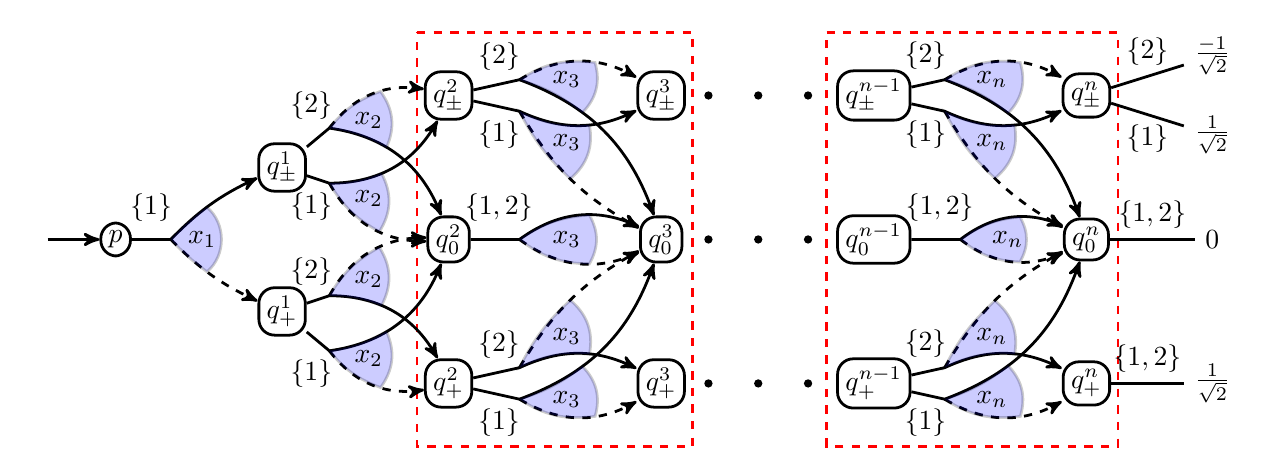
\begin{tikzpicture}[>=stealth',node distance=20mm]
  % coords
  \tikzstyle{hshift}=[xshift=7mm]
  \tikzstyle{aops}=[pos=0.9,below,yshift=0mm,xshift=-2mm]
  \tikzstyle{bops}=[pos=0.9,above,yshift=0mm,xshift=-2mm]
  \tikzstyle{mops}=[pos=0.9,above,yshift=1mm,xshift=-2mm]
  
  \pgfsetlinewidth{1bp}
  \tikzstyle{bddnode}=[draw,rectangle,rounded corners=2mm]
  \tikzstyle{bddleaf}=[]
  \tikzstyle{trans}=[->,>=stealth']
  \tikzstyle{translow}=[->,>=stealth',dashed]
  \tikzstyle{stick}=[-,>=stealth']
  \tikzstyle{ellipsis}=[line width=3pt, line cap=round, dash pattern=on 0pt off 6\pgflinewidth]
  \tikzstyle{hidtrans}=[]
  \tikzstyle{ark}=[]
  \tikzstyle{blueark}=[fill=blue,opacity=0.2]
  \tikzstyle{redark}=[fill=red,opacity=0.6]
  \tikzstyle{redblueark}=[postaction={pattern={Lines[angle=0,distance=1mm,line width=3mm]},
                                      pattern color=blue!20},fill=red!60,line
                                      width=0.2mm]
  \tikzstyle{outp}=[scale=0.75,fill=black!30,inner sep=0.6mm]

  \tikzstyle{bddnodex}=[bddnode,inner sep=1mm]

  % NODES

  \node[bddnodex] (p) {$p$};
  \node[left of=p,xshift=10mm] (root) {};
  \node[bddnodex,below right of=p,hshift,yshift= 5mm] (q1+) {$q^1_+$};
  \node[bddnodex,above right of=p,hshift,yshift=-5mm] (q1+-) {$q^1_\pm$};
  \node[bddnodex,below right of=q1+,hshift,yshift= 5mm] (q2+) {$q^2_+$};
  \node[bddnodex,above right of=q1+,hshift,yshift=-5mm] (q20) {$q^2_0$};
  \node[bddnodex,above right of=q1+-,hshift,yshift=-5mm] (q2+-) {$q^2_\pm$};

  \node[bddnodex,right of=q2+,hshift] (q3+) {$q^3_+$};
  \node[bddnodex,right of=q20,hshift] (q30) {$q^3_0$};
  \node[bddnodex,right of=q2+-,hshift] (q3+-) {$q^3_\pm$};
  \node[bddnodex,right of=q3+,hshift] (qn-1+) {$q^{n-1}_+$};
  \node[bddnodex,right of=q30,hshift] (qn-10) {$q^{n-1}_0$};
  \node[bddnodex,right of=q3+-,hshift] (qn-1+-) {$q^{n-1}_\pm$};
  \node[bddnodex,right of=qn-1+,hshift] (qn+) {$q^{n}_+$};
  \node[bddnodex,right of=qn-10,hshift] (qn0) {$q^{n}_0$};
  \node[bddnodex,right of=qn-1+-,hshift] (qn+-) {$q^{n}_\pm$};
  
  \node[bddleaf, right of=qn+,xshift=-4mm] (r+a) {$\frac{1}{\sqrt{2}}$};
  \node[bddleaf, right of=qn0,xshift=-4mm] (r0a) {$0$};
  \node[bddleaf, right of=qn+-,yshift=-5mm,xshift=-4mm] (r+-a) {$\frac{1}{\sqrt{2}}$};
  \node[bddleaf, right of=qn+-,yshift= 5mm,xshift=-4mm] (r+-b) {$\frac{-1}{\sqrt{2}}$};

  \draw (p) coordinate[yshift=-0mm,xshift=7mm] (pa);
  \draw (q1+) coordinate[yshift=-5mm,xshift=6mm] (q1+a);
  \draw (q1+) coordinate[yshift= 2mm,xshift=6mm] (q1+b);

  \draw (q1+-) coordinate[yshift=-2mm,xshift=6mm] (q1+-a);
  \draw (q1+-) coordinate[yshift= 5mm,xshift=6mm] (q1+-b);

  \draw (q2+) coordinate[yshift=-2mm,xshift=9mm] (q2+a);
  \draw (q2+) coordinate[yshift= 2mm,xshift=9mm] (q2+b);
  \draw (q20) coordinate[yshift=-0mm,xshift=9mm] (q20a);
  \draw (q2+-) coordinate[yshift=-2mm,xshift=9mm] (q2+-a);
  \draw (q2+-) coordinate[yshift= 2mm,xshift=9mm] (q2+-b);

  \draw (qn-1+) coordinate[yshift=-2mm,xshift=9mm] (qn-1+a);
  \draw (qn-1+) coordinate[yshift= 2mm,xshift=9mm] (qn-1+b);
  \draw (qn-10) coordinate[yshift=-0mm,xshift=11mm] (qn-10a);
  \draw (qn-1+-) coordinate[yshift=-2mm,xshift=9mm] (qn-1+-a);
  \draw (qn-1+-) coordinate[yshift= 2mm,xshift=9mm] (qn-1+-b);


  \draw (q3+) coordinate[xshift=6mm] (q3+');
  \draw (q30) coordinate[xshift=6mm] (q30');
  \draw (q3+-) coordinate[xshift=6mm] (q3+-');

  \draw[ellipsis] (q3+') -- (qn-1+);
  \draw[ellipsis] (q30') -- (qn-10);
  \draw[ellipsis] (q3+-') -- (qn-1+-);

  % box
  \draw (q2+-) coordinate[xshift=-4mm,yshift= 8mm] (box11);
  \draw (q3+-) coordinate[xshift= 4mm,yshift= 8mm] (box12);
  \draw (q3+)  coordinate[xshift= 4mm,yshift=-8mm] (box13);
  \draw (q2+)  coordinate[xshift=-4mm,yshift=-8mm] (box14);
  \draw[dashed,red] (box11) to (box12) to (box13) to (box14) to (box11);
  
  \draw (qn-1+-) coordinate[xshift=-6mm,yshift= 8mm] (box11);
  \draw (qn+-) coordinate[xshift= 4mm,yshift= 8mm] (box12);
  \draw (qn+)  coordinate[xshift= 4mm,yshift=-8mm] (box13);
  \draw (qn-1+)  coordinate[xshift=-6mm,yshift=-8mm] (box14);
  \draw[dashed,red] (box11) to (box12) to (box13) to (box14) to (box11);

  %%%%%%%%%%%%%%% transition %%%%%%%%%%%%%%%%%%%
  \draw[translow] (pa)
    to[bend right=10]
    coordinate[pos=0.45] (pa_1)
    (q1+);

  \draw[trans] (p) to 
    node[mops] {$\{1\}$}
    (pa)
    to[bend left=10]
    coordinate[pos=0.45] (pa_2)
    (q1+-);

  \filldraw[blueark] (pa) to[bend right=5] (pa_1) to[bend right=50] (pa_2) to[bend right=5] cycle;
  \node at (pa) [yshift=-0mm,xshift=4mm] {$x_1$};

  %%%%%%%%%%%%%%% transition %%%%%%%%%%%%%%%%%%%
  \draw[translow] (q1+a)
    to[bend right]
    coordinate[pos=0.6] (q1+a_1)
    (q2+);

  \draw[trans] (q1+) to 
    node[aops] {$\{1\}$}
    (q1+a)
    to[bend right]
    coordinate[pos=0.4] (q1+a_2)
    (q20);

  \filldraw[blueark] (q1+a) to[bend right=15] (q1+a_1) to[bend
  right=30] (q1+a_2) to[bend left=10] cycle;
  \node at (q1+a) [yshift=-1mm,xshift=5mm] {$x_2$};

  
  %%%%%%%%%%%%%%% transition %%%%%%%%%%%%%%%%%%%
  \draw[trans] (q1+) to 
    node[bops] {$\{2\}$}
    (q1+b)
    to[bend left]
    coordinate[pos=0.4] (q1+b_1)
    (q2+);

  \draw[translow] (q1+b)
    to[bend left]
    coordinate[pos=0.6] (q1+b_2)
    (q20);

  \filldraw[blueark] (q1+b) to[bend left=10] (q1+b_1) to[bend
  right=30] (q1+b_2) to[bend right=15] cycle;
  \node at (q1+b) [yshift=2mm,xshift=5mm] {$x_2$};

  %%%%%%%%%%%%%%% transition %%%%%%%%%%%%%%%%%%%
  \draw[translow] (q1+-a)
    to[bend right]
    coordinate[pos=0.6] (q1a_1)
    (q20);

  \draw[trans] (q1+-) to 
    node[aops] {$\{1\}$}
    (q1+-a)
    to[bend right]
    coordinate[pos=0.4] (q1a_2)
    (q2+-);

  \filldraw[blueark] (q1+-a) to[bend right=15] (q1a_1) to[bend
  right=30] (q1a_2) to[bend left=10] cycle;
  \node at (q1+-a) [yshift=-2mm,xshift=5mm] {$x_2$};

  %%%%%%%%%%%%%%% transition %%%%%%%%%%%%%%%%%%%
  
  \draw[trans] (q1+-) to 
    node[bops] {$\{2\}$}
    (q1+-b)
    to[bend left]
    coordinate[pos=0.4] (q1b_1)
    (q20);

  \draw[translow] (q1+-b)
    to[bend left]
    coordinate[pos=0.6] (q1b_2)
    (q2+-);

  \filldraw[blueark] (q1+-b) to[bend left=10] (q1b_1) to[bend
  right=30] (q1b_2) to[bend right=15] cycle;
  \node at (q1+-b) [yshift=1mm,xshift=5mm] {$x_2$};

  %%%%%%%%%%%%%%% transition %%%%%%%%%%%%%%%%%%%

  \draw[trans] (q2+) to 
  node[bops] {$\{2\}$}
  (q2+b)
  to[bend left=25]
  coordinate[pos=0.6] (q2+b_2)
  (q3+);

  \draw[translow] (q2+b)
  to[bend left=15]
  coordinate[pos=0.5] (q2+b_1)
  (q30);

  \filldraw[blueark] (q2+b) to[bend left=10] (q2+b_1) to[bend left=30] (q2+b_2) to[bend right=15] cycle;
  \node at (q2+b) [yshift=4mm,xshift=6mm] {$x_3$};
  
  %%%%%%%%%%%%%%% transition %%%%%%%%%%%%%%%%%%%

  \draw[trans] (q2+) to
  node[aops] {$\{1\}$}
  (q2+a)
  to[bend right=25]
  coordinate[pos=0.35] (q2+a_2)
  (q30);

  \draw[translow] (q2+a) 
  to[bend right]
  coordinate[pos=0.65] (q2+a_1)
  (q3+);
  
  \filldraw[blueark] (q2+a) to[bend right=20] (q2+a_1) to[bend right=30] (q2+a_2) to[bend left=10] cycle;
  \node at (q2+a) [yshift=-0mm,xshift=6mm] {$x_3$};

  %%%%%%%%%%%%%%% transition %%%%%%%%%%%%%%%%%%%

  \draw[trans] (q20) to 
  node[mops] {$\{1,2\}$}
  (q20a)
  to[bend left]
  coordinate[pos=0.6] (q20a_2)
  (q30);

  \draw[translow] (q20a) 
  to[bend right]
  coordinate[pos=0.6] (q20a_1)
  (q30);

  \filldraw[blueark] (q20a) to[bend right=18] (q20a_1) to[bend right] (q20a_2) to[bend right=15] cycle;
  \node at (q20a) [xshift=6mm] {$x_3$};
  
  %%%%%%%%%%%%%%% transition %%%%%%%%%%%%%%%%%%%

  \draw[trans] (q2+-) to 
  node[aops] {$\{1\}$}
  (q2+-a)
  to[bend right=25]
  coordinate[pos=0.6] (q2+-a_2)
  (q3+-);

  \draw[translow] (q2+-a)
  to[bend right=15]
  coordinate[pos=0.5] (q2+-a_1)
  (q30);

  \filldraw[blueark] (q2+-a) to[bend right=10] (q2+-a_1) to[bend right=30] (q2+-a_2) to[bend left=15] cycle;
  \node at (q2+-a) [yshift=-4mm,xshift=6mm] {$x_3$};
  
  %%%%%%%%%%%%%%% transition %%%%%%%%%%%%%%%%%%%

  \draw[trans] (q2+-) to
  node[bops] {$\{2\}$}
  (q2+-b)
  to[bend left=25]
  coordinate[pos=0.35] (q2+-b_2)
  (q30);

  \draw[translow] (q2+-b) 
  to[bend left]
  coordinate[pos=0.65] (q2+-b_1)
  (q3+-);
  
  \filldraw[blueark] (q2+-b) to[bend left=20] (q2+-b_1) to[bend left=30] (q2+-b_2) to[bend right=10] cycle;
  \node at (q2+-b) [yshift=-0mm,xshift=6mm] {$x_3$};

  %%%%%%%%%%%%%%% transition %%%%%%%%%%%%%%%%%%%

  %%%%%%%%%%%%%%% transition %%%%%%%%%%%%%%%%%%%

  \draw[trans] (qn-1+) to 
  node[bops] {$\{2\}$}
  (qn-1+b)
  to[bend left=25]
  coordinate[pos=0.6] (qn-1+b_2)
  (qn+);

  \draw[translow] (qn-1+b)
  to[bend left=15]
  coordinate[pos=0.5] (qn-1+b_1)
  (qn0);

  \filldraw[blueark] (qn-1+b) to[bend left=10] (qn-1+b_1) to[bend left=30] (qn-1+b_2) to[bend right=15] cycle;
  \node at (qn-1+b) [yshift=4mm,xshift=6mm] {$x_n$};
  
  %%%%%%%%%%%%%%% transition %%%%%%%%%%%%%%%%%%%

  \draw[trans] (qn-1+) to
  node[aops] {$\{1\}$}
  (qn-1+a)
  to[bend right=25]
  coordinate[pos=0.35] (qn-1+a_2)
  (qn0);

  \draw[translow] (qn-1+a) 
  to[bend right]
  coordinate[pos=0.65] (qn-1+a_1)
  (qn+);
  
  \filldraw[blueark] (qn-1+a) to[bend right=20] (qn-1+a_1) to[bend right=30] (qn-1+a_2) to[bend left=10] cycle;
  \node at (qn-1+a) [yshift=-0mm,xshift=6mm] {$x_n$};

  %%%%%%%%%%%%%%% transition %%%%%%%%%%%%%%%%%%%

  \draw[trans] (qn-10) to 
  node[mops] {$\{1,2\}$}
  (qn-10a)
  to[bend left]
  coordinate[pos=0.6] (qn-10a_2)
  (qn0);

  \draw[translow] (qn-10a) 
  to[bend right]
  coordinate[pos=0.6] (qn-10a_1)
  (qn0);

  \filldraw[blueark] (qn-10a) to[bend right=18] (qn-10a_1) to[bend right] (qn-10a_2) to[bend right=15] cycle;
  \node at (qn-10a) [xshift=6mm] {$x_n$};
  
  %%%%%%%%%%%%%%% transition %%%%%%%%%%%%%%%%%%%

  \draw[trans] (qn-1+-) to 
  node[aops] {$\{1\}$}
  (qn-1+-a)
  to[bend right=25]
  coordinate[pos=0.6] (qn-1+-a_2)
  (qn+-);

  \draw[translow] (qn-1+-a)
  to[bend right=15]
  coordinate[pos=0.5] (qn-1+-a_1)
  (qn0);

  \filldraw[blueark] (qn-1+-a) to[bend right=10] (qn-1+-a_1) to[bend right=30] (qn-1+-a_2) to[bend left=15] cycle;
  \node at (qn-1+-a) [yshift=-4mm,xshift=6mm] {$x_n$};
  
  %%%%%%%%%%%%%%% transition %%%%%%%%%%%%%%%%%%%

  \draw[trans] (qn-1+-) to
  node[bops] {$\{2\}$}
  (qn-1+-b)
  to[bend left=25]
  coordinate[pos=0.35] (qn-1+-b_2)
  (qn0);

  \draw[translow] (qn-1+-b) 
  to[bend left]
  coordinate[pos=0.65] (qn-1+-b_1)
  (qn+-);
  
  \filldraw[blueark] (qn-1+-b) to[bend left=20] (qn-1+-b_1) to[bend left=30] (qn-1+-b_2) to[bend right=10] cycle;
  \node at (qn-1+-b) [yshift=-0mm,xshift=6mm] {$x_n$};

  %%%%%%%%%%%%%%% transition %%%%%%%%%%%%%%%%%%%
  
  \draw[trans] (root) to (p);
  \draw[stick] (qn+) to node[above] {$\{1,2\}$} (r+a);
  \draw[stick] (qn0) to node[above] {$\{1,2\}$} (r0a);
  \draw[stick] (qn+-) to node[below] {$\{1\}$} (r+-a);
  \draw[stick] (qn+-) to node[above] {$\{2\}$} (r+-b);
  
\end{tikzpicture}
% \begin{tikzpicture}[>=stealth',node distance=20mm]
%   % coords
%   \tikzstyle{hshift}=[xshift=7mm]
%   \tikzstyle{aops}=[pos=0.9,below,yshift=0mm,xshift=-2mm]
%   \tikzstyle{bops}=[pos=0.9,above,yshift=0mm,xshift=-2mm]
%   \tikzstyle{mops}=[pos=0.9,above,yshift=1mm,xshift=-2mm]
%   
%   \pgfsetlinewidth{1bp}
%   \tikzstyle{bddnode}=[draw,rectangle,rounded corners=2mm]
%   \tikzstyle{bddleaf}=[]
%   \tikzstyle{trans}=[->,>=stealth']
%   \tikzstyle{translow}=[->,>=stealth',dashed]
%   \tikzstyle{stick}=[-,>=stealth']
%   \tikzstyle{ellipsis}=[line width=3pt, line cap=round, dash pattern=on 0pt off 6\pgflinewidth]
%   \tikzstyle{hidtrans}=[]
%   \tikzstyle{ark}=[]
%   \tikzstyle{blueark}=[fill=blue,opacity=0.2]
%   \tikzstyle{redark}=[fill=red,opacity=0.6]
%   \tikzstyle{outp}=[scale=0.75,fill=black!30,inner sep=0.6mm]
%
%   \tikzstyle{bddnodex}=[bddnode,inner sep=1mm]
%
%   % NODES
%
%   \node[bddnodex] (p) {$p$};
%   \node[left of=p,xshift=10mm] (root) {};
%   \node[bddnodex,below right of=p,hshift,yshift= 5mm] (q1+) {$q^1_+$};
%   \node[bddnodex,above right of=p,hshift,yshift=-5mm] (q1+-) {$q^1_\pm$};
%   \node[bddnodex,below right of=q1+,hshift,yshift= 5mm] (q2+) {$q^2_+$};
%   \node[bddnodex,above right of=q1+,hshift,yshift=-5mm] (q20) {$q^2_0$};
%   \node[bddnodex,above right of=q1+-,hshift,yshift=-5mm] (q2+-) {$q^2_\pm$};
%
%   \node[bddnodex,right of=q2+,hshift] (q3+) {$q^3_+$};
%   \node[bddnodex,right of=q20,hshift] (q30) {$q^3_0$};
%   \node[bddnodex,right of=q2+-,hshift] (q3+-) {$q^3_\pm$};
%   \node[bddnodex,right of=q3+,hshift] (qn-1+) {$q^{n-1}_+$};
%   \node[bddnodex,right of=q30,hshift] (qn-10) {$q^{n-1}_0$};
%   \node[bddnodex,right of=q3+-,hshift] (qn-1+-) {$q^{n-1}_\pm$};
%   \node[bddnodex,right of=qn-1+,hshift] (qn+) {$q^{n}_+$};
%   \node[bddnodex,right of=qn-10,hshift] (qn0) {$q^{n}_0$};
%   \node[bddnodex,right of=qn-1+-,hshift] (qn+-) {$q^{n}_\pm$};
%   
%   \node[bddleaf, right of=qn+,xshift=-4mm] (r+a) {$\frac{1}{\sqrt{2}}$};
%   \node[bddleaf, right of=qn0,xshift=-4mm] (r0a) {$0$};
%   \node[bddleaf, right of=qn+-,yshift=-5mm,xshift=-4mm] (r+-a) {$\frac{1}{\sqrt{2}}$};
%   \node[bddleaf, right of=qn+-,yshift= 5mm,xshift=-4mm] (r+-b) {$\frac{-1}{\sqrt{2}}$};
%
%   \draw (p) coordinate[yshift=-0mm,xshift=7mm] (pa);
%   \draw (q1+) coordinate[yshift=-5mm,xshift=6mm] (q1+a);
%   \draw (q1+) coordinate[yshift= 2mm,xshift=6mm] (q1+b);
%
%   \draw (q1+-) coordinate[yshift=-2mm,xshift=6mm] (q1+-a);
%   \draw (q1+-) coordinate[yshift= 5mm,xshift=6mm] (q1+-b);
%
%   \draw (q2+) coordinate[yshift=-2mm,xshift=9mm] (q2+a);
%   \draw (q2+) coordinate[yshift= 2mm,xshift=9mm] (q2+b);
%   \draw (q20) coordinate[yshift=-0mm,xshift=9mm] (q20a);
%   \draw (q2+-) coordinate[yshift=-2mm,xshift=9mm] (q2+-a);
%   \draw (q2+-) coordinate[yshift= 2mm,xshift=9mm] (q2+-b);
%
%   \draw (qn-1+) coordinate[yshift=-2mm,xshift=9mm] (qn-1+a);
%   \draw (qn-1+) coordinate[yshift= 2mm,xshift=9mm] (qn-1+b);
%   \draw (qn-10) coordinate[yshift=-0mm,xshift=11mm] (qn-10a);
%   \draw (qn-1+-) coordinate[yshift=-2mm,xshift=9mm] (qn-1+-a);
%   \draw (qn-1+-) coordinate[yshift= 2mm,xshift=9mm] (qn-1+-b);
%
%
%   \draw (q3+) coordinate[xshift=6mm] (q3+');
%   \draw (q30) coordinate[xshift=6mm] (q30');
%   \draw (q3+-) coordinate[xshift=6mm] (q3+-');
%
%   \draw[ellipsis] (q3+') -- (qn-1+);
%   \draw[ellipsis] (q30') -- (qn-10);
%   \draw[ellipsis] (q3+-') -- (qn-1+-);
%
%   % box
%   \draw (q2+-) coordinate[xshift=-4mm,yshift= 8mm] (box11);
%   \draw (q3+-) coordinate[xshift= 4mm,yshift= 8mm] (box12);
%   \draw (q3+)  coordinate[xshift= 4mm,yshift=-8mm] (box13);
%   \draw (q2+)  coordinate[xshift=-4mm,yshift=-8mm] (box14);
%   \draw[dashed,red] (box11) to (box12) to (box13) to (box14) to (box11);
%   
%   \draw (qn-1+-) coordinate[xshift=-6mm,yshift= 8mm] (box11);
%   \draw (qn+-) coordinate[xshift= 4mm,yshift= 8mm] (box12);
%   \draw (qn+)  coordinate[xshift= 4mm,yshift=-8mm] (box13);
%   \draw (qn-1+)  coordinate[xshift=-6mm,yshift=-8mm] (box14);
%   \draw[dashed,red] (box11) to (box12) to (box13) to (box14) to (box11);
%
%   %%%%%%%%%%%%%%% transition %%%%%%%%%%%%%%%%%%%
%   \draw[translow] (pa)
%     to[bend right=10]
%     coordinate[pos=0.45] (pa_1)
%     (q1+);
%
%   \draw[trans] (p) to 
%     node[mops] {$\{1\}$}
%     (pa)
%     to[bend left=10]
%     coordinate[pos=0.45] (pa_2)
%     (q1+-);
%
%   \filldraw[blueark] (pa) to[bend right=5] (pa_1) to[bend right=50] (pa_2) to[bend right=5] cycle;
%   \node at (pa) [yshift=-0mm,xshift=4mm] {$x_1$};
%
%   %%%%%%%%%%%%%%% transition %%%%%%%%%%%%%%%%%%%
%   \draw[translow] (q1+a)
%     to[bend right]
%     coordinate[pos=0.6] (q1+a_1)
%     (q2+);
%
%   \draw[trans] (q1+) to 
%     node[aops] {$\{1\}$}
%     (q1+a)
%     to[bend right]
%     coordinate[pos=0.4] (q1+a_2)
%     (q20);
%
%   \filldraw[redark] (q1+a) to[bend right=15] (q1+a_1) to[bend
%   right=30] (q1+a_2) to[bend left=10] cycle;
%   \node at (q1+a) [yshift=-1mm,xshift=5mm] {$x_2$};
%
%   
%   %%%%%%%%%%%%%%% transition %%%%%%%%%%%%%%%%%%%
%   \draw[trans] (q1+) to 
%     node[bops] {$\{2\}$}
%     (q1+b)
%     to[bend left]
%     coordinate[pos=0.4] (q1+b_1)
%     (q2+);
%
%   \draw[translow] (q1+b)
%     to[bend left]
%     coordinate[pos=0.6] (q1+b_2)
%     (q20);
%
%   \filldraw[blueark] (q1+b) to[bend left=10] (q1+b_1) to[bend
%   right=30] (q1+b_2) to[bend right=15] cycle;
%   \node at (q1+b) [yshift=2mm,xshift=5mm] {$x_2$};
%
%   %%%%%%%%%%%%%%% transition %%%%%%%%%%%%%%%%%%%
%   \draw[translow] (q1+-a)
%     to[bend right]
%     coordinate[pos=0.6] (q1a_1)
%     (q20);
%
%   \draw[trans] (q1+-) to 
%     node[aops] {$\{1\}$}
%     (q1+-a)
%     to[bend right]
%     coordinate[pos=0.4] (q1a_2)
%     (q2+-);
%
%   \filldraw[redark] (q1+-a) to[bend right=15] (q1a_1) to[bend
%   right=30] (q1a_2) to[bend left=10] cycle;
%   \node at (q1+-a) [yshift=-2mm,xshift=5mm] {$x_2$};
%
%   %%%%%%%%%%%%%%% transition %%%%%%%%%%%%%%%%%%%
%   
%   \draw[trans] (q1+-) to 
%     node[bops] {$\{2\}$}
%     (q1+-b)
%     to[bend left]
%     coordinate[pos=0.4] (q1b_1)
%     (q20);
%
%   \draw[translow] (q1+-b)
%     to[bend left]
%     coordinate[pos=0.6] (q1b_2)
%     (q2+-);
%
%   \filldraw[blueark] (q1+-b) to[bend left=10] (q1b_1) to[bend
%   right=30] (q1b_2) to[bend right=15] cycle;
%   \node at (q1+-b) [yshift=1mm,xshift=5mm] {$x_2$};
%
%   %%%%%%%%%%%%%%% transition %%%%%%%%%%%%%%%%%%%
%
%   \draw[trans] (q2+) to 
%   node[bops] {$\{2\}$}
%   (q2+b)
%   to[bend left=25]
%   coordinate[pos=0.6] (q2+b_2)
%   (q3+);
%
%   \draw[translow] (q2+b)
%   to[bend left=15]
%   coordinate[pos=0.5] (q2+b_1)
%   (q30);
%
%   \filldraw[blueark] (q2+b) to[bend left=10] (q2+b_1) to[bend left=30] (q2+b_2) to[bend right=15] cycle;
%   \node at (q2+b) [yshift=4mm,xshift=6mm] {$x_3$};
%   
%   %%%%%%%%%%%%%%% transition %%%%%%%%%%%%%%%%%%%
%
%   \draw[trans] (q2+) to
%   node[aops] {$\{1\}$}
%   (q2+a)
%   to[bend right=25]
%   coordinate[pos=0.35] (q2+a_2)
%   (q30);
%
%   \draw[translow] (q2+a) 
%   to[bend right]
%   coordinate[pos=0.65] (q2+a_1)
%   (q3+);
%   
%   \filldraw[blueark] (q2+a) to[bend right=20] (q2+a_1) to[bend right=30] (q2+a_2) to[bend left=10] cycle;
%   \node at (q2+a) [yshift=-0mm,xshift=6mm] {$x_3$};
%
%   %%%%%%%%%%%%%%% transition %%%%%%%%%%%%%%%%%%%
%
%   \draw[trans] (q20) to 
%   node[mops] {$\{1,2\}$}
%   (q20a)
%   to[bend left]
%   coordinate[pos=0.6] (q20a_2)
%   (q30);
%
%   \draw[translow] (q20a) 
%   to[bend right]
%   coordinate[pos=0.6] (q20a_1)
%   (q30);
%
%   \filldraw[blueark] (q20a) to[bend right=18] (q20a_1) to[bend right] (q20a_2) to[bend right=15] cycle;
%   \node at (q20a) [xshift=6mm] {$x_3$};
%   
%   %%%%%%%%%%%%%%% transition %%%%%%%%%%%%%%%%%%%
%
%   \draw[trans] (q2+-) to 
%   node[aops] {$\{1\}$}
%   (q2+-a)
%   to[bend right=25]
%   coordinate[pos=0.6] (q2+-a_2)
%   (q3+-);
%
%   \draw[translow] (q2+-a)
%   to[bend right=15]
%   coordinate[pos=0.5] (q2+-a_1)
%   (q30);
%
%   \filldraw[blueark] (q2+-a) to[bend right=10] (q2+-a_1) to[bend right=30] (q2+-a_2) to[bend left=15] cycle;
%   \node at (q2+-a) [yshift=-4mm,xshift=6mm] {$x_3$};
%   
%   %%%%%%%%%%%%%%% transition %%%%%%%%%%%%%%%%%%%
%
%   \draw[trans] (q2+-) to
%   node[bops] {$\{2\}$}
%   (q2+-b)
%   to[bend left=25]
%   coordinate[pos=0.35] (q2+-b_2)
%   (q30);
%
%   \draw[translow] (q2+-b) 
%   to[bend left]
%   coordinate[pos=0.65] (q2+-b_1)
%   (q3+-);
%   
%   \filldraw[blueark] (q2+-b) to[bend left=20] (q2+-b_1) to[bend left=30] (q2+-b_2) to[bend right=10] cycle;
%   \node at (q2+-b) [yshift=-0mm,xshift=6mm] {$x_3$};
%
%   %%%%%%%%%%%%%%% transition %%%%%%%%%%%%%%%%%%%
%
%   %%%%%%%%%%%%%%% transition %%%%%%%%%%%%%%%%%%%
%
%   \draw[trans] (qn-1+) to 
%   node[bops] {$\{2\}$}
%   (qn-1+b)
%   to[bend left=25]
%   coordinate[pos=0.6] (qn-1+b_2)
%   (qn+);
%
%   \draw[translow] (qn-1+b)
%   to[bend left=15]
%   coordinate[pos=0.5] (qn-1+b_1)
%   (qn0);
%
%   \filldraw[blueark] (qn-1+b) to[bend left=10] (qn-1+b_1) to[bend left=30] (qn-1+b_2) to[bend right=15] cycle;
%   \node at (qn-1+b) [yshift=4mm,xshift=6mm] {$x_n$};
%   
%   %%%%%%%%%%%%%%% transition %%%%%%%%%%%%%%%%%%%
%
%   \draw[trans] (qn-1+) to
%   node[aops] {$\{1\}$}
%   (qn-1+a)
%   to[bend right=25]
%   coordinate[pos=0.35] (qn-1+a_2)
%   (qn0);
%
%   \draw[translow] (qn-1+a) 
%   to[bend right]
%   coordinate[pos=0.65] (qn-1+a_1)
%   (qn+);
%   
%   \filldraw[blueark] (qn-1+a) to[bend right=20] (qn-1+a_1) to[bend right=30] (qn-1+a_2) to[bend left=10] cycle;
%   \node at (qn-1+a) [yshift=-0mm,xshift=6mm] {$x_n$};
%
%   %%%%%%%%%%%%%%% transition %%%%%%%%%%%%%%%%%%%
%
%   \draw[trans] (qn-10) to 
%   node[mops] {$\{1,2\}$}
%   (qn-10a)
%   to[bend left]
%   coordinate[pos=0.6] (qn-10a_2)
%   (qn0);
%
%   \draw[translow] (qn-10a) 
%   to[bend right]
%   coordinate[pos=0.6] (qn-10a_1)
%   (qn0);
%
%   \filldraw[blueark] (qn-10a) to[bend right=18] (qn-10a_1) to[bend right] (qn-10a_2) to[bend right=15] cycle;
%   \node at (qn-10a) [xshift=6mm] {$x_n$};
%   
%   %%%%%%%%%%%%%%% transition %%%%%%%%%%%%%%%%%%%
%
%   \draw[trans] (qn-1+-) to 
%   node[aops] {$\{1\}$}
%   (qn-1+-a)
%   to[bend right=25]
%   coordinate[pos=0.6] (qn-1+-a_2)
%   (qn+-);
%
%   \draw[translow] (qn-1+-a)
%   to[bend right=15]
%   coordinate[pos=0.5] (qn-1+-a_1)
%   (qn0);
%
%   \filldraw[blueark] (qn-1+-a) to[bend right=10] (qn-1+-a_1) to[bend right=30] (qn-1+-a_2) to[bend left=15] cycle;
%   \node at (qn-1+-a) [yshift=-4mm,xshift=6mm] {$x_n$};
%   
%   %%%%%%%%%%%%%%% transition %%%%%%%%%%%%%%%%%%%
%
%   \draw[trans] (qn-1+-) to
%   node[bops] {$\{2\}$}
%   (qn-1+-b)
%   to[bend left=25]
%   coordinate[pos=0.35] (qn-1+-b_2)
%   (qn0);
%
%   \draw[translow] (qn-1+-b) 
%   to[bend left]
%   coordinate[pos=0.65] (qn-1+-b_1)
%   (qn+-);
%   
%   \filldraw[blueark] (qn-1+-b) to[bend left=20] (qn-1+-b_1) to[bend left=30] (qn-1+-b_2) to[bend right=10] cycle;
%   \node at (qn-1+-b) [yshift=-0mm,xshift=6mm] {$x_n$};
%
%   %%%%%%%%%%%%%%% transition %%%%%%%%%%%%%%%%%%%
%   
%   \draw[trans] (root) to (p);
%   \draw[stick] (qn+) to node[above] {$\{1,2\}$} (r+a);
%   \draw[stick] (qn0) to node[above] {$\{1,2\}$} (r0a);
%   \draw[stick] (qn+-) to node[below] {$\{1\}$} (r+-a);
%   \draw[stick] (qn+-) to node[above] {$\{2\}$} (r+-b);
%   
% \end{tikzpicture}





%%%%%%%%5%%%%%%%%5%%%%%%%%5%%%%%%%%5%%%%%%%%5%%%%%%%%5%%%%%%%%5%%%%%%%%5%%%%%%%%5

% \documentclass[acmsmall,screen,review]{acmart}
% \documentclass[acmsmall,screen,review,anonymous,nonacm]{acmart}
% \documentclass[acmsmall,screen]{acmart}
\documentclass[acmsmall]{acmart}

\usepackage{graphicx} % Required for inserting images
\usepackage{subcaption} %% For complex figures with \usepackage{tikz}
\usepackage{booktabs,tabularx}
\usepackage{ifthen}
\usepackage{tabularx}
\usepackage{colortbl}
\usepackage{amsmath}
\usepackage{amsthm}
\usepackage{mathtools}
\usepackage{amsfonts}
\usepackage{wrapfig}
\usepackage{paralist}
\usepackage{quantikz}
\usepackage{xspace}
\usepackage{trimclip}   % for clipbox
\usepackage[capitalise]{cleveref}
\usepackage{tikz}
\usepackage{stmaryrd}
\setlength {\marginparwidth }{2cm} 
\usepackage{todonotes}
\usepackage{multicol}
\usepackage{forest}
\usepackage[ruled, vlined, linesnumbered]{algorithm2e}
\usepackage{multirow}
\usepackage{thmtools}
\usepackage{thm-restate}
\usepackage{soul}
\usepackage{framed}
\usepackage{braket}
\usetikzlibrary{arrows}
\usetikzlibrary{positioning}
\usetikzlibrary{cd}
\usetikzlibrary{patterns.meta}
\usepackage{microtype}
\newtheorem{theorem}{Theorem}
\newtheorem{corollary}{Corollary}
\newtheorem{lemma}{Lemma}
\usepackage{adjustbox}
\usepackage{wrapfig}
\newcommand{\sfrac}{\genfrac{}{}{}2}
\newcommand{\ssfrac}{\genfrac{}{}{}3}

\usepackage{transparent}
% \usepackage{tikz}
\usetikzlibrary {graphs,quotes}

\usepackage[xcolor,leftbars]{changebar}
\cbcolor{red}
 \nochangebars

% switch for technical report
\newif\ifTR
% uncomment the following to turn to technical report
% \TRtrue

% use
% \ifTR
% blabla
% \else    % this can be omited
% bleble
% \fi

\ifTR
\else
  %\let\proof\killcontents
  %\let\endproof\endkillcontents
\fi
%%%%%%%%%%%%%%%%%%%%%%%%%%%%%%%%%%

\newcounter{claimcounter}
% %\numberwithin{claimcounter}{thm}
\newenvironment{claim}{\refstepcounter{claimcounter}{\medskip\noindent \underline{Claim \theclaimcounter:}}\itshape}{\smallskip}
\crefname{claimcounter}{Claim}{Claims}
% claims
\newcommand{\claimqed}[0]{\hfill $\blacksquare$}
\newenvironment{claimproof}[1]{\par\noindent\underline{Proof:}\space#1}{\claimqed}
\newenvironment{claimproofnoqed}[1]{\par\noindent\underline{Proof:}\space#1}{}

\Crefname{algocf}{Algorithm}{Algorithms}

%%%%%%%%%%%%%%%%%%%%%%%%%%%%%%%%%%



% \title{Colored Tree Automata and Their Application in Quantum Circuit Verification}
% \title{Synchronized~Tree~Automata~for~Quantum~Circuit~Verification}
% \title{Level-Synchronized Tree Automata for Quantum Circuit Verification}


% \title{Quantum Circuit Verification with Level-Synchronized Tree~Automata}

\ifTR
\title[Verifying Quantum Circuits with Level-Synchronized Tree Automata (Technical Report)]
{Verifying Quantum Circuits with\\
Level-Synchronized Tree Automata (Technical Report)}
\else
\title[Verifying~Quantum~Circuits~with~Level-Synchronized~Tree~Automata]
% {\scalebox{.89}{Verifying~Quantum~Circuits~with~Level-Synchronized~Tree~Automata}}
% {Verifying Quantum Circuits with\\Level-Synchronized Tree Automata}
% {Verifying\,Quantum\,Circuits\,with\,Level-Synchronized\,Tree\,Automata}
% {Verifying Quantum Circuits with Level-Synchronized Tree Automata}
{Verifying Quantum Circuits with Level-Synchronized\\Tree Automata}
% {VerifyingQuantumCircuitswithLevel-SynchronizedTreeAutomata}
\fi

% \title{Verifying Quantum Circuits with Level-Synchronized Tree Automata}

\author{Parosh Aziz Abdulla}
\orcid{0000-0001-6832-6611}
\affiliation{%
  \institution{Uppsala University}
  \city{Uppsala}
  \country{Sweden}
}
\email{parosh@it.uu.se}

\author{Yo-Ga Chen}
\orcid{0009-0003-0498-7287}
\affiliation{%
  \institution{Academia Sinica}
  \city{Taipei}
  \country{Taiwan}
}
\email{googagagaga@gmail.com}

\author{Yu-Fang Chen}
\orcid{0000-0003-2872-0336}
\affiliation{%
  \institution{Academia Sinica}
  \city{Taipei}
  \country{Taiwan}
}
\email{gulu0724@gmail.com}

\author{Lukáš Holík}
\orcid{0000-0001-6957-1651}
\affiliation{%
  \institution{Brno University of Technology}
  \city{Brno}
  \country{Czechia}
}
\affiliation{%
  \institution{Aalborg University}
  \city{Aalborg}
  \country{Denmark}
}
\email{holik@fit.vutbr.cz}

\author{Ondřej Lengál}
\orcid{0000-0002-3038-5875}
\affiliation{%
  \institution{Brno University of Technology}
  \city{Brno}
  \country{Czechia}
}
\email{lengal@fit.vutbr.cz}

\author{Jyun-Ao Lin}
\orcid{0000-0001-8560-2147}
\affiliation{%
  \institution{National Taipei University of Technology}
  \city{Taipei}
  \country{Taiwan}
}
\email{jalin@ntut.edu.tw}

\author{Fang-Yi Lo}
\orcid{0009-0000-4495-6539}
\affiliation{%
  \institution{Academia Sinica}
  \city{Taipei}
  \country{Taiwan}
}
\email{lofangyi@gmail.com}

\author{Wei-Lun Tsai}
\orcid{0009-0003-5832-0867}
\affiliation{%
  \institution{Academia Sinica}
  \city{Taipei}
  \country{Taiwan}
}
\email{alan23273850@gmail.com}

%  \author{Parosh Aziz Abdulla} 
%      \orcid{0000-0001-6832-6611}             %% \orcid is optional
%      \affiliation{ 
%        \institution{Uppsala University}
%        \department{Department of Information Technology}
%        \country{Sweden}
%      }
%      \email{parosh@it.uu.se}
%
%  \author{Yo-Ga Chen} 
%      \orcid{0009-0003-0498-7287}             %% \orcid is optional
%      \affiliation{ 
%        \institution{Academia Sinica}
%        \department{Institute of Information Science}
%        \country{Taiwan}
%      }
%      \email{youchiachen@iis.sinica.edu.tw}
%
%  \author{Yu-Fang Chen} 
%      \orcid{0000-0003-2872-0336}             %% \orcid is optional
%      \affiliation{ 
%        \institution{Academia Sinica}
%        \department{Institute of Information Science}
%        \country{Taiwan}
%      }
%      \email{yfc@iis.sinica.edu.tw}
%
%      
%  \author{Lukáš Holík} 
%      \orcid{0000-0001-6957-1651}             %% \orcid is optional
%      \affiliation{ 
%        \department{The Technical Faculty of IT and Design}             %% \department is recommended
%        \institution{Aalborg University}
%        % \streetaddress{Bo\v{z}et\v{e}chova 2}
%        % \city{Brno}
%        % \postcode{612 00}
%        \country{Denmark}
%      }
%      \email{lukasholik@cs.aau.dk} 
%     \affiliation{ 
%        \department{Faculty of Information Technology}             %% \department is recommended
%        \institution{Brno University of Technology}
%        % \streetaddress{Bo\v{z}et\v{e}chova 2}
%        % \city{Brno}
%        % \postcode{612 00}
%        \country{Czech Republic}
%      }
%
%  \author{Ondřej Lengál} 
%      \orcid{0000-0002-3038-5875}             %% \orcid is optional
%      \affiliation{ 
%        \department{Faculty of Information Technology}             %% \department is recommended
%        \institution{Brno University of Technology}
%        % \streetaddress{Bo\v{z}et\v{e}chova 2}
%        % \city{Brno}
%        % \postcode{612 00}
%        \country{Czech Republic}
%      }
%     \email{lengal@fit.vut.cz}         %% \email is recommended
%
%  \author{Jyun-Ao Lin} 
%      \orcid{0000-0001-8560-2147}
%      \affiliation{ 
%      \department{Innovation Frontier Institute of Research for Science and Technology \& Department of Computer Science and Information Engineering}
%        \institution{National Taipei University of Technology}
%        \country{Taiwan}
%      }
%      \email{jyalin@gmail.com}
%
%  \author{Fang-Yi Lo} 
%      \orcid{0009-0000-4495-6539}             %% \orcid is optional
%      \affiliation{ 
%        \institution{Academia Sinica}
%        \department{Institute of Information Science}
%        \country{Taiwan}
%      }
%     \email{lofangyi@gmail.com}         %% \email is recommended
%
%  \author{Wei-Lun Tsai} 
%  \orcid{0009-0003-5832-0867}
%  \affiliation{ 
%    \institution{Academia Sinica}
%    \department{Institute of Information Science}
%    \country{Taiwan}
%  }
%   \email{alan23273850@gmail.com}
%  \affiliation{ 
%    \institution{National Taiwan University}
%    \department{Graduate Institute of Electronics Engineering}
%    \country{Taiwan}
%  }





\setcopyright{rightsretained}
\acmDOI{10.1145/3704868}
\acmYear{2025}
\acmJournal{PACMPL}
\acmVolume{9}
\acmNumber{POPL}
\acmArticle{32}
\acmMonth{1}
\received{2024-07-11}
\received[accepted]{2024-11-07}

\begin{CCSXML}
<ccs2012>
   <concept>
       <concept_id>10010583.10010786.10010813.10011726</concept_id>
       <concept_desc>Hardware~Quantum computation</concept_desc>
       <concept_significance>500</concept_significance>
       </concept>
   <concept>
       <concept_id>10003752.10003766.10003772</concept_id>
       <concept_desc>Theory of computation~Tree languages</concept_desc>
       <concept_significance>500</concept_significance>
       </concept>
   <concept>
       <concept_id>10011007.10011074.10011099.10011692</concept_id>
       <concept_desc>Software and its engineering~Formal software verification</concept_desc>
       <concept_significance>500</concept_significance>
       </concept>
 </ccs2012>
\end{CCSXML}

\ccsdesc[500]{Hardware~Quantum computation}
\ccsdesc[500]{Theory of computation~Tree languages}
\ccsdesc[500]{Software and its engineering~Formal software verification}


%% Keywords
%% comma separated list
\keywords{quantum circuits, tree automata, verification}  %% \keywords are mandatory in final camera-ready submission


\input{macros.tex}
\input{figs_and_tables.tex}

\begin{document}

%\ol{the title looks more like a git commit message than a title}

\begin{abstract}
We present a new method for the verification of quantum circuits based on
  a novel symbolic representation of sets of quantum states using \emph{level-synchronized tree automata} (\lstas).  
\lstas extend classical tree automata by labeling each transition with a set of
\emph{choices}, which are then used to synchronize subtrees of an accepted tree.
Compared to the traditional tree automata, \lstas have an incomparable expressive
power while maintaining important properties, such as closure under union and
intersection, and decidable language emptiness and inclusion. 
We have developed an efficient and fully automated symbolic verification
algorithm for quantum circuits based on \lstas.
The complexity of supported gate operations is at most quadratic, dramatically
improving the exponential worst-case complexity of an earlier tree automata-based
approach.
Furthermore, we show that \lstas are a promising model for \emph{parameterized verification}, i.e., verifying the correctness of families
of circuits with the same structure for any number of qubits involved, which
principally lies beyond the capabilities of previous automated approaches. 
We implemented this method as a C++ tool and compared it with three symbolic
  quantum circuit verifiers and two simulators on several benchmark examples.
  The results show that our approach can solve problems with sizes orders of
magnitude larger than the state~of~the~art.

%We~demonstrate \lstas' capabilities in parameterized verification by showing thecorrectness of parameterized circuits for GHZ (generalized quantum entanglement),diagonal Hamiltonian simulation, and fermionic unitary evolution, which are frequently used in quantum chemistry and material science. 
%Our method could also solve fixed parameter problems with size orders of magnitude larger than the state of the art.
% magnitude larger than what the state of the art can handle.
%% 
%% We have developed a novel tree automata model, named \emph{colored tree automata} (CTA), that labels each transition with a set of colors. These colors play a crucial role in defining the acceptance condition and enable synchronization between subtrees of an accepted tree. Compared to the traditional tree automata, CTA has an incomparable expressive power and still maintains important properties like being closed under union and intersection, as well as allowing for inclusion and emptiness testing. This new model has significant applications in quantum circuit verification. We have developed an efficient and fully automated symbolic verification algorithm for quantum circuits based on CTA. It is noteworthy that the complexity of supported gate operations is at most quadratic. Furthermore, our new model can be used to handle non-trivial instances of parameterized verification, i.e., verifying the correctness of circuits for any number of qubits involved. We demonstrate CTA's capability in parameterized verification by showing the correctness of a GHZ circuit, a parameterized diagonal Hamiltonian simulation circuit, and circuits for fermionic unitary evolution that are frequently used in quantum chemistry. Our experimental results demonstrate that our algorithm is indeed efficient. We have solved problems with sizes orders of magnitude larger than what the state-of-the-art tool \autoq can handle.
%% 
%  \hide{
%  One important application of colored tree automata is quantum circuit verification. Based on CTA, we have developed an efficient and fully automatic symbolic verification algorithm for quantum circuits. Notably, the complexity of supported gate operations is \emph{at most quadratic}. Furthermore, our new model can be used to handle non-trivial instances of parameterized verification, i.e., verifying the correctness of circuits for any number of involved qubits. For example, we proved the correctness of a GHZ circuit, a parameterized diagonal Hamiltonian simulation circuit, and circuits for fermionic unitary evolution that are often used in quantum chemistry. Experimental results show that our algorithm is indeed efficient. We solve problems with several orders of magnitudes larger than what the state-of-the-art tool \autoq can handle.}    
\end{abstract}
\maketitle

% \renewcommand{\shortauthors}{P.A. Abdulla, Y. Chen, Y. Chen, L. Holík, O. Lengál, J. Lin, F. Lo, W. Tsai}
\renewcommand{\shortauthors}{Parosh Aziz Abdulla,\,Yo-Ga Chen,\,Yu-Fang Chen,\,Lukáš Holík,\,Ondřej Lengál,\,Jyun-Ao Lin,\,Fang-Yi Lo,\,Wei-Lun Tsai}

%%%%%%%%%%%%%%%%%%%%%%%%%%%%%%%%%%%%%%%%%%%%%%%%%%%%%%%%%%%%%%%
\newcommand{\EPRExample}[0]{
 \begin{wrapfigure}[9]{r}{0.25\textwidth}
\vspace{-3mm}
 \begin{quantikz}
  % \lstick{\ketx1\ket{x_1}} & \qw       &\targ{}   & \qw \\
  % \lstick{\ketx2\ket{x_2}} & \gate{H}  &\ctrl{-1}     & \qw
  \lstick{$\ket{x_1}$} & \gate{H}  &\ctrl{1}     & \qw \\
  \lstick{$\ket{x_2}$} & \qw       &\targ{}   & \qw
 \end{quantikz}
 \vspace{-2mm}
 \caption{The Bell state circuit. $\bullet$ denotes the control qubit and $\oplus$
   denotes the target qubit on which $\pauliX$ is applied. }\label{fig:ERPcircuit}

 \end{wrapfigure}
}

%%%%%%%%%%%%%%%%%%%%%%%%%%%%%%%%%%%%%%%%%%%%%%%%
\newcommand{\figNGHZpost}[0]{
\begin{figure}
% \begin{wrapfigure}{r}{1\textwidth}
\centering
\vspace{0cm}

\scalebox{0.7}{
 \input{figs/n-ghz-post.tikz}
}
\caption{An \lsta representing the set of quantum states of the form
 $\frac{1}{\sqrt{2}}(\ket{0b_2b_3\ldots
 b_{n}}\pm\ket{1\bar{b}_2\bar{b}_3\ldots \bar{b}_{n}})$.
 }

\label{fig:nGHZ}
\vspace{-4mm}
% \end{wrapfigure}
\end{figure}}

%%%%%%%%%%%%%%%%%%%%%%%%%%%%%%%%%%%%%%%%%%%%%%%
\newcommand{\figGHZState}[0]{
\begin{wrapfigure}[10]{r}{35mm}
\vspace{-3mm}
%\centering
\scalebox{0.9}{
\input{figs/ghz-state.tikz}
}
\vspace{-7mm}
\caption{GHZ states}
\label{fig:ghz-state-tikz}
\end{wrapfigure}
}


%%%%%%%%%%%%%%%%%%%%%%%%%%%%%%%%%%%%%%%%%%%%%%%%%%%%%%%%%%%%%%%%%%%%%%%%%%%%%%%%
\section{Introduction}\label{sec:intro}
%%%%%%%%%%%%%%%%%%%%%%%%%%%%%%%%%%%%%%%%%%%%%%%%%%%%%%%%%%%%%%%%%%%%%%%%%%%%%%%%


%Quantum computing has emerged as a revolutionary approach capable of tackling computation tasks that are beyond the reach of classical methods. 
%However, computed results are meaningful only when they are correct. Ensuring the correctness of quantum programs is a highly challenging task due to the probabilistic nature of quantum mechanisms. This challenge has produced a pressing need for novel techniques to facilitate reasoning about quantum programs. \emph{Symbolic verification} is one of the most promising approaches, drawing from its success in reasoning about classical programs. Leveraging symbolic verification offers a high level of automation in the verification process. Users are only required to provide minimal annotations for a verification task, with the bulk of the work being handled at the push of a button. 

%Quantum computing is a revolutionary approach that can handle computational tasks beyond the reach of classical methods. However, the results that quantum computing produces are only useful if they are accurate. It is, therefore, crucial to ensure the correctness of quantum programs, but this is extremely difficult due to the probabilistic nature of quantum mechanisms and observation collapses quantum state. To tackle this challenge, novel techniques are needed to help reason about quantum programs. \emph{Symbolic verification}~\cite{rmc,armc,dafny,viper,framac} is among the most promising approaches, and it has been successful in reasoning about classical programs. By leveraging symbolic verification, users can automate the verification process to a high degree. They only need to provide minimal annotations for the verification task, with the bulk of the work being handled automatically at the push of a button.

%Often, we express the \emph{symbolic verification problem} as a triple $\{P\}C\{Q\}$. Here, $P$ and $Q$ are sets of quantum states, and $C$ is a quantum circuit. The problem is to determine if executing $C$ transforms every state in $P$ to a state that is allowed in $Q$. 


%ORIG
%Quantum computing is a technique that can accomplish tasks that are infeasible
%with classical means. For instance, it can factorize integers using a polynomial
%number of instructions, which seems not to be possible using traditional computing
%methods~\cite{Shor94}. Recently, quantum computing has garnered a lot of
%attention owing to the significant progress made in quantum hardware. This
%progress has enabled the achievement of what is known as \emph{quantum
%supremacy}~\cite{AruteABBBBB2019}, which refers to the ability to solve problems
%that would take a state-of-the-art supercomputer thousands of years to solve. As
%quantum computers are likely to play a crucial role in the future, there is
%active development of systems and languages for programming them, for
%example,~\cite{WilleMN19,AltenkirchG05,GreenLRSV13}. Efficient quantum
%algorithms are being developed for solving real-world problems such as machine
%learning~\cite{BiamonteWPRWL17,CilibertoHIPRSW18}, optimization~\cite{Moll18},
%and quantum chemistry~\cite{CaoRO19}.

%Short
%Quantum computing offers unparalleled capabilities by tackling practically insurmountable tasks for classical computers. A prime example is integer factorization, achieved efficiently, a challenge beyond classical methods~\cite{Shor94}. Recent advancements in quantum hardware have led to \emph{quantum supremacy}\cite{AruteABBBBB2019}, marking the ability to solve problems infeasible for even the most advanced supercomputers. As quantum computing emerges as a critical technology for the future, languages and systems are actively developed for programming them~\cite{WilleMN19,AltenkirchG05,GreenLRSV13}.

With the recent progress in quantum hardware and the push to achieve \emph{quantum
supremacy}~(cf., e.g., \cite{AruteABBBBB2019}), the vision of quantum computing, an ability
to solve practical conventionally unsolvable problems, is slowly getting real. 
Systems and languages for programming quantum computers are being intensively
developed~\cite{WilleMN19,AltenkirchG05,GreenLRSV13}, together with efficient quantum
algorithms for solving real-world problems such as machine
learning~\cite{BiamonteWPRWL17,CilibertoHIPRSW18}, optimization~\cite{Moll18},

%Writing quantum programs is immensely challenging due to their probabilistic nature and the exponential size of the computational space. Errors are easy to make and difficult to find. %by traditional means. 
%Tools that aid in reasoning about quantum programs to verify them and detect bugs are in high demand. Ideally, they would be 
%\begin{inparaenum}
%    \item automated,
%    \item fast and scalable,
%    \item supporting specifying properties of interest in a flexible way, and 
%    \item providing precise bug diagnostics.
%\end{inparaenum}

%Tools that aid in reasoning about quantum programs are hence increasingly in demand. 
This progress drives a~demand for tools for reasoning about quantum programs. 
Writing quantum programs is indeed immensely challenging due to their
probabilistic nature and the exponential size of the computational space. Errors
are easily made and difficult to find. %by traditional means. 
Tools for reasoning about quantum programs would ideally have the following
properties:
%
\begin{inparaenum}
    \item \emph{Flexibility:} allows flexible specification of properties of interest,
    \item \emph{Diagnostics:} provides precise bug diagnostics,
    \item \emph{Automation:} operates automatically, and
    \item \emph{Scalability:} scales efficiently to verify useful programs.
\end{inparaenum}

\EPRExample
\emph{Symbolic verification}~\cite{rmc,armc,dafny,viper,framac} is
one of the most successful techniques that satisfies the above criteria for conventional programs.
%Approaches based on symbolic verification are fully automated, flexible in specifying verification properties, provide precise bug reports for diagnostic purposes, and are often capable of handling large-scale programs.
However, there has been minimal progress in the area of symbolic verification for quantum circuits. 
This paper contributes towards filling this gap by adapting automata-based symbolic verification~\cite{rmc} to quantum circuits.
%
More specifically, we think of the symbolic verification problem in terms of Hoare triples
$\hoareof \PreCond C \PostCond$, where $\PreCond$ and $\PostCond$ are sets of quantum states representing the \emph{pre-condition} and the \emph{post-condition}, and $C$ is a
quantum circuit. 
We aim to use symbolic verification to check the \emph{validity} of the triple, ensuring that all executions of $C$ from states in 
$\PreCond$ result in states within $\PostCond$.

\begin{example}\label{ex:hoare_tripple_epr}
As an example of a verification problem, let~$C$ be the circuit creating
Bell states in \cref{fig:ERPcircuit}. The circuit begins by applying the $\hadam$ gate to the first qubit, followed by a controlled-X gate with the first qubit as the control and the second qubit as the target.
The circuit converts 2-qubit computational basis states to Bell states (maximally entangled states). 
Its correct implementation 
satisfies the Hoare triple with the pre-condition $\PreCond=\{\ket{00}, \ket{01},
  \ket{10}, \ket{11}\}$ (computational basis states are denoted using the Dirac notation $\ket{x_1 x_2}$)
  and the post-condition $\PostCond=\{\frac{1}{\sqrt{2}}(\ket{00}\pm\ket{11}),
  \frac{1}{\sqrt{2}}(\ket{01}\pm\ket{10})\mid \pm \in \{+,-\}\}$ (Bell states).
%  \ol{do we really need to define $\pm$ everywhere?}
  % We use Dirac notation $\ket{x_1 x_2}$ to denote quantum states.
%
\qed
\end{example}

%The main challenge in the verification of Hoare triples is the explosion of reachable state spaces of quantum circuits, which is easily exponential in the size of the circuit $C$ and the number of its qubits. 
%\ol{this doesn't seem correct: if I start with the set of $N$ quantum states, I can obtain at most $\#gates$ sets of states, each of the size at most~$N$}
%
%Our answer to this challenge consists of three major components:
%
Our quantum circuit symbolic verification framework comprises three major components:
\begin{inparaenum}
\item a~\emph{succinct symbolic representation of sets of quantum states} allowing efficient manipulation and facilitating flexible specification of desired pre- and post-conditions,
\item algorithms for \emph{symbolic execution of individual quantum gates}, which compute the symbolic representation of output states from input states and explore the reachable state space after circuit execution,
\item \emph{entailment test} on the symbolic representation to verify that all reachable states conform to the specified post-condition or report a witness when the specification is violated.
\end{inparaenum}
Together, these components enable \emph{flexible}, \emph{diagnostic}, \emph{automated}, and \emph{scalable} verification of quantum circuits.

\paragraph{Succinct Symbolic Representation.}

\begin{wrapfigure}[8]{r}{0.23\textwidth}
\centering
\vspace{-0.4cm}
      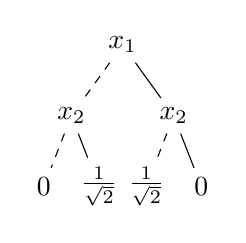
\begin{tikzpicture}
    \node (L1) {$x_1$} [level distance=0.9cm,sibling distance=1.3cm]
        child  {node {$x_2$} edge from parent [dashed, sibling distance = 0.7cm]
          child {node {$0$} edge from parent [dashed]}
          child {node {$\frac{1}{\sqrt{2}}$} edge from parent [solid]};
        }
        child  {node {$x_2$} edge from parent [solid, sibling distance = 0.7cm]
          child {node {$\frac{1}{\sqrt{2}}$} edge from parent [dashed]}
          child {node {$0$} edge from parent [solid]};
        };
  \end{tikzpicture}
\vspace{-0.3cm}
\caption{$\frac{1}{\sqrt{2}}(\ket{01}+\ket{10})$.}
\label{fig:state}
\end{wrapfigure}


The central part of our framework is a novel
symbolic representation of sets of quantum states, the \emph{level-synchronized
tree automata (\lstas)}.
The concept evolved from decision diagrams that have been used to succinctly
represent one quantum state, e.g.,
in~\cite{TsaiJJ21,SistlaCR23,VinkhuijzenGHBWL23,MillerT06}.
They are based on viewing a quantum state as a~binary tree,  
where each branch (a~path from a~root to a~leaf) represents a~\emph{computational basis state}, such as $\ket{10}$ or $\ket{00}$ for a two-qubit circuit. 
The tree is \emph{perfect}, i.e., the length of every branch is the same and
equals the number of qubits in the circuit. 
The leaves represent the \emph{complex probability
amplitudes}\footnote{Amplitude is a generalization of the concept of
``probability.'' The square of the absolute value of a complex amplitude
represents the corresponding probability. The use of complex numbers allows for
the expression of ``negative probabilities'' (obtained after squaring) that are canceled out due to interference.} of the state.
An example in \cref{fig:state} shows the tree representing a~state with two qubits 
where the basis states $\ket{01}$ and $\ket{10}$ have the probability amplitude
$\frac{1}{\sqrt{2}}$ and the others have the amplitude~$0$.
%\begin{changebar}
In the figure, dashed edges denote the 0~value and solid edges denote the
1~value of the variable that is in the source node of the edge, so the
$\ket{01}$ state is encoded by first taking the dashed edge (from the node
labelled by~$x_1$) and then the solid one (from the left-most $x_2$~node).
%\end{changebar}

\lstas enrich decision diagrams with three important features.
First, they allow \emph{disjunctive branching}, which increases their compactness, enabling different quantum states to share common structures. This has also been observed and used in the work of~\cite{ChenCLLTY23}, resulting in an exponential space saving compared with storing quantum states as a set of BDDs.
Second, they allow \emph{cycles}, which enables representing unboundedly many
quantum states and opens a path towards verification of quantum circuits with a parameterized number of qubits. 
The addition of cycles and disjunctive branching results in a class of tree automata. 
On top of that, \lstas are equipped with a~novel mechanism of tree \emph{level synchronization}, 
which yet again dramatically increases succinctness (up to exponentially) and simplifies the symbolic execution of quantum gates.

%\lstas can be viewed as an evolution of decision diagrams, achieved through the following two steps.
%First, we turn decision diagrams into a variation of tree automata by adding disjunctive branching, 
%which allows an efficient shared representation of many quantum states,
%and, moreover, adding cycles, which enables the representation of unboundedly many
%states and opens a path toward verification of quantum circuits with a parameterized number of qubits.
%Second, we obtain our \lstas by adding a novel mechanism of synchronizing tree
%levels, which dramatically increases succinctness and simplifies the symbolic execution of quantum gates.



\EPRSpec

\figNGHZpost
\stepcounter{example}
\newcounter{cexBell}
\setcounter{cexBell}{\value{example}}
\paragraph{Example \theexample\ (an \lsta for a simple 2-qubit circuit.).}
We intuitively explain the features of \lstas on an encoding of the post-condition from \cref{ex:hoare_tripple_epr}.
The set of Bell states (post-condition) is generated by the \lsta in \cref{fig:bell_states}. The \lsta 
%First, the \lsta in \cref{fig:basis_state} encodes the pre-condition. In this
%  case,\linebreak
generates trees representing quantum states from the root downward, starting at the root state $p$, and proceeding iteratively by picking a transition to generate children states, until reaching the leaves.
For example, the tree from~\cref{fig:state} can be generated by first picking the transition \tikztrans{p}{\{1\}}{x_1}{q_{+}}{q_{\pm}}, then the two transitions, 
\tikztrans{q_+}{\{2\}}{x_2}{r_0}{r_+}, \tikztrans{q_{\pm}}{\{2\}}{x_2}{r_{\pm}}{r_0}, and ending with the leaf transitions \tikzleaftrans{r_+}{\{1,2\}}{\frac{1}{\sqrt{2}}}, \tikzleaftrans{r_0}{\{1,2\}}{0}, \tikzleaftrans{r_{\pm}}{\{1\}}{\frac{1}{\sqrt{2}}}. 
Like the traditional \emph{tree automata} (TAs) model~\cite{tata}, \lstas allow disjunctive branches and use them to express multiple states with a shared structure.
Here, the states $q_+$, $q_\pm$, and $r_\pm$ have two disjunctive transitions.
Their combination would generate 8 different trees.
Not all of these combinations are, however, intended.
\lstas enrich the traditional TA model by labeling the transitions with sets of \emph{choices} (the
$\{1\}$, $\{2\}$, and $\{1,2\}$ in this example).
The choices play an essential role in restricting the set of generated trees to the intended ones. 
Namely, at every tree level, the used transitions must agree on a common choice,
otherwise the tree will be rejected. 
Particularly in the second level of the tree, the transitions labeled $\{1\}$
can be taken together, as they agree on~$1$, or transitions labeled $\{2\}$
can be taken together, as they agree on~$2$. A combination of a transition labeled $\{1\}$
and a transition labeled $\{2\}$ is not admissible as their sets of choices are
disjoint.  
Including also the admissible choices at the third level, the \lsta generates exactly the 4 Bell states (using the 9 transitions in the figure). 
\qed



\figGHZState
\stepcounter{example}
\newcounter{cexGHZ}
\setcounter{cexGHZ}{\value{example}}
\paragraph{Example \theexample\ (succinctness of \lstas in a larger $n$-qubit circuit).}
%{\it Example \theexample\ (Succinctness of \lstas in a larger $n$-qbit circuit).}
The succinctness of \lstas and the role of the level synchronization is visible
when the previous example is generalized to $n$ qubits, where \lstas can represent the
$2^n$ output quantum states with \emph{a linear number of transitions}. 
Indeed, the 2-qubit circuit can be generalized to $n$-qubit circuits, generating the
so-called GHZ states\footnote{Often GHZ states refer to the set $\{\sfrac{1}{\sqrt{2}}(\ket{0^n}+\ket{1^{n}})\mid n\in \nat$\}, but here we refer to a generalized version obtained by feeding all $n$-qubit computational basis states to the GHZ generating circuit.}~\cite{GreenbergerHZ89}
$Q=\{\sfrac{1}{\sqrt{2}}(\ket{0b_2b_3\ldots b_n}\pm\ket{1\bar{b}_2\bar{b}_3\ldots
\bar{b}_{n}})\mid b_2b_3\ldots b_n\in \bool^{n-1} \land \pm \in \{+,-\}\}$,
where $\bar{b}$ denotes the complement of~$b$. We visualize a GHZ state in~\cref{fig:ghz-state-tikz}; the basis $\ket{0b_2b_3\ldots b_n}$ has amplitude $\sfrac{1}{\sqrt{2}}$ and $\ket{1\bar{b}_2\bar{b}_3\ldots
\bar{b}_{n}}$ has amplitude $\sfrac{1}{\sqrt{2}}$ or $\sfrac{-1}{\sqrt{2}}$.
An \lsta can be used to represent the post-condition $Q$ with only $5n-1$ transitions (see~\cref{fig:nGHZ}).
This results in an \emph{exponential space saving} compared to other standard
ways of storing sets of quantum states precisely, such as traditional tree automata~\cite{ChenCLLTY23},
sets of BDDs~\cite{TsaiJJ21}, or sets of state vectors~\cite{li2021svsim},
which all need exponential space to store the $2^n$ quantum states in~$Q$. 
%We postpone the explanation of why level-synchronization allows for exponential savings to~\cref{sec:cta}, immediately following~\cref{exp:nGHZ}.
%

\lstas achieve this succinctness by combining disjunctive branching and level synchronization. 
%%
Each GHZ state consists of a~left-hand side $0$-rooted subtree (called
$0$-subtree below) and a~right-hand side $1$-rooted subtree (called $1$-subtree), see~\cref{fig:ghz-state-tikz}.
Each subtree has all leaves except one labeled $0$. 
The two distinguished leaves are reached by two paths that are mirror images of each other, 
representing the $0$-basis $b_2b_3\ldots b_n$ and the inverted $1$-basis ${\bar{b}_{2}\bar{b}_{3}\ldots \bar{b}_{n}}$.
%
Disjunctive branching does the first part of the job:
it represents the set of all $2^{n-1}$ subtrees with a single distinguished leaf by a number of transitions linear to $n$. 
The \lsta traces the path towards the distinguished leaf by a sequence of states $q_+^1,\ldots,q_+^n$ in the $0$-subtree and $q_\pm^1,\ldots,q_\pm^n$ in the $1$-subtree (\cref{fig:nGHZ}).
When the subtrees are generated, each state on the path spawns two children. One is the next state in the sequence, the other is a state $q_0^i$ that generates a uniform tree with all leaves $0$. 
Each state on the path can choose to continue the path to the left or to the right by choosing one of two transitions (this is the disjunctive branching). 


Level synchronization is then used to ensure that the two paths towards the distinguished leaves are mirror images of each other.
% 
In every level of the tree, if the path in the $0$-subtree is continuing to the left, then the path in the $1$-subtree must continue to the right, and vice versa. 
The \lsta in \cref{fig:nGHZ} achieves this as follows: in the $0$-subtree, the left/right transitions continuing the path are associated with the choices $1$ and $2$, respectively,
and in the right subtree, the left/right continuing transitions are associated with the choices in the inverted manner, $2$ and $1$, respectively.  
%Hence, on every level, the path towards the distinguished node in the $0$-subtree is contionues in the opposite direction from the path in the $1$-subtree. 
%
Without this level-synchronization mechanism, each $0$-subtree would need a unique root transition to connect to its corresponding $1$-subtree, requiring $2^{n-1}$ root transitions (we argue in \cref{lem:ta_succinct} that an exponential number of transitions is unavoidable). 
\qed
%hence level-synchronization is critical in representing such
%sets of quantum states concisely.
%
%A detailed discussion of the example is in \cref{sec:cta}, immediately following~\cref{exp:nGHZ}.

\smallskip


 
%
%where all leaves execpt a single pa
%subtrees; if the left $0$-subtree is $\ket{b_2b_3\ldots b_n}$, then the right $1$-subtree
%is $\ket{\bar{b_2}\bar{b_3}\ldots \bar{b_n}}$ or
%$\,{-\ket{\bar{b_2}\bar{b_3}\ldots \bar{b_n}}}$. The sequence of bits on the right precisely complements the sequence on the left.
%There are $2^{n-1}$ possible $0$-subtrees on the left, 
%%, and each $1$-subtree corresponds to a unique $0$-subtree.
%and the disjunctive branching is used to represent succinctly all of them: each bit $b_i,2\leq i \leq n$ is represented by the unique state $r_+^i$ that can choose a leaf rule with value $1$ or $0$. The right subtrees are represented analogously, using states $r_\pm^i$ in the leaves.
%Level synchronization is then used to connect the right subtree with the corresponding left subtree that has the complementary sequence of bits in the leaves:
%the two leaf rules of the states $r_+^i$ and states $r_\pm^i$ are each equipped with the two choices $b_i|x,x\in\{0,1\}$. 
%LSTA require that the choice taken by $r_+^i$ on the left must agree with the choice taken by $r_\pm^i$ on the right. When they agree on $b_i|x$, $r_+^i$ generates value $x$ and $r_\pm^i$ generates $\bar x$.  
%Without this level synchronization mechanism, 
%every individual left subtree would have to be connected to the corresponding right subtree by a unique root transition, 
%and there would have to be $2^{n-1}$ of these root transitions (we argue in \cref{sec:cta} that an exponantial number of transitions would indeed be unavoidable). 
%%We postpone the explanation of why level-synchronization allows for exponential savings to~\cref{sec:cta}, immediately following~\cref{exp:nGHZ}.
%Indeed, quantum gates often create such correspondences between subtrees
%(cf.~\cref{subsubsec:general_single_qubit_gates} and \cref{fig:single_gate}),
%and, hence, level-synchronization is critical in representing such
%sets of quantum states concisely.

%We postpone the explanation of why level-synchronization allows for exponential savings to~\cref{sec:cta}, immediately following~\cref{exp:nGHZ}.

%This results in an \emph{exponential space saving} compared to other standard
%ways of storing sets of quantum states precisely, such as tree automata~\cite{ChenCLLTY23}
%or sets of BDDs~\cite{TsaiJJ21}, where both need an exponential space to store the $2^n$ quantum states in the set $Q$. We postpone the explanation of why level-synchronization allows for exponential savings to~\cref{sec:cta}, immediately following~\cref{exp:nGHZ}.

%The concept of level synchronization is the key to the exponential space saving. Notice that each of the GHZ states has mirrored $0$- and $1$-
%subtrees; if the $0$-subtree is $\ket{b_2b_3\ldots b_n}$, then the $1$-subtree
%is $\ket{\bar{b_2}\bar{b_3}\ldots \bar{b_n}}$ or
%$\,{-\ket{\bar{b_2}\bar{b_3}\ldots \bar{b_n}}}$.
%There are $2^{n-1}$ $0$-subtrees, and each $1$-subtree corresponds to a unique $0$-subtree.
%Using standard tree automata without synchronization, we would require $2^{n-1}$
%root transitions, each connecting to a~unique pair of one $0$-subtree and two $1$-subtrees.
%If there were fewer root transitions, then there would be two different
%$0$-subtrees generated by the same root transition, and any generated
%$1$-subtree could be paired with both of them.
%This contradicts the condition that each $1$-subtree corresponds to a unique $0$-subtree.
%General quantum gates create a correspondence between the subtrees
%(cf.~\cref{subsubsec:general_single_qubit_gates} and \cref{fig:single_gate}),
%and, hence, level-synchronization is critical in representing such
%sets of quantum states concisely.

%The succinctness of LSTA and also the role of level synchronization in it, is demonstrated 
%when this example is generalized to $n$ qubits, \lsta can generate $2^n$ states with \emph{a linear number of transitions}.
%%Importantly, level synchronization of LSTA allows to improve succinctness in situations typical for verification of quantum circuits.
%For instance, when the post-condition, the set of Bell states, is generalized to $n$ qubits, \lsta can generate $2^n$ states with \emph{a linear number of transitions}. 
%Indeed, the 2-qubit circuit can be generalized to $n$-qubit circuits (GHZ-circuit), where the pre- and post-conditions would be $P=\{\ket{b_1b_2\ldots b_n}\mid b_1b_2\ldots b_n\in \mathbb{B}^n\}$ (computational basis states) and $Q=\{\frac{1}{\sqrt{2}}(\ket{0b_1b_2\ldots b_{n-1}}\pm\ket{1\bar{b}_1\bar{b}_2\ldots \bar{b}_{n-1}})\mid b_1b_2\ldots b_{n-1}\in \mathbb{B}^{n-1}\}$, where $\bar{b}$ means the negation of $b$. Both the pre- and post-conditions contain $2^n$ states, and each state has $2^n$ complex amplitude values. \lsta can represent the pre-condition $P$ with only $3n+1$ transitions \hide{yo-ga, plz check if $3n+1$ the correct number} and the post-condition $Q$ with only $5n-1$ transitions (see~\cref{fig:nGHZ}), resulting in \emph{exponential space savings}. 


In fact, many quantum gates create a correspondence between subtrees of a~tree
(cf.~\cref{subsubsec:general_single_qubit_gates} and
\cref{fig:single_gate})---this is a typical manifestation of quantum entanglement.
Hence, level synchronization is also helpful in the general case, not only for
some special circuits.
We will give more examples in~\cref{sec:properties}, where we demonstrate that \lstas can succinctly express a wide range of correctness properties of quantum
circuits, including the following verification tasks. All the involved \lstas
are of a~size linear in the number of qubits.
%
\begin{itemize}
    \item We can verify the correctness of a circuit component, for example,
      \emph{a multi-control Toffoli gate implemented with standard Toffoli
      gates (with two control inputs)}.
    \item We can construct a template oracle circuit that reads secret strings from the input and use it to verify \emph{oracle-based circuits}. E.g., by verifying a Bernstein-Varzirani circuit against all possible oracles, we ensure it correctly identifies the secret string with just one oracle query.
    \item By allowing the use of variables at tree leaves, we can verify that \emph{a Grover iteration indeed increases the probability of finding a correct solution} for infinitely many feasible input states.
    \item Moreover, \lstas can be used to specify \emph{the equivalence of two
      circuits $C$ and $C'$}. We can use \lstas to express a set of \emph{$2^n$
      linearly independent vectors} compactly using a linear (in $n$) number of
      transitions. If we use this \lsta as the pre-condition and also as the post-condition for a symbolic
      verification framework, we can check if a circuit's function corresponds
      to \emph{identity}. We can then check if $C$ and $C'$ are equivalent by
      sequentially composing $C$ with the inverse of  $C'$ and checking if the
      result is identity.
\end{itemize}

\paragraph{Fast Symbolic Execution of Gates.}
With an \lsta-encoded precondition, the next step is to compute an \lsta encoding all states reachable from the precondition after executing a circuit.
In~\cref{sec:quantum_states_and_gates}, we develop algorithms to execute gates symbolically, i.e., to compute \lsta-represented output states from \lsta-represented input states and a single quantum gate $U$. 
%~\cref{sec:quantum_states_and_gates}. 
We support a wide variety of quantum gates, including all single-qubit gates
%\ol{there are uncountably many...}\yfc{we handle general 2 by 2 matrix}  \ol{then why do we later say that for rotations, we only support some? it seemswe cannot ourselves decide what we actually support}\yfc{okay, the rotation is an implementation issue, when considered complex number representation. We should make it clear.}
and (multi-)control gates, such as the Toffoli gate. 
We show that all supported gates can be executed over \lstas in a time
\emph{quadratic} in the size of the input \lsta. The reachable states can then be computed via a~sequence of symbolic gate executions.
%Hence, the \lsta-represented output states after executing a gate from an \lsta representing possibly \emph{exponentially many states can be computed in a polynomial time}.  \ol{exponentially-many to what? the number will be $\leq$ to the number of input states, no?}

%meaning the size of the \lsta after executing the gate operation is at most quadratic to~$|P|$ for any single-qubit gate and \lsta~$P$ that encodes a~set of quantum states. 
%Combining with the compact encoding mentioned above, we manage to apply gate operations on exponentially many quantum states in polynomial time.

   %%%%%%%%%%%%%%%%%%%%%%%


\paragraph{Entailment of \lstas and Other Operations.} The next step is to verify if all reachable states satisfy the postcondition. In~\cref{sec:lsta_alg}, we present an algorithm for the entailment (i.e., language inclusion) test between \lstas. We show 
that \lsta entailment is decidable with the complexity
between $\clPSPACE$ and $\clEXPSPACE$ and can be implemented to run fast enough in practice.
When the entailment test fails, the algorithm can return a~tree witnessing the entailment violation.
The quantum state represented by the tree can then be used to diagnose the quantum circuit and find out why verification fails.
We also show that \lstas have decidable ($\clPSPACE$-complete) emptiness problem, are closed under union and intersection, but not closed under complement.


 
 
\paragraph{Experimental Evaluation.}
Our experimental results in~\cref{sec:experiments} clearly demonstrate that \lstas enable a highly efficient and scalable framework for automated quantum circuit verification. 
%\begin{changebar}
Implemented as an updated version of our tool, \tool, our approach successfully handled multiple verification tasks, verified all specified correctness properties, and found all injected bugs. We compared the new \tool with three recent symbolic quantum circuit verifiers, \autoq~\cite{ChenCLLTY23}, 
%\end{changebar}
\caal~\cite{chen2023theory}, and \symqv~\cite{BauerMarquartLS23} and two simulators \sliqsim~\cite{TsaiJJ21} and \svsim~\cite{li2021svsim} on several benchmark examples.
Notably, \tool significantly outperformed all other tools in these tasks.

\figZeron

\paragraph{Towards Parameterized Verification of Quantum Circuit.}  
As \lstas naturally allow cycles in their transition relation, they show a promise for \emph{parameterized verification} of quantum circuits, 
checking the correctness of a \emph{circuit template} for any (parametric) number of qubits. 
For instance, \cref{fig:0n} contains an \lsta that encodes the set of states
$\ket{0^n}$ for any number of qubits~$n$. Here, we label transitions with $x$ to
denote that it is an unspecified qubit, and its value depends on the tree level
on which it is used.
We extended our approach to support various types of
parameterized quantum gates, including the application of $\cnot$ gates to every
consecutive qubit. We were able to describe the template and establish the
correctness of GHZ circuits~\cite{GreenbergerHZ89} and circuits performing
\emph{diagonal Hamiltonian simulation}~\cite{McArdleEA20} and \emph{fermionic unitary
evolution}~\cite{YordanovADB20}, which are frequently used in quantum chemistry
and material science. 






%%%%%%%%%%%%%%%%%%%%%%%%%%%%%%%%%%%%%%%%%%%%%%%%%%%
\newcommand{\figDecisiontreesinglegate}[0]{
\begin{wrapfigure}[8]{r}{0.7\textwidth}%\label{fig:decision_tree}
 \vspace{-6mm}
\begin{minipage}{\linewidth}
\begin{subfigure}[b]{0.24\linewidth}
\centering
    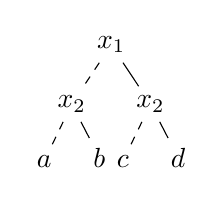
\begin{tikzpicture}[anchor=base]
    \node {$x_1$}[sibling distance = 1cm, level distance = 0.8cm]
        child  {node {$x_2$} edge from parent [dashed, sibling distance = .7cm]
            child  {node {$a$} edge from parent [dashed]}
            child {node {$b$} edge from parent [solid]};
            }
        child {node {$x_2$} edge from parent [solid, sibling distance = .7cm]
            child  {node {$c$} edge from parent [dashed]}
            child {node {$d$}}};
    \end{tikzpicture}
    \caption{The state $q$}
    \label{fig:decision_tree}
\end{subfigure}
\begin{subfigure}[b]{0.24\linewidth}
\centering
    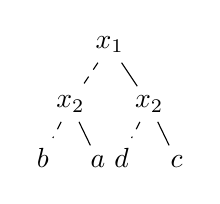
\begin{tikzpicture}[anchor=base]
    \node {$x_1$}[sibling distance = 1cm, level distance = 0.8cm]
        child  {node {$x_2$} edge from parent [dashed, sibling distance = .7cm]
            child  {node {$b$} edge from parent [dashed]}
            child {node {$a$} edge from parent [solid]};
            }
        child {node {$x_2$} edge from parent [solid, sibling distance = .7cm]
            child  {node {$d$} edge from parent [dashed]}
            child {node {$c$}}};
    \end{tikzpicture}
    \caption{Applied $\pauliX_2$}
    \label{fig:X_decision_tree}
\end{subfigure}
\begin{subfigure}[b]{0.24\linewidth}
\centering
    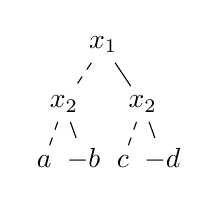
\begin{tikzpicture}[anchor=base]
    \node {$x_1$}[sibling distance = 1cm, level distance = 0.8cm]
        child  {node {$x_2$} edge from parent [dashed, sibling distance = .5cm]
            child  {node {$a$} edge from parent [dashed]}
            child {node {$-b$} edge from parent [solid]};
            }
        child {node {$x_2$} edge from parent [solid, sibling distance = .5cm]
            child  {node {$c$} edge from parent [dashed]}
            child {node {$-d$}}};
    \end{tikzpicture}
    \caption{Applied $\pauliZ_2$}
    \label{fig:Z_decision_tree}
\end{subfigure}
\begin{subfigure}[b]{0.24\linewidth}
\centering
    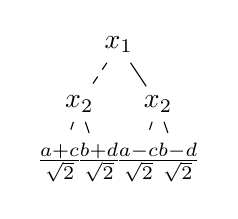
\begin{tikzpicture}[anchor=base]
    \node {$x_1$}[sibling distance = 1cm, level distance = 0.8cm]
        child  {node {$x_2$} edge from parent [dashed, sibling distance = .5cm]
            child  {node {$\frac{a+c}{\sqrt{2}}$} edge from parent [dashed]}
            child {node {$\frac{b+d}{\sqrt{2}}$} edge from parent [solid]};
            }
        child {node {$x_2$} edge from parent [solid, sibling distance = .5cm]
            child  {node {$\frac{a-c}{\sqrt{2}}$} edge from parent [dashed]}
            child {node {$\frac{b-d}{\sqrt{2}}$}}};
    \end{tikzpicture}
    \caption{Applied $\hadam_1$}
    \label{fig:H_decision_tree}
\end{subfigure}
\end{minipage}
\vspace{-3mm}
\caption{The effect of applying single-qubit quantum gates to the state $q$. }
\end{wrapfigure}
}

%%%%%%%%%%%%%%%%%%%%%%%%%%%%%%%%%%%%%%%%%%%%%%
\newcommand{\figGeneralsinglequbitgate}[0]{
\begin{wrapfigure}[7]{r}
{0.2\textwidth}%\label{fig:decision_tree}
\vspace{-4mm}
    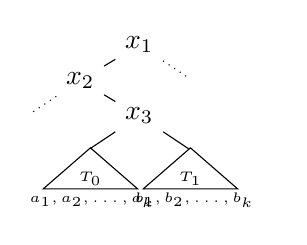
\begin{tikzpicture}[anchor=base]
    \hspace{-2mm}
    \node {$x_1$}[sibling distance = 1.5cm, level distance = 0.5cm]
        child {node {$x_2$} edge from parent [solid, sibling distance = 1.5cm]
                    child  {node {} edge from parent [dotted]}
                    child {node  {$x_3$} edge from parent [solid]
                               child {node (L) {} edge from parent [solid]}
                               child {node (R) {} edge from parent [solid]}}}
        child {node {} edge from parent [dotted, sibling distance = .7cm]};
    \draw ([xshift=0.43cm+0.3cm,yshift=-0.303cm]L.south) -- ([xshift=-0.17cm-0.3cm,yshift=-0.303cm]L.south)--([xshift=0.13cm, yshift=-0.03cm]L.north)--cycle;   
    \node at ([xshift=0.13cm, yshift=-0.203cm]L.south){\tiny $T_0$}; 
    \node at ([xshift=0.15cm,yshift=-0.48cm]L.south){\tiny $\vphantom{f}a_1,a_2,\ldots,a_k$}; 
    
    \draw ([xshift=0.43cm-0.23cm+0.3cm,yshift=-0.303cm]R.south) -- ([xshift=-0.17cm-0.23cm-0.3cm,yshift=-0.303cm]R.south)--([xshift=0.13cm-0.23cm, yshift=-0.03cm]R.north)--cycle;
    \node at ([xshift=0.13cm-0.23cm, yshift=-0.203cm]R.south){\tiny $T_1$}; 
    \node at ([xshift=0.17cm-0.22cm,yshift=-0.48cm]R.south){\tiny $\vphantom{f}b_1,b_2,\ldots,b_k$};     
    \end{tikzpicture}
    \vspace{-8mm}
    \caption{$T_0$ and $T_1$}
    \label{fig:single_gate}
\end{wrapfigure}
}

%%%%%%%%%%%%%%%%%%%%%%%%%%%%%%%%%%%%%%%%%%%%
\newcommand{\figDecisiontreecontrolled}[0]{
\begin{wrapfigure}[7]{r}{0.55\textwidth}\label{fig:decision_tree2}
  \vspace{-4mm}
\begin{minipage}{\linewidth}
\begin{subfigure}[b]{0.32\linewidth}
\centering
    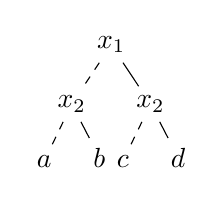
\begin{tikzpicture}[anchor=base]
    \node {$x_1$}[sibling distance = 1cm, level distance = 0.8cm]
        child  {node {$x_2$} edge from parent [dashed, sibling distance = .7cm]
            child  {node {$a$} edge from parent [dashed]}
            child {node {$b$} edge from parent [solid]}
            }
        child {node {$x_2$} edge from parent [solid, sibling distance = .7cm]
            child  {node {$c$} edge from parent [dashed]}
            child {node {$d$}}};
    \end{tikzpicture}
    \vspace{-2mm}
    \caption{The state $q$.}
    \label{fig:stateP}
\end{subfigure}
\begin{subfigure}[b]{0.32\linewidth}
\centering
    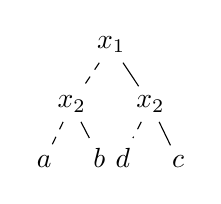
\begin{tikzpicture}[anchor=base]
    \node {$x_1$}[sibling distance = 1cm, level distance = 0.8cm]
        child  {node {$x_2$} edge from parent [dashed, sibling distance = .7cm]
            child  {node {$a$} edge from parent [dashed]}
            child {node {$b$} edge from parent [solid]};
            }
        child {node {$x_2$} edge from parent [solid, sibling distance = .7cm]
            child  {node {$d$} edge from parent [dashed]}
            child {node {$c$}}};
    \end{tikzpicture}
    \vspace{-2mm}
    \caption{Applied $\cnot^1_2$.}
    \label{fig:CX1_decision_tree}
\end{subfigure}
\begin{subfigure}[b]{0.32\linewidth}
\centering
    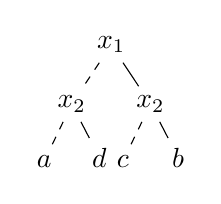
\begin{tikzpicture}[anchor=base]
    \node {$x_1$}[sibling distance = 1cm, level distance = 0.8cm]
        child  {node {$x_2$} edge from parent [dashed, sibling distance = .7cm]
            child  {node {$a$} edge from parent [dashed]}
            child {node {$d$} edge from parent [solid]};
            }
        child {node {$x_2$} edge from parent [solid, sibling distance = .7cm]
            child  {node {$c$} edge from parent [dashed]}
            child {node {$b$}}};
    \end{tikzpicture}
    \vspace{-2mm}
    \caption{Applied $\cnot^2_1$.}
    \label{fig:CX2_decision_tree}
\end{subfigure}
\end{minipage}
    \vspace{-4mm}
\caption{The effect of applying controlled gates to the state $q$.}
\end{wrapfigure}
}
%%%%%%%%%%%%%%%%%%%%%%%%%%%%%%%%%%%%%%%%%%%%%%%%%%%%%%%%%%%%%%%%%%%%%%%%%%%%%%%%
\vspace{-0.0mm}
\section{Preliminaries}
\vspace{-0.0mm}
%%%%%%%%%%%%%%%%%%%%%%%%%%%%%%%%%%%%%%%%%%%%%%%%%%%%%%%%%%%%%%%%%%%%%%%%%%%%%%%%
This section aims to provide readers with a basic understanding of quantum computing. Quantum computers are programmed through \emph{quantum gates}, and each gate
application updates the global \emph{quantum state}. A \emph{quantum circuit} is
a sequence of quantum gate applications.

%*******************************************************************************
\vspace{-0.0mm}
\subsection{Quantum States} 
\vspace{-0.0mm}
%*******************************************************************************

In a traditional computer system with~$n$ bits, a state is represented by~$n$ Boolean values. 
In the quantum world, such states are referred to as \emph{computational basis
states}.
For example, in a system with three bits labeled~$x_1$, $x_2$, and~$x_3$, the computational basis 
state $\ket{011}$ indicates that the value of~$x_1$ is~0 and the values of~$x_2$ and~$x_3$ are~1.
%\begin{changebar}
In a quantum system, an~$n$-qubit \emph{quantum state} encodes
the amplitude information of a~superposition of all possible
$n$-bit computational basis states,
%\end{changebar}
denoted as a formal sum 
$\sum_{j \in \{0,1\}^n} a_j\cdot\ket{j}$, where $a_0,a_1,\ldots,a_{2^n-1} \in
\complex$ are \emph{complex amplitudes} satisfying the property that
$\sum_{j \in \{0,1\}^n} |a_j|^2 = 1$.
% In a quantum system, an~$n$-qubit \emph{quantum state} encodes a \emph{probabilistic distribution} over $n$-bit computational basis states, denoted as a formal sum 
% $\sum_{j \in \{0,1\}^n} a_j\cdot\ket{j}$, where $a_0,a_1,\ldots,a_{2^n-1} \in
% \complex$ are \emph{complex amplitudes} satisfying the property that
% $\sum_{j \in \{0,1\}^n} |a_j|^2 = 1$.
Intuitively, $|a_j|^2$ is the probability
that when we measure the quantum state in the computational basis, we obtain the
classical state~$\ket{j}$; these probabilities must sum up to~1 for all
computational basis states. The standard representation of a quantum state is
a~vector $(a_0,a_1,\ldots, a_{2^n-1})^T$ of amplitude values, where the
superscript $T$ denotes \emph{transposition}.

We represent a~quantum state using a~\emph{decision tree} where
each branch represents a~computational basis state and the leaves hold
complex amplitudes. We demonstrate in~\cref{fig:decision_tree} an example of
a~decision tree encoding a~quantum state
$q=a\cdot\ket{00}+b\cdot\ket{01}+c\cdot\ket{10}+d\cdot\ket{11}$. This viewpoint
enables us to see the definition of standard quantum gate operations as tree
transformations.\footnote{Note that we do not discuss how to represent complex numbers; representing complex numbers precisely in computers is an
orthogonal issue to our work and can be handled by, e.g., the approach
from~\cite{ZulehnerW19} and~\cite{TsaiJJ21}.}
The viewpoint also allows us to represent a set of states compactly using \lstas.
In fact, the tree view can be generalized to handle any vector of $2^n$ entries.
We will show that \lstas can compactly represent some sets of linearly
independent vectors and use them for testing circuit equivalence.

%*******************************************************************************
\vspace{-0.0mm}
\subsection{Quantum Gates and Circuits}\label{sec:quantum_gates}
\vspace{-0.0mm}
%*******************************************************************************

The two main types of quantum gates used in state-of-the-art quantum computers are \emph{single-qubit gates} and \emph{controlled gates}. 
%We will provide an introduction of each quantum and demonstrate below how each gate operation transforms $q$, the quantum state of~\cref{fig:decision_tree}, into another decision tree.

%-------------------------------------------------------------------------------
\vspace{-0.0mm}
\subsubsection{General Single-Qubit Gates.} \label{subsubsec:general_single_qubit_gates}
\vspace{-0.0mm}
%-------------------------------------------------------------------------------
In general, a single-qubit gate is presented as a \emph{unitary complex
matrix}~$\gateof{U}$, shown below together with some common examples of this
category ($\theta$ is a parameter):
\newcommand{\spc}{\hspace{-2.5mm}}
\newcommand{\spcc}{\hspace{-2.5mm}}
%
\begin{align*}
\gateof{U}={}&
\begin{pmatrix}
 u_1 & u_2 \\
 u_3 & u_4
\end{pmatrix},&\spc
  \pauliX={}&
\begin{pmatrix}
 0 & 1 \\
 1 & 0
\end{pmatrix},&\spc
  \pauliY= {}&
\begin{pmatrix}
0 & -i\\
 i& 0
\end{pmatrix},&\spcc
  \gateRX(\theta)={}&
\begin{pmatrix}
 \cos{\frac{\theta}{2}} & -i\sin{\frac{\theta}{2}} \\
 -i\sin{\frac{\theta}{2}} & \cos{\frac{\theta}{2}}
\end{pmatrix},\ 
  \hadam=\frac 1 {\sqrt 2} 
\begin{pmatrix}
 1 & 1 \\
 1 & -1
\end{pmatrix},\\
  \pauliZ={}&
\begin{pmatrix}
1 & 0\\
 0 & -1
\end{pmatrix},&\spc
  \gateS={}&
\begin{pmatrix}
1 & 0\\
 0 & i
\end{pmatrix},&\spc
  \gateT={}&
\begin{pmatrix}
1 & 0\\
 0 & e^{\frac{i\pi}{4}}
\end{pmatrix},&\spcc
  \gateRZ(\theta) ={}&
\begin{pmatrix}
 e^{-\frac{i\theta}{2}} & 0 \\
 0 & e^{\frac{i\theta}{2}}
\end{pmatrix},\ \hspace{10mm} 
\gatePh(\theta) =
\begin{pmatrix}
 e^{i\theta} & 0 \\
 0 & e^{i\theta}
\end{pmatrix}.
\end{align*}

\figGeneralsinglequbitgate
We use $\gateof{U}_i$ to denote the application of gate $\gateof{U}$ to the
$i$-th qubit. In linear algebra, the application of a gate to a state
$(a_0,a_1,\ldots, a_{2^n-1})^T$ corresponds to the matrix multiplication
% changes \times to \cdot - \times is usually used for cross-product
$(I_{i-1}\otimes\gateof{U} \otimes I_{n-i}) \cdot (a_0,a_1,\ldots, a_{2^n-1})^T$, where $I_j$ is the $2^j$ dimensional identity matrix and $\otimes$ is the \emph{tensor product}. Under the tree view, a gate operation corresponds to a tree transformation on every two neighboring subtrees at level $i$. We use~\cref{fig:single_gate} to illustrate how the transformation $\gateof{U}_3$ works. Here $T_0$ and $T_1$ are the $0$-subtree and $1$-subtree of a node labeled $x_3$. Their leaves encode the amplitudes $a_1, a_2,\ldots, a_k$ and $b_1, b_2,\ldots, b_k$, respectively.
After applying $\gateof{U}_3$, the leaves of $T_0$ become $(u_1\cdot
a_1+u_2\cdot b_1), (u_1\cdot a_2+u_2\cdot b_2),\ldots, (u_1\cdot a_k+u_2\cdot b_k)$, obtained by multiplying the amplitudes of $T_0$ with $u_1$, those of $T_1$ with $u_2$, and summing up the two. Similarly, the leaves of $T_1$
become $(u_3\cdot a_1+u_4\cdot b_1), (u_3\cdot a_2+u_4\cdot b_2),\ldots,
(u_3\cdot a_k+u_4\cdot b_k)$. The same transformation occurs in all neighboring subtrees at the same level.
It is essential to note
that the sum of probabilities remains the same after the $\gateof{U}$ gate application,
as $\gateof{U}$ is unitary. We provide examples of applying $\pauliX_2$,
$\pauliZ_2$, $\hadam_1$ on $q$ in \cref{fig:X_decision_tree}, \cref{fig:Z_decision_tree}, and \cref{fig:H_decision_tree}, respectively.
%For instance, when applying~$\hadam_1$, there is only one pair of neighboring subtrees under the node labeled $x_1$ with leaves $(a,b)$ and $(c,d)$. Then, the new leaves will be computed as$\frac{1}{\sqrt{2}}(1 \cdot a + 1 \cdot c), \frac{1}{\sqrt{2}}(1 \cdot b + 1 \cdot d), \frac{1}{\sqrt{2}}(1 \cdot a - 1 \cdot c), \frac{1}{\sqrt{2}}(1 \cdot a - 1 \cdot d)$.


% We use $U_i$ to denote applying gate $U$ to the $i$-th qubit.  To explain how
% $U_i$ transforms $q$ (\cref{fig:decision_tree}), we first define $a_i$ and
% $b_i$ to be the $i$-th leaf value of the $0$-substrees and $1$-subtrees under
% each $x_i$, respectively.  When applying $U_1$ to $q$
% (\cref{fig:decision_tree}), for the $0$-subtree, we have $(a_1,a_2)=(a,b)$ and
% for the $1$-subsetree, we have $(b_1,b_2)= (c,d)$. When applying $U_2$, there
% are two occurrences of $x_2$ in $q$. For the left $x_2$, we have $a_1=a$,
% $b_1=b$, and the right one we have $a_1=c$, $b_1=d$. The $U_i$ gate fuses the
% $0$- and $1$-subtrees at level $i$ in such a way that the $i$-th leaf value of
% the $0$-substree becomes $(u_1*a_i+u_2*b_i)$ and the leaf value of the
% $1$-substree becomes $(u_3*a_i+u_4*b_i)$. It is essential to note that the
% probabilities' sum remains 1 after the $U$ gate application, as $U$ is
% unitary. We provide examples of applying $X_2$, $Z_2$, $H_1$ on $q$ in
% \cref{fig:X_decision_tree}, \cref{fig:Z_decision_tree}, and
% \cref{fig:H_decision_tree}, respectively.

\figDecisiontreesinglegate

%-------------------------------------------------------------------------------
\vspace{-0.0mm}
\subsubsection{Two Frequently Used Sub-categories}\label{sec:label}
\vspace{-0.0mm}
%-------------------------------------------------------------------------------

In fact, most of the quantum
gates have a simpler structure than the general case. Except the
$\gateRX(\theta)$ and $\hadam$ gates, all other considered single-qubit gates belong to the following
two categories (or their composition): (1)~the $\pauliX$ (negation) gate and
(2)~diagonal matrix ($u_2=u_3=0$) gates.
This allows more efficient automata algorithms than the general case.

The $\pauliX$ gate is the quantum ``negation'' gate. Applying $\pauliX_i$ on a
quantum state effectively swaps the $0$- and $1$-branches of all nodes at the
level $i$. An example of applying $\pauliX_2$ on $q$ is available at~\cref{fig:X_decision_tree}.

Gates with diagonal matrices, e.g., $\pauliZ$, $\gateS$, $\gateT$, $\gateRZ(\theta)$, and $\gatePh(\theta)$, multiply
all $0$- or $1$-subtrees under nodes labeled $x_i$ by the complex values
$r_0$ and $r_1$,
respectively. We note that $|r_0|$ and
$|r_1|$ always equal~$1$. We use $\gateof{D}^{r_0,r_1}$ to denote a~gate with
the diagonal matrix 
$\gateof D^{r_0,r_1} =
\big(
\begin{smallmatrix}
r_0 & 0\\
0 & r_1
\end{smallmatrix}\big)$.
We refer the reader to \cref{fig:Z_decision_tree} for an example of the
application of $\pauliZ_2=\gateof{D}_2^{1,-1}$ on $q$. 
Gates with anti-diagonal matrices, e.g., $\pauliY$, can be composed from~$\pauliX$ and $\gateof{D}^{i,-i}$ (i.e., $\pauliY = \pauliX\cdot \gateof{D}^{i,-i}$).



\subsubsection{Controlled Gates.}

A~controlled gate $\gateof{CU}$ uses another quantum gate $\gateof{U}$ as its
parameter. $\gateof{CU}$~has
a~control qubit~$x_c$ and the gate $\gateof U$ is applied only when the control
qubit~$x_c$ has value~$1$.
The controlled $\pauliX$ gate $\cnot^1_2$ has the control qubit
$x_1$ and would apply $\pauliX_2$ when $x_1$ is valued $1$.\figDecisiontreecontrolled   %%%%%%%%%%%%
The result of applying $\cnot^1_2$ on $q$ is available in~\cref{fig:CX1_decision_tree}.
Observe that $\pauliX_2$ is only applied to the $1$-subtree of $x_1$. 
On the other hand, the result of applying $\cnot^2_1$ on $q$ is available in
\cref{fig:CX2_decision_tree}. Observe that all $0$-subtrees at level $2$ remain
the same as in~$q$, but the $1$-subtrees at level $2$ are updated to the
corresponding ones after applying the $\pauliX_1$ gate to $q$.


\subsubsection{Quantum Circuits.} As we mentioned before, a quantum circuit is a
sequence of quantum gates. Executing a~circuit effectively performs a sequence of tree updates
following the gates' semantics. We often represent a quantum circuit using a
diagram as in~\cref{fig:ERPcircuit}, which is also written as $H_1 CX^1_2$.
% \ol{changed because of the change in the figure}

%\begin{changebar}
As an analogy, in classical circuits, a~state corresponds to a~computational
basis state, and a~gate application transforms one basis state to another.
This process can be represented using a~single tree branch.
In contrast, encoding quantum states requires accounting for the amplitude values of all computational basis states, which necessitates using a complete tree structure for representation.
Our method captures key quantum-specific features, particularly the ability to
encode superpositions of basis states and their associated amplitudes.
While our methods can be adapted to verify classical circuits by simplifying
the state representation and adding support to classical gates, the primary
distinction lies in our approach to handling quantum superposition and gate
semantics---features that are absent in classical computation.
%\end{changebar}


%%%%%%%%%%%%%%%%%%%%%%%%%%%%%%%%%%%%%%%%%%%%%%%%%%%%%%%%%%%%%%%%%%%%%%%%%%%%%%%%
\vspace{-0.0mm}
\section{Level-Synchronized Tree Automata}\label{sec:cta}
\vspace{-0.0mm}
%%%%%%%%%%%%%%%%%%%%%%%%%%%%%%%%%%%%%%%%%%%%%%%%%%%%%%%%%%%%%%%%%%%%%%%%%%%%%%%%

In this paper, a new tree automata model called \emph{Level-Synchronized Tree Automata} (\lstas) is developed.
The expressiveness of this model is incomparable with the traditional tree automata model (\cref{thm:expressiveness}) while
maintaining important properties such as being closed under union and intersection. It also allows for testing language emptiness and inclusion, enabling the testing of whether all reachable states are included in the post-condition.
One crucial advantage of \lstas is that they annotate transitions with ``choices'' and use them to
coordinate between tree branches, enabling efficient quantum state encoding and gate operations (see~\cref{sec:quantum_gates}).

%*******************************************************************************
\vspace{-0.0mm}
\subsection{Formal Definition of \lstas}
\label{sec:lstabasics}
\vspace{-0.0mm}
%*******************************************************************************

\paragraph{Binary Trees.} 
We use $\nat$ to represent the set of natural numbers
(without~0), $\natz=\nat\cup\{0\}$ to represent the set of non-negative integers, and $\bool = \{0,1\}$ to represent the Boolean values.
A~ranked alphabet is a set of symbols $\Sigma$ with a corresponding rank given by a~function $\arity\colon\Sigma\to\{0,2\}$. The symbols with rank $0$ are called 
%\emph{constant} or 
%\lu{\emph{constant} is never used, only one occurrence few lines below, that can be replace by leaf symbol. I am removing it, ok?}
\emph{leaf} symbols, and those with rank $2$ are called \emph{internal} symbols.

%In mathematical notation, we use $\nat$ to represent the set of natural numbers
%(without~0), $\natz$ to represent the set of non-negative integers
%$\natz=\nat\cup\{0\}$, and $\bool = \{0,1\}$ to represent the Boolean values.
%A~ranked alphabet is a set of symbols $\Sigma$ with a corresponding rank given by a~function $\arity\colon\Sigma\to\{0,2\}$. The symbols with rank $0$ are called \emph{constant} or \emph{leaf} symbols, and those with rank $2$ are called \emph{internal} symbols.


A~\emph{binary tree} is a finite map $T\colon \{0,1\}^*\rightarrow \Sigma$ that maps \emph{tree nodes} (i.e., words over the alphabet~$\{0,1\}$) to symbols in $\Sigma$, and satisfies that
%
\begin{inparaenum}
    \item the domain of $T$ is \emph{prefix-closed} and
    \item if $T(v) = f$ and $f$ is internal, then the set of \emph{children} of $v$ in $T$ is $\{v.0,v.1\}$, and if $f$ is a leaf symbol then $v$ has no children.
\end{inparaenum}
Nodes labeled by leaf symbols and internal symbols are called \emph{leaf nodes} and \emph{internal nodes}, respectively. 
A node's \emph{height} is its word length, denoted~$\height(w)$; e.g., $\height(01010) = 5$.
A node $w$ is at tree level $i$ when $\height(w)=i$. A tree is \emph{perfect} if all leaf nodes have the same height. We need only \emph{perfect binary trees} to represent quantum states or vectors of sizes $2^n$.
\begin{example}
The quantum state of~\cref{fig:state} corresponds to a tree $T$ with
  $T(\epsilon)=x_1$, $T(0)=T(1)=x_2$, $T(00)=T(11)=0$, and
  $T(01)=T(10)=\frac{1}{\sqrt{2}}$, where $\epsilon$ is an empty string. We have
  $\dom(T)=\{\epsilon, 0,1,00,01,10,11\}$. Children of the node $0$ are $00$ and $01$.
  The leaf node $01$ has no children.
\end{example}

%We sometimes write trees as terms, e.g., the tree in \cref{fig:decision_tree} can be written as the term $x_1(x_2(a,b), x_2(c,d))$.

\begin{definition}
A~\emph{level-synchronized tree automaton} (\lsta) is a~tuple $\aut = \tuple{Q, \Sigma, \Delta, \rootstates}$ where 
\begin{enumerate}
    \item $Q$ is a~finite set of \emph{states}, $\rootstates \subseteq Q$ is a~set of \emph{root states}, and $\Sigma$~is a~ranked alphabet.
    \item $\Delta$ is a set of  transitions of the form
      $\ctranstreenoset q f {q_1,q_2}{C}$ (\emph{internal trans.}) or $\ctranstreenoset q f {}{C}$ (\emph{leaf trans.}), where
      $C\subseteq \natz$ is a~finite set of \emph{choices} (represented as natural
      numbers), $q, q_1, q_2 \in Q$, and $f\in \Sigma$. In figures, we draw internal and leaf transitions as $\tikztrans{q}{C}{f}{q_1}{q_2}$ and $\tikzleaftrans{q}{C}{f}$.
      
    \item We call $q$, $f$, $C$, and $\{q_1,q_2\}$ the \emph{top}, the \emph{symbol}, the \emph{choices}, and the \emph{bottom}, respectively, of the transition $\delta$, 
and denote them by $\topof \delta$, $\symof \delta$, $\ell(\delta)$, and $\botof \delta$, respectively. We use $|\aut|$ to denote $\aut$'s number of states.
    \item We further require that the choices of transitions with the same top
      state are disjoint, i.e., $\forall \delta_1\ne\delta_2\in\Delta\colon \topof{\delta_1}=\topof{\delta_2}\implies\ell(\delta_1)\cap\ell(\delta_2)=\emptyset$
\end{enumerate}    
\end{definition}
%Let us provide a few examples of \lsta-based encoding of sets of quantum states. We first formalize Examples \thecexBell\ and \thecexGHZ\ from Introduction. %\cref{sec:intro}.

%\figNGHZpost   %%%%%%%%%%%%%%%%%%%%%%%



%\figGHZState
%The concept of \emph{level-synchronization} is the key to the exponential space saving. Notice that each of the GHZ states has ``mirrored'' $0$- and $1$-
%subtrees (\cref{fig:ghz-state-tikz}); if the $0$-subtree is $\frac{1}{\sqrt{2}}\ket{b_2b_3\ldots b_n}$, then the $1$-subtree
%is either $\frac{ 1}{\sqrt{2}}\ket{\bar{b_2}\bar{b_3}\ldots \bar{b_n}}$ or $\frac{-1}{\sqrt{2}}\ket{\bar{b_2}\bar{b_3}\ldots \bar{b_n}}$. At each level of~\cref{fig:bell_states}, the labeled choices can be used to match a $b_i$ transition of the $0$-subtree with a $\bar{b}_i$ transition of the $1$-subtree, for $b_i\in \{0,1\}$. Together with the transition connecting to zero amplitude values, $\lsta$ needs only $5$ more transitions for one more qubit.


\paragraph{The Language of an~\lsta}
A \emph{run} of an \lsta $\aut$ on a~tree $T$ is a total map $\run\colon \dom(T) \rightarrow \Delta$ from tree nodes to transitions of~$\aut$ such that for each node $v\in \dom(T)$, 
%$\run(v)$ is of the form $\tikztrans{q}{}{T(v)}{\topof{\run(v.0)}}{\topof{\run(v.1)}}$ when $v$ is internal and $\tikzleaftrans{q}{}{T(v)}$ when $v$ a leaf node.
when $v$ is an internal node, $\run(v)$ is of the form $\ctranstreenoset {q} {T(v)} {q_0,q_1} C$, where the two bottom states $q_0=\topof{\run(v.0)}$ and $q_1=\topof{\run(v.1)}$ are the two top states of $v$'s children $\run(v.0)$ and $\run(v.1)$. When $v$ is a~leaf node, $\run(v)$ is of the form $\ctranstreenoset {q} {T(v)} {} C$.

\begin{example}\label{ex:lstarun}
We define a \emph{run} $\rho$ of the \lsta $\aut$ in~\cref{fig:bell_states} on the tree $T$ in~\cref{fig:state} as follows. We have 
%$\rho(\epsilon)=\ctikztrans {p} {1} {x_1} {q_{+}} {q_{\pm}}$, 
%$\rho(0)=\ctikztrans {q_{+}} {2} {x_2} {r_{0}} {r_{+}}$, 
%$\rho(1)=\ctikztrans {q_{\pm}} {2} {x_2} {r_{\pm}} {r_{0}}$, 
%$\rho(01)=\ctikzleaftrans {r_{+}} {1,2} {\frac{1}{\sqrt{2}}}$, 
%$\rho(00)=\rho(11)=\ctikzleaftrans {r_0} {1,2} {0} $, and 
%$\rho(10)=\ctikzleaftrans {r_{\pm}} {1} {\frac{1}{\sqrt{2}}}$.
%
%  $\rho(\epsilon)= \ctranstree {p} {x_1} {q_{+}, q_{\pm}}{1}$, 
%  $\rho(0)=\ctranstree {q_{+}} {x_2} {r_{0}, r_{+}}{2}$, 
%  $\rho(1)=\ctranstree {q_{\pm}} {x_2} {r_{\pm}, r_{0}}{2}$, 
%  $\rho(01)=\ctranstree {r_{+}} {\frac{1}{\sqrt{2}}} {}{1,2}$, 
%  $\rho(00)=\rho(11)=\ctranstree {r_0} {0} {}{1,2}$, and 
%  $\rho(10)=\ctranstree {r_{\pm}} {\frac{1}{\sqrt{2}}} {}{1}$.
%
\begin{flalign*}
  &&
  \rho(\epsilon)&{}= \ctranstree {p} {x_1} {q_{+}, q_{\pm}}{1}, 
  &
  \rho(0)&{} =\ctranstree {q_{+}} {x_2} {r_{0}, r_{+}}{2}, 
  &
  \rho(1)&{}=\ctranstree {q_{\pm}} {x_2} {r_{\pm}, r_{0}}{2}, \\ 
  &&  
  \rho(01)&{}=\ctranstree {r_{+}} {\tfrac{1}{\sqrt{2}}} {}{1,2},
  &
  \rho(10)&{}=\ctranstree {r_{\pm}} {\tfrac{1}{\sqrt{2}}} {}{1},
  &
  \rho(00)=\rho(11)&{}=\ctranstree {r_0} {0} {}{1,2}.& 
 \hspace{-14mm}\qed
\end{flalign*}

%\begin{flalign*}
%  &&
%  \rho(\epsilon)&{}= \ctranstree {p} {x_1} {q_{+}, q_{\pm}}{1}, 
%  &
%  \rho(01)&{}=\ctranstree {r_{+}} {\frac{1}{\sqrt{2}}} {}{1,2},
%  \\ &&
%  \rho(0)&{} =\ctranstree {q_{+}} {x_2} {r_{0}, r_{+}}{2}, 
%  &
%  \rho(10)&{}=\ctranstree {r_{\pm}} {\frac{1}{\sqrt{2}}} {}{1},
%  \text{ and}
%  \\ &&
%  \rho(1)&{}=\ctranstree {q_{\pm}} {x_2} {r_{\pm}, r_{0}}{2}, 
%  &
%  \rho(00)=\rho(11)&{}=\ctranstree {r_0} {0} {}{1,2}.
%  &
% \qed
%\end{flalign*}
\end{example}

We define the \emph{level} $d$ of a run $\run$ as the set of transitions with height $d$
$$ \level(\run,d):= \{\run(w) \mid  w \in \dom(T) \land \height(w)=d\}\ .$$

The run $\rho$ is \emph{accepting} if $\topof{\rho(\epsilon)}\in\rootstates$ and
all transitions from the same level share some common choice, i.e., $\forall
d\in \nat\colon\bigcap_{\delta\in\level(\run,d)}\ell(\delta)\neq\emptyset$---in other words, transitions at each tree level are \emph{synchronized}.
The \emph{language} of $\aut$ is the set $\langof \aut$ of trees~$T$ with an accepting run.

\begin{example}
%Continue from~\cref{ex:lstarun}. We have $\level(\run,1):= \{\ctikztrans {q_{+}}{2}{x_2}{r_{0}}{r_{+}}, \ctikztrans {q_{\pm}}2{x_2} {r_{\pm}}{r_{0}}\}$ and $\level(\run,2)=\{\ctikzleaftrans {r_{+}}{1,2}{\frac{1}{\sqrt{2}}}, \ctikzleaftrans {r_0}{1,2}{0}, \ctikzleaftrans {r_{\pm}}{1}{\frac{1}{\sqrt{2}}}\}$. Observe the $\rho$ is accepting because $\topof{\rho(\epsilon)}=p \in \rootstates$, the transitions from $\level(\run,1)$ have a common choice $2$, and those from $\level(\run,2)$ have a common choice $1$.
 Continuing from~\cref{ex:lstarun}, we have $\level(\run,1) = \{\ctranstree
  {q_{+}} {x_2} {r_{0}, r_{+}}{2}, \ctranstree {q_{\pm}} {x_2} {r_{\pm},
  r_{0}}{2}\}$ and $\level(\run,2)=\{\ctranstree {r_{+}} {\frac{1}{\sqrt{2}}}
  {}{1,2}, \ctranstree {r_0} {0} {}{1,2}, \ctranstree {r_{\pm}}
  {\frac{1}{\sqrt{2}}} {}{1}\}$. Observe that~$\rho$ is accepting because $\topof{\rho(\epsilon)}=p \in \rootstates$, the transitions from $\level(\run,1)$ have a common choice $2$, and those from $\level(\run,2)$ have a common choice~$1$.
  \qed
\end{example}

%We defer the details of the properties of \lstas to~\cref{sec:lsta_alg} to make
%the flow of reading smoother. 
We defer a detailed discussion on properties of \lstas to~\cref{sec:lsta_alg}. 
At this point, we just note that the
\emph{inclusion test} over \lstas, i.e., checking if $\langof{\aut_1}\subseteq
\langof{\aut_2}$ for \lstas $\aut_1$ and $\aut_2$, is decidable.


%%%%%%%%%%%%%%%%%%%%%%%%%%%%%%%%%%%%%%%%%%%%%%%%%%
\newcommand{\figBVcircuit}[0]{
\begin{wrapfigure}[14]{r}{0.42\textwidth}
    \vspace{-5mm}
    \centering
    \scalebox{0.7}{
    \begin{quantikz}
    \lstick{$\ket{s_1}$}\gategroup[wires=1,steps=8,style={rounded corners,fill=blue!10,draw opacity=0},background]{} && \ctrl{7} \gategroup[wires=8,steps=4,style={dashed,
    rounded corners,fill=blue!10,draw opacity=0},background]{} &&&&& \\
    \lstick{$\ket{0}$} & \gate{H} & \ctrl{0} &&&& \gate{H} & \\
    \lstick{$\ket{s_2}$}\gategroup[wires=1,steps=8,style={rounded corners,fill=blue!10,draw opacity=0},background]{} &&& \ctrl{5} &&&&\\
    \lstick{$\ket{0}$} & \gate{H} && \ctrl{0} &&& \gate{H}  & \\
    \lstick{$\dots$}  \\
    \lstick{$\ket{s_n}$}\gategroup[wires=1,steps=8,style={rounded corners,fill=blue!10,draw opacity=0},background]{} &&&&& \ctrl{2} &&\\
    \lstick{$\ket{0}$} & \gate{H} &&&& \ctrl{0} &\gate{H}  &\\
    \lstick{$\ket{1}$} & \gate{H} & \targ{} & \targ{} & \dots & \targ{} & \gate{H} &
    \end{quantikz}
    }

    \vspace{-2mm}
    \caption{BV circuit. Standard Toffoli gates have two $\bullet$ as controls
    and one $\oplus$ as the target.}
    \label{fig:bv-circuit}
\end{wrapfigure}
}

%%%%%%%%%%%%%%%%%%%%%%%%%%%%%%%%%%%%%%%%%%%%%%%%%%%%%%%%%%%%%%%%%%%%%%%%%%%%%%%%
\vspace{-0.0mm}
\section{Using \lstas to Describe Correctness Properties}
\label{sec:properties}
\vspace{-0.0mm}
%%%%%%%%%%%%%%%%%%%%%%%%%%%%%%%%%%%%%%%%%%%%%%%%%%%%%%%%%%%%%%%%%%%%%%%%%%%%%%%%
We can use an \lsta to encode a set of perfect binary trees (quantum states or
vectors) and use them as pre- and post-conditions for verification of quantum
circuits.
Below, we will provide examples of the verification problems and the
corresponding specifications given using \lstas.

%*******************************************************************************
\vspace{-0.0mm}
\subsection{Verification of Oracle-Based Algorithms}\label{sec:oracle}
\vspace{-0.0mm}
%*******************************************************************************

\figBVcircuit  %%%%%%%

% \paragraph{The verification of oracle-based algorithms:}
An \emph{oracle circuit} is a black box circuit used to encode a~specific
function. It plays a crucial role in many quantum algorithms by providing a way
to query information in a single computational step. In the case of Grover's
search algorithm~\cite{Grover96}, the oracle circuit encodes a function
$f(x)\colon \bool^n \to \bool$ that outputs $1$ if $x$ is the solution
and~$0$ otherwise. In the case of the Bernstein-Vazirani
algorithm~\cite{BernsteinV93}, the oracle circuit encodes a~secret bit string.
To verify the correctness of these algorithms against all possible oracles, one
way is to create a \emph{parameterized} oracle circuit that uses input qubits
and control gates to generate the corresponding oracle.
By composing the parameterized oracle circuit and the circuit to be verified, we
can create a framework to verify the correctness of these circuits against
all oracles.

Taking verification of the Bernstein-Vazirani algorithm (BV) as an example, the
composed circuit consists of $2n+1$ qubits (\cref{fig:bv-circuit}), where the
highlighted part $\bluelab{\ \ }$ is the oracle circuit and the rest is the circuit under verification.
%\begin{changebar}
We emphasize that in our setting, we consider parameterized oracle with the
secret provided as a~part of the input of the circuit.
%\end{changebar}
The qubits $s_1,s_2,\ldots, s_n$ serve as the input for the parameterized oracle circuit, and the other qubits act as the working tape of the circuit being verified, particularly, the last qubit acts as the ancilla, i.e., an \emph{auxiliary variable} in the sense of classical program verification.
We will verify the correctness of the implementation using the precondition
$\{\ket{s_10s_20\ldots s_n01}\mid s_1,s_2,\ldots s_n\in \bool\}$ and the
postcondition $\{\ket{s_1s_1s_2s_2\ldots s_ns_n1}\mid s_1,s_2,\ldots s_n\in
\bool\}$.
That is, considering all possible secret strings $s_1s_2\ldots s_n$ as the input
of the oracle circuit and verifying that the BV circuit finds the same string at the output.
We show the \lsta representing the postcondition in~\cref{fig:bv-post}.
In this \lsta, the states $q_0^i$ generate subtrees with leaves~$0$. 
From the state $q^i$, the \lsta picks a secret bit $b$ using the disjunctive branch, remembers it in states $q_R^{i+1}$ ($b=1$) or $q_L^{i+1}$ ($b=0$), and repeats the value in the next transition.
The precondition can be modeled in a similar manner to~\cref{fig:bv-post} and,
hence, omitted. 

\figBVpost  %%%%%%%%

%%%%%%%%%%%%%%%%%%%%%%%%%%%%%%%%%%%%%%%%%%%%%%%%%%%%%%


%*******************************************************************************
\vspace{-0.0mm}
\subsection{Verification of Compound Multi-Control Quantum Gates}\label{sec:multi-control}
\vspace{-0.0mm}
%*******************************************************************************

\figMCToffoli  %%%%%%%%%%

% \emph{The verification of compound quantum gate:}
When implementing quantum algorithms on quantum computers, which have a~limited
set of supported gates, one often needs to find a~way how to implement an
unsupported gate by composing several natively supported gates.
% When working with quantum computers, it is common to encounter quantum gates
% that are not natively supported.
% In such cases, we can achieve the desired functionality by combining several supported gates.
For instance, the multi-control Toffoli gate is not typically supported and
is often created using standard Toffoli gates (cf.~\cref{fig:cccx}).
In this type of circuit, qubits $\ket{c_1},\ldots,\ket{c_n}$ serve as the
control, those $\ket{0}$ below the controlled qubits are the ancilla qubits, and
the last qubit~$\ket t$ is the target. For this circuit to be correct, it should hold
that
(1)~it maps ancilla qubits $\ket{0^{n-1}}$ to $\ket{0^{n-1}}$ (we do not impose any
restrictions on the behavior of the circuit if the input ancillas are not
$\ket{0^n}$) and
(2)~the operation of the circuit on the rest of the qubits is equivalent to a
multi-control Toffoli gate, i.e.,
% it maps $\ket{s_1,\ldots, s_n, s_{n+1}}$ to $\ket{s_1,\ldots, s_n,
% (s_1\land\ldots\land s_n) \oplus s_{n+1}}$ for all $ s_1,\ldots, s_n, s_{n+1}\in
% \{0,1\}$.
for computational bases of the form $\ket{c_1\ldots c_n t}$, it swaps the amplitudes of
bases $\ket{1^n 0}$ and $\ket{1^n1}$ and keeps all the other
bases the same.
%\ol{please YFC check that it is correct}\yfc{ok}
% it maps the amplitude$\ket{c_1\ldots c_n t}$ to $\ket{c_1\ldots c_n
% ((c_1\land\ldots\land c_n) \oplus t)}$ for all $c_1,\ldots, c_n, t\in
% \bool$ where $\oplus$ denotes \ol{what? and what does $\land$ denote when we
% talk about qubits?}.

%\ol{the CCNOTs in the figure were not introduced (the notation, i.e., how we draw them). This is already the case for Fig. 1}\yfc{addressed}


A~fundamental issue with specifying the functionality of such circuits using
Hoare triples is that we need to express a~mapping between input and output quantum
states, which is not directly expressible
using only sets of states\footnote{One could, indeed, make a~copy of the input
qubit values, but this would cause a~blow-up in the size of the underlying
representation, losing the compactness of \lstas.}.
In the case of multi-control gates, we can use the fact that the values of the control qubits should
not change at the output, and we only care about the case the values of the ancillas remain $0$, the only qubit whose value will change is the target~$\ket t$.
Hence, we reduce the verification problem to two sub-problems against the two
pairs of pre- and postconditions $\mbox{Pre}_k$ and $\mbox{Post}_k$ below, for
the value of~$\ket t$ being $k\in\bool$.
%
% \begin{align*}
%     \mbox{Pre$_k$}={}&\{\ket{\overset{\text{\vphantom{g}ancillas}}{\overbrace{0^{n-1}}}\overset{\text{\vphantom{g}controls}}{\overbrace{\vphantom{0^{n-1}}c_1\ldots
%     c_n}} \overset{\text{target}}{\overbrace{\vphantom{0^{n-1}}k}}}\mid c_1,\ldots, c_n\in \bool\} &&&
%     \mbox{Post$_k$}={}&(\mbox{Pre$_k$} \setminus \{\ket{0^{n-1}1^n k}\}) \cup
%     \{\ket{0^{n-1}1^n\bar{k}}\}
%     % \mbox{Post$_k$}={}&\{\ket{c_1 c_2 0 c_3 0 \ldots c_n 0 ((c_1\land\ldots\land
%     % c_n) \oplus k)}\mid c_1,\ldots, c_n\in \bool\}
% \end{align*}
% \yfc{the qubit order is wrong}
%
% \begin{align*}
%     \mbox{Pre$_k$}={}&\{\ket{c_1 c_2 0 c_3 0 \ldots c_n 0 k}\mid c_1,\ldots,
%     c_n\in \bool\}&
%     \mbox{Post$_k$}={}&(\mbox{Pre$_k$} \setminus \{\ket{11010\ldots10k}\}) \cup
%     \{\ket{11010\ldots10\bar{k}}\}
%     % \mbox{Post$_k$}={}&\{\ket{c_1 c_2 0 c_3 0 \ldots c_n 0 ((c_1\land\ldots\land
%     % c_n) \oplus k)}\mid c_1,\ldots, c_n\in \bool\}
% \end{align*}
%
\begin{align*}
    % \mbox{Pre$_i$: }&\{\ket{s_1,s_2,0,s_3,0,\ldots, s_n,0,i}\mid s_1,\ldots, s_n\in \{0,1\}\}\\ 
    % \mbox{Post$_i$: }&\{\ket{s_1,s_2,0,s_3,0,\ldots, s_n,0,(s_1\land\ldots\land s_n) \oplus i}\mid s_1,\ldots, s_n\in \{0,1\}\}
    \mbox{Pre$_k$}={}&\{\ket{c_1 c_2 0 c_3 0 \ldots c_n 0 k}\mid c_1,\ldots, c_n\in \bool\}\\
    \mbox{Post$_k$}={}&\{\ket{c_1 c_2 0 c_3 0 \ldots c_n 0 k'}\mid c_1,\ldots, c_n\in \bool, k'= (c_1\land\ldots\land
    c_n) \oplus k\}
\end{align*}
%
Intuitively, the postcondition says that if all control qubits are set to~1,
then the value of the target should be flipped (denoted using the xor
operator~$\oplus$).
\mbox{Pre$_k$} and \mbox{Post$_k$} can be modelled using \lstas in
a~similar way as in \cref{fig:bv-post}.
Specification of other multi-control gates could be done likewise.
%
% One difficulty we encountered was that our specification was given in the form
% of two sets, but here, we needed to model the functionality of a map between
% quantum states. The trick we used here is based on the observation that the
% control qubits are only affected by control gates, therefore their values
% remain the same after the circuit execution. We will use this observation to
% identify the correspondence between the input and the resulting state in the
% pre- and post-conditions.
% Hence, we reduce the verification problem to two sub-problems against the two
% pairs of pre- and postconditions $\mbox{Pre}_k$ and $\mbox{Post}_k$ below, for
% $k\in\bool$.
% One handles the case when the target qubit value is initially $0$ and the other for the $1$ case. The same approach can be used to verify the implementation of other multi-control gates. 

\newcommand{\figEqVec}[0]{
% eq vectors
\begin{wrapfigure}[9]{r}{0.65\textwidth}
    \centering
    \vspace{-4mm}
    \scalebox{0.7}{
      \input{figs/eq-check.tikz}
    }
    \vspace{-7mm}
    \caption{LSTA for the pre- and post-condition for equivalence
    checking}
    \label{fig:EqBasis}
\end{wrapfigure}}



%*******************************************************************************
\vspace{-0.0mm}
\subsection{Equivalence Checking}\label{sec:equivalence_checking}
\vspace{-0.0mm}
%*******************************************************************************

\figEqVec
% \emph{Equivalence checking:}
When considering the \lsta model's expressiveness as a~specification language, it
is interesting to note that it can be used to express that a circuit implements
the \emph{identity} function, allowing for checking of circuit equivalence.
More precisely, given two circuits $C_1$ and $C_2$, we can check if they are
%\begin{changebar}
equivalent by checking if $C_1C_2^\dag$ is an identity, where $C_2^\dag$ can be
obtained from~$C_2$ by reverting it (i.e., inputs are swapped with outputs) and
substituting every gate by its inverse.
%\ol{is it correct?}
Since all quantum gates correspond to unitary matrices, their inverses can be
obtained by taking their conjugate transpose.
For instance,
the inverse of a single qubit gate $U=\big(
\begin{smallmatrix}
u_1 & u_2\\
u_3 & u_4
\end{smallmatrix}\big)$ is the gate $U^\dag = \big(
\begin{smallmatrix}
\overline{u_1} & \overline{u_3} \\
\overline{u_2} & \overline{u_4}
\end{smallmatrix}\big)$
in the same form, where $\overline{u}$ is the complex conjugate of $u$
(therefore, whenever we can implement the gate~$U$, we can also obtain an
implementation of the gate~$U^\dag$).
%\end{changebar}
    %%%%%%%%

We can then verify if an $n$-qubit circuit is an identity by testing it against
$2^n$ linearly independent \emph{vectors} and checking if each resulting vector
matches its input vector (this is due to the fact that the identity matrix is the
only matrix that maps all vectors back to themselves; due to linearity, it
suffices to only try a~maximal set of linearly independent vectors).
Using \lstas, all $2^n$ of these tests can be performed simultaneously. 
%\begin{changebar}
We use trees corresponding to the set of vectors $\{(0,0,\ldots,1),\ldots,(0,1,\ldots,1), (1,1,\ldots,1)\}$\footnote{The set can be defined formally as the set $\{(b_1, b_2, \ldots, b_{2^n}) \in \{0,1\}^{2^n} \mid 0\leq b_1 \leq b_2 \leq \ldots \leq b_{2^n} = 1\}$.} simultaneously as both the precondition and the postcondition.
%\end{changebar}
The corresponding \lsta can be found in~\cref{fig:EqBasis}, with the number of transitions linear to the number of qubits. We note three key observations: 
\begin{inparaenum}[(i)]
\item the set of vectors is linearly independent, 
\item the vectors do not represent quantum states, which is fine due to the linearity of quantum gate operations, and
\item each vector has a unique number of ones; therefore, every vector has a distinct \emph{Euclidean norm}. Since quantum gates are unitary operators, this norm is preserved, ensuring that there will be exactly one vector with the specified norm in the output. 
\end{inparaenum}
Note that not all linearly independent set of vectors can be used, such as the
standard basis of $\reals^{2^n}$, since the vectors there have the same norm, so
we would lose the one-to-one correspondence between the input and output vectors.
% \ol{I'm making things up :-). Can someone with any knowledge of linear algebra
% check what I wrote? :-D} \yfc{some orthonormal basis }

% It is important to note that this set of vectors is linearly independent.
% The number of nonzero leaf values is different in each vector and, therefore,
% can be used to maintain the correspondence between the input and resulting
% vectors.

% It is important to note that this set of vectors is linearly independent.
% The number of nonzero leaf values is different in each vector and, therefore,
% can be used to maintain the correspondence between the input and resulting
% vectors.

% \ol{should we emphasize that the vectors do not correspond to quantum states?}
%
% \ol{maybe mention why using one-hot vectors (which could be encoded compactly
% using TAs) wouldn't work}


%*******************************************************************************
\vspace{-0.0mm}
\subsection{Verification of Amplitude Constraints}\label{sec:amplitude}
\vspace{-0.0mm}
%*******************************************************************************
\figAmplitude


% \emph{The verification of amplitude constraints:}
Similarly to the work of~\cite{ChenCLLT23}, \lstas can be extended to
support symbolic amplitudes.
For example, when verifying an amplitude amplification algorithm (such as
Grover's search~\cite{Grover96}), we can use variables~$v_h$ and~$v_l$ as
amplitudes (leaf labels) of the \lsta representing the
precondition and describe the relation between the two variables using a~global
constraint, such as
$\varphi\colon|v_h+3v_\ell|>|2v_h|$, which was used in~\cite{ChenCLLT23} for
Grover's search.
A~tree accepted by such an \lsta is in~\cref{fig:tree_aa}
and the output obtained after symbolically executing a~circuit~$C$
that amplifies the amplitude of~$\ket{00}$ over the tree is in
\cref{fig:tree2_aa}.
At the post-condition \lsta, we label the leaves with predicates in the form of
$|\square|^2 > |x|^2$ or $|\square|^2 > 90\%$ to denote that the matching leaf
probability (denoted as $|\square|^2$) should be bigger than the value of the
precondition~$|x|^2$ or the constant~90\,\%, respectively, for~$x$ being some of
the used variables.
In~\cref{fig:tree3_aa}, we demonstrate an example of a tree accepted by the
post-condition \lsta.
Notice that if we put all leaf amplitudes of~\cref{fig:tree2_aa} into the
matching $\square$ of the tree in~\cref{fig:tree3_aa}, the resulting formula is
implied by the global constraint $\varphi$.
For example, for the branch $\ket{00}$, we have that $|v_h+3v_\ell|>|2v_h|
\implies |\frac{v_h+3v_l}{2}|^2 > |v_h|^2$ is valid.
In such a case, we say that the resulting tree is accepted in the post-condition.
The symbolic extension would allow us to verify a circuit against properties
such as that the full Grover's circuit has ${>}90\,\%$ probability of finding a
correct answer or that an \emph{amplitude amplification} algorithm increases the
probability of finding a correct answer in each iteration. 

%%%%%%%%%%%%%%%%%%%%%%%%%%%%%%%%%%%%%%%%%%%%%%%%%%%%%%
\newcommand{\figSingleQubitExample}[0]{
\begin{figure}
     \begin{subfigure}[b]{0.2\textwidth}
     \scalebox{0.65}{
       \input{figs/epr-pre.tikz}
     }
    \caption{Basis states}\label{fig:basis_state}
     \end{subfigure}
    \begin{subfigure}[b]{0.5\textwidth}
    \centering
    \scalebox{0.65}{
      \input{figs/single-qubit-h1.tikz}
        }
    \caption{Applying $\hadam_1$ to the LSTA from~(\subref{fig:basis_state})}
    \label{fig:eprafterH}
    \end{subfigure}
    \begin{subfigure}[b]{0.28\textwidth}
    \centering
    \scalebox{0.65}{
      \input{figs/single-qubit-min.tikz}
    }
    \caption{Reduced \lsta from (\subref{fig:eprafterH})}
    \label{fig:eprafterHmin}
    \end{subfigure}

\vspace{-2mm}
\caption{An example of applying a single-qubit gate on a~set of quantum states
  represented using an \lsta.}
% \vspace{-6mm}
\label{fig:single_qubit_example}
\end{figure}
}

%%%%%%%%%%%%%%%%%%%%%%%%%%%%%%%%%%%%%%%%%%%%%%%%%%%%%%%%%%%%
\newcommand{\algUGate}[0]{
\begin{figure}[t]
\resizebox{\textwidth}{!}{
\begin{minipage}{1.20\linewidth}
\begin{algorithm}[H]
\caption{Application of a~single-qubit gate on an \lsta}
\label{algo:u_gate_single}
\KwIn{An \lsta $\aut=\tuple{Q, \Sigma, \Delta, \rootstates}$ and a gate $\gateof{U}_t=\big(\begin{smallmatrix}
         u_{1} & u_{2} \\
        u_{3} & u_{4}
        \end{smallmatrix}\big)$}
\KwOut{$\gateof{U}_t(\aut)$}
$\ctr{\Delta'_{< t}}{\ell'_{< t}} := \{ {\ctranstreenoset {q} {x_i}
{q_l,q_r}{C}} \in \Delta \mid i<t\}$\;
$\ctr{\Delta'_{= t}}{\ell'_{= t}} := \{ \ctranstreenoset q {x_t}
{(q_l,q_r,L),(q_l,q_r,R)}{C} \mid 
\ctranstreenoset q {x_t}
{q_l,q_r}{C} \in \ctr{\Delta}{\ell} \}$\;
\DontPrintSemicolon
$\ctr{\Delta'_{> t}}{\ell'_{>
  t}}:=\{\ctranstreenoset{(q_l,q_r,D)}{x_i}{(q_l^l,q_r^l,D),(q_l^r,q_r^r,D)}{C_1\cap
  C_2}\mid i>t\land \ctranstreenoset
  {q_l}{x_i}{q_l^l,q_l^r}{C_1},\ctranstreenoset
  {q_r}{x_i}{q_r^l,q_r^r}{C_2}\in\ctr{\Delta}{\ell}, \mathrlap{\smash{D \in \{L,R\}\}};}$\;%\vspace{-0.4cm}
\PrintSemicolon
$\ctr{\Delta'_{0}}{\ell'_{0}}:=\{\ctranstreenoset {(q_l,q_r, L )}{u_1 \cdot
  a+u_2 \cdot b}{}{C_1\cap C_2}, \ctranstreenoset {(q_l,q_r, R )}{u_3 \cdot
  a+u_4 \cdot b}{}{C_1\cap C_2}\mid {\ctranstreenoset {q_l} a {}{C_1}},
  {\ctranstreenoset {q_r} b {}{C_2}} \in \ctr{\Delta}{\ell}\}$\;%\vspace{-0.2cm}
% \scalebox{0.94}{
% \ctrΔ′>tℓ′>t:={\ctranstreenoset(ql,qr,\usym)xi(qll,qlr,\usym),(qrl,qrr,\usym)C1∩C2∣i>t∧\ctranstreenosetqlxiqll,qrlC1,\ctranstreenosetqrxiqlr,qrrC2∈\ctrΔℓ}\ctr{\Delta'_{> t}}{\ell'_{> t}}:=\{\ctranstreenoset{(q_l,q_r,\usym)}{x_i}{(q_l^l,q_r^l,\usym),(q_l^r,q_r^r,\usym)}{C_1\cap C_2}\mid i>t\land \ctranstreenoset {q_l}{x_i}{q_l^l,q_l^r}{C_1},\ctranstreenoset {q_r}{x_i}{q_r^l,q_r^r}{C_2}\in\ctr{\Delta}{\ell}\}}\;\vspace{-0.4cm}
% \scalebox{1}{
% $\ctr{\Delta'_{0}}{\ell'_{0}}:=\{\ctranstreenoset {(q_l,q_r, L )}{u_1 \cdot
%   a+u_2 \cdot b}{}{C_1\cap C_2}, \ctranstreenoset {(q_l,q_r, R )}{u_3 \cdot
%   a+u_4 \cdot b}{}{C_1\cap C_2}\mid {\ctranstreenoset {q_l} a {}{C_1}}, {\ctranstreenoset {q_r} b {}{C_2}} \in \ctr{\Delta}{\ell}\}$}\;\vspace{-0.2cm}


$Q':=Q\cup (Q \times Q \times \{L,R\})$; $\Delta':=  \Delta'_{< t} \cup
  \Delta'_{= t}\cup \Delta'_{> t}\cup \Delta'_{0}$;
  $\Sigma' := \Sigma \cup
  \{u_1 \cdot a+u_2 \cdot b, u_3 \cdot a+u_4 \cdot b \mid a,b\in \Sigma_0 \}$\;
\Return {$\tuple{Q', \Sigma', \Delta', \rootstates}$}\;
\end{algorithm}
\end{minipage}
}
\end{figure}
}

%%%%%%%%%%%%%%%%%%%%%%%%%%%%%%%%%%%%%%%%%%%%%%%%%%%%%%%%%%%%%%%%%%%%%%%%%%%%%%%%
\vspace{-0.0mm}
\section{Quantum Gates Operations}\label{sec:quantum_states_and_gates} 
\vspace{-0.0mm}
%%%%%%%%%%%%%%%%%%%%%%%%%%%%%%%%%%%%%%%%%%%%%%%%%%%%%%%%%%%%%%%%%%%%%%%%%%%%%%%%
Assuming that preconditions and postconditions are given as \lstas, our next
step in the verification of a~quantum circuit is to compute the set of states reachable from the precondition after executing the  circuit.
In this section, we will show, given an \lsta $\aut$ representing a~set of
quantum states and a~quantum gate~$\gateof U$, how to construct another \lsta
$\gateof{U}(\aut)$
with $\langof{\gateof{U}(\aut)}=\{\gateof{U}(T) \mid T \in \langof{\aut}\}$. Applying the
construction for each gate in the circuit, we will then obtain an \lsta representing
the set of reachable quantum states.

%*******************************************************************************
\vspace{-0.0mm}
\subsection{General Single-Qubit Gate}\label{subsec:single_qubit_gate}
\vspace{-0.0mm}
%*******************************************************************************

Let $\aut = \tuple{Q, \Sigma,
\Delta, \rootstates}$ be an \lsta representing a~set of quantum states
and~$\gateof U$ be a~single-qubit gate $\gateof U = \big(\begin{smallmatrix}
         u_{1} & u_{2} \\
        u_{3} & u_{4}
        \end{smallmatrix}\big)$. 
Recall that applying $\gateof U$ to the $t$-th qubit of a~quantum state combines the
$0$-subtree $T_0$ and the $1$-subtree $T_1$ under each node labelled with~$x_t$ .
For every pair of $T_0$ and $T_1$ under a node labeled $x_t$, with leaf
amplitudes of $a_1, a_2, \ldots, a_k$ and $b_1, b_2, \ldots, b_k$ respectively,
the new state will have a new $0$-subtree with the amplitudes $(u_1 \cdot a_1 +
u_2 \cdot b_1), (u_1 \cdot a_2 + u_2 \cdot b_2), \ldots, (u_1 \cdot a_k + u_2
\cdot b_k)$, and a $1$-subtree with the amplitudes $(u_3 \cdot a_1 + u_4 \cdot
b_1), (u_3 \cdot a_2 + u_4 \cdot b_2), \ldots, (u_3 \cdot a_k + u_4 \cdot b_k)$. 
The construction is lifted from trees to \lstas in \cref{algo:u_gate_single}.
% We can construct the \lsta for $\gateof{U}_t(\aut)$ using \cref{algo:u_gate_single}.
% The construction lifts the tree construction mentioned above to \lstas.
The algorithm first constructs the transitions of $\gateof{U}_t(\aut)$, which
are partitioned into the following four sets:

\figSingleQubitExample    %%%%%%%%%%%%%%%%%%%%%%

\begin{itemize}
    \item $\Delta'_{< t}$ indicates that the transitions of qubits before $x_t$ remain the same.

    \item $\Delta'_{= t}$ initiates a product construction, where both the
      left-hand side state~$q_l$ and the right-hand side state~$q_r$ operate simultaneously.
      The symbols $L$ and $R$ are used to remember the operation to perform when
      the construction reaches the leaves; $L$-labeled states combine leaf
      values using~$u_1$ and~$u_2$ while $R$-labeled ones use~$u_3$ and~$u_4$.

    \item $\Delta'_{> t}$ continues the product construction while remembering
      $L$ and $R$ and taking the intersection of the choices from both sides.

    \item $\Delta'_{0}$ combines the probability amplitude of the leaves based
      on the symbol~$L$ and~$R$.
\end{itemize}
%
The $\hadam$ gate is a special case of a~single-qubit gate, with
$u_1=u_2=u_3=\frac{1}{\sqrt{2}}$, and $u_4=-\frac{1}{\sqrt{2}}$. An example of
applying the $\hadam$ gate to an \lsta can be found in~\cref{fig:single_qubit_example}, and the result of applying our \lsta reduction algorithm (\cref{subsec:reduce}) to simplify its structure further can be found in~\cref{fig:eprafterHmin}.





%%%%%%%%%%%%%%%%%%%
\algUGate
%%%%%%%%%%%%%%%%%%%

\begin{restatable}{theorem}{generalU}\label{thm:generalU}
 	$\lang( \mathrm{U}_t(\aut) )  = \{\mathrm{U}_t(T) \mid  T\in \lang(\aut) \}$ and $|\mathrm{U}_t(\aut)|=O(|\aut|^2)$.
\end{restatable}

%\ol{what is $|\aut|$? number of states/transitions?}


%%%%%%%%%%%%%%%%%%%%%%%%%%%%%%%%%%%%%%%%%%%%%%%%%%%%%%%%%%%%%%
\newcommand{\figCXGate}[0]{
\begin{wrapfigure}[11]{r}{10.2cm}
    \vspace{-5mm}
    \hspace*{-3mm}
    \begin{minipage}{1.1\textwidth}
    \scalebox{0.7}{
      \input{figs/cx-gate.tikz}
    }
    \end{minipage}
   \vspace{-4mm}
   \caption{An \lsta obtained after applying $\cnot^1_2$ to the \lsta in \cref{fig:eprafterHmin}}
    \label{fig:afterEPR}
\end{wrapfigure}
}

%%%%%%%%%%%%%%%%%%%%%%%%%%%%%%%%%%%%%%%%%%%%%%%%%%%%%%%
\newcommand{\algControlUniversalGate}{
\begin{algorithm}[t]
\caption{Application of a~controlled gate on an \lsta}
\label{alg:MultiControlGate}
\KwIn{An \lsta $\aut=\tuple{Q,\Sigma,\Delta,\rootstates}$, a single-qubit gate
  $\gateof{U}_t=\big(\begin{smallmatrix}u_1 & u_2 \\ u_3 & u_4
  \end{smallmatrix}\big)$, a~control qubit~$x_c$}
\KwOut{$\gateof{CU}^c_t(\aut)$}
Build $\gateof{U}_t(\aut)=\tuple{Q^{\gateof U}, \Sigma^{\gateof U},
  \Delta^{\gateof U}, \rootstates}$ using
  \cref{algo:u_gate_single}, with $Q^\gateof{U}=Q\cup(Q\times Q\times \{L,R\})$\;
Build $\aut'=\tuple{Q',\Sigma,\Delta',\rootstates'}$, a primed copy of $\aut$\;

\ForEach{$\delta = \ctranstreenoset {q} {x_c} {q_1,q_2}{C} \in
  \ctr{\Delta^\gateof{U}}{\ell^U_{> t}}$\label{ln:foreach_start}}{
  \lIf(\tcp*[f]{case $c<t$}){$q_1\in Q$}{replace $\delta$ with $\ctranstreenoset {q} {x_c} {q'_1,q_2}{C}$ in $\Delta^{\gateof U}$}
  \lElseIf{$q_1=(q_a,q_b,L)$}{
    replace $\delta$ with $\ctranstreenoset {q} {x_c} {q'_a,q_2}{C}$ in $\Delta^{\gateof U}$
  }
  \lElseIf{$q_1=(q_a,q_b,R)$}{
    replace $\delta$ with $\ctranstreenoset {q} {x_c} {q'_b,q_2}{C}$ in $\Delta^{\gateof U}$
  }\label{ln:foreach_end}
}
\Return{$\tuple{Q^U\cup Q',\Sigma^U\cup\Sigma,\Delta^U\cup \Delta',\rootstates}$}
\end{algorithm}
}


%*******************************************************************************
\vspace{-0.0mm}
\subsection{Controlled Gate}
\vspace{-0.0mm}
%*******************************************************************************

For simplification, we will focus on the controlled gate $\gateof{CU}^c_t$.
This gate applies a single-qubit gate~$\gateof{U}_t$ when the control qubit $x_c$ is~$1$.
We will be using the \lsta $\aut = \tuple{Q,
\Sigma, \Delta, \rootstates}$ as the input.

While constructing $\gateof{CU}^c_t(\aut)$, when we encounter a transition labeled with the control
qubit~$x_c$, on the $0$-subtree, we want to simulate the behavior of~$\aut$ (because nothing
should change when the control qubit is $0$), while on the $1$-subtree, we want
to simulate the \lsta $\gateof{U}_t(\aut)$.
We, however, also need to keep the synchronization between the $0$- and
$1$-subtrees in order not to mix the $0$-subtree of one quantum state with the
$1$-subtree of another quantum state from $\langof{\aut}$.

% To give some context, when we encounter a transition labeled with the controlled
% qubit $x_c$, on the $0$-child, we want to stay in the transition of $\aut$. This
% is because nothing should change when the controlled qubit is $0$.
% However, on
% the $1$-child, we want to jump to the transition system of $\gateof{U}_t(\aut)$.
% One challenge is the synchronization between $0$- and $1$- subtrees; we do not want to mix the $0$-subtree of one quantum state with the $1$-subtree of another quantum state in $\langof{\aut}$.

\figCXGate  %%%%%%%%%%%%%%%%%%%%%

Our algorithm is built on top of~\cref{algo:u_gate_single}, which
computes the \lsta $\gateof{U}_t(\aut)$.
The main benefit of having $\gateof{U}_t(\aut)$ is that the $x_c$-labeled
transitions in $\gateof{U}_t(\aut)$ have the information from both $\aut$ and
$\gateof{U}_t(\aut)$ on both $0$- and $1$- subtrees stored in product states
(states from $Q\times Q\times \{L,R\}$).
Therefore, we only need to adjust its $0$-subtree to stay in $\aut$.

We present the full construction in~\cref{alg:MultiControlGate}.
The algorithm updates transitions from $\gateof{U}_t(\aut)$ labeled with the control qubit $x_c$ such that the
$0$-branch will connect to the corresponding state in the transition system of
$\aut'$, a primed copy of the input \lsta
(Lines~\ref{ln:foreach_start}--\ref{ln:foreach_end}). For the case of $c<t$, we
simply redirect the $0$-branch from the state~$q_1$ to its primed version~$q_1'$.
When $c>t$, $q_1$ is a~product state of the form $(q_a, q_b, D)$ for $D \in
\{L,R\}$,
so we reconnect~$q_1$ to~$q_a'$ for the~$L$ case and to~$q_b'$ for the~$R$ case. The
construction keeps all other transitions intact. We provide an example in~\cref{fig:afterEPR}. 
%\algMultiContorlGate
\algControlUniversalGate
We can generalize it to multi-control gates by allowing more controlled qubits at
Line~\ref{ln:foreach_start}.

\vspace{-1mm}
 \begin{restatable}{theorem}{controlU}\label{thm:controlU}
 	$\lang( \mathrm{CU}^c_t(\aut) )  = \{\mathrm{CU}^c_t(T) \mid  T\in \lang(\aut)
   \}$ and $|\mathrm{CU}_t^c(\aut)|=|\aut|+|\mathrm{U}_t(\aut)|$.
 \end{restatable}

%One can also construct multi-controlled gates regardless of the positions of the control qubits by combining two constructions.
%One first makes a primed copy of $\aut$ and applies the multi-controlled gate on it using~\cref{alg:MultiControlGate} to take care of the control qubits below the target. Then, perform the rest of the procedures of~\cref{alg:MultiControlGatect} to deal with control qubits above the target. 

%%%%%%%%%%%%%%%%%%%%%%%%%%%%%%%%%%%%%%%%%%%%%%%%%%%%%%%%%%%%
\newcommand{\algPGateSimple}[0]{
\begin{algorithm}[b]
\caption{Application of a~diagonal matrix gate on an \lsta}
\label{algo:p_gate_single}
\KwIn{An \lsta $\aut=\tuple{Q, \Sigma, \Delta, \rootstates}$, a diagonal matrix gate $\gateof{D}^{r_0,r_1}_t$}
\KwOut{$\gateof{D}^{r_0,r_1}_t(\aut)$}
Build $\aut'=\tuple{Q',\Sigma,\Delta',\rootstates'}$, a primed copy of $\aut$\;
Replace internal $x_t$-transitions $\ctranstreenoset {q} {x_t}{q_0,q_1}{C}$ from $\Delta$ with $\ctranstreenoset {q} {x_t}{q_0,q'_1}{C}$\;
Replace leaf transitions $\ctranstreenoset
    {q}{k}{}{C}$ from $\Delta$ with $\ctranstreenoset {q} {r_0\cdot k}{}{C}$;
    Add $r_0 \cdot k$ to~$\Sigma$\;
Replace leaf transitions $\ctranstreenoset
    {q'}{k}{}{C}$ from $\Delta'$ with $\ctranstreenoset {q'} {r_1\cdot k}{}{C}$;
    Add $r_1 \cdot k$ to~$\Sigma$\;
% Update $\Sigma$ to include the new leaf symbols $c_0\cdot c$ and $c_1\cdot c$\;
   
    
\Return {$\tuple{Q\cup Q', \Sigma,
	\Delta\cup\Delta', \rootstates}$}\;
\end{algorithm}
}

%*******************************************************************************
\vspace{-3.0mm}
\subsection{Optimizations for the $\pauliX$ Gates and Diagonal Matrix Gates}
\vspace{-1.0mm}
%*******************************************************************************

Most single-qubit gates implemented in state-of-the-art quantum computers belong to this category, making it worth considering for special treatment. Note that these constructions are similar to the \emph{permutation-based} construction in~\cite{ChenCLLTY23}, but differ in the need for the treatment of choices.

We first show the construction of the \lsta for the~$\pauliX_t$ gate.  
For an~\lsta~$\aut$, we can capture the effect of the $\pauliX_t$ gate to all
quantum states in $\lang(\aut)$ by swapping the left and the right children of
all $x_t$-labeled transitions $\ctranstreenoset {q} {x_t} {q_0, q_1}{C}$, i.e.,
update them to $\ctranstreenoset {q} {x_t} {q_1, q_0}{C}$. All other transitions will stay the same.
We use  $\pauliX_t(\aut)$ to denote the \lsta constructed following this procedure. 

\vspace{-1mm}
\begin{restatable}{theorem}{Xswap}\label{thm:xswap}
$\lang( \pauliX_t(\aut) )  = \{\pauliX_t(T) \mid  T\in \lang(\aut) \}$ and $|\pauliX_t(\aut)|=|\aut|$.
\end{restatable}
%\ol{is $|\aut|$ defined?} Done
\vspace{-1mm}

\algPGateSimple

Applying the diagonal matrix gate $\gateof{D}^{r_0,r_1}_t$ on the qubit~$x_t$
multiplies all leaves of all $0$-subtrees rooted in $x_t$ nodes with $r_0$ and
leaves of $1$-subtrees rooted therein with~$r_1$. 
The construction is formally given in \cref{algo:p_gate_single}.
In~the algorithm, internal $x_t$-transitions $\ctranstreenoset {q} {x_t} {q_0,
q_1}{C}$ are modified to $\ctranstreenoset {q} {x_t} {q_0, q'_1}{C}$, where
$q'_1$ is a~copy of~$q_1$ in the primed version~$\aut'$ of~$\aut$.
Then all leaves in~$\aut$ are multiplied by~$r_0$ and all leaves in~$\aut'$ are
multiplied by~$r_1$.

% In~the algorithm, $\aut'$ is a primed copy of~$\aut$ whose leaf symbols are multiplied with~$c_1$. We multiply leaf symbols with~$c_1$ and store them in $\ctr{\Delta_0^R}{\ell^R}$. We further handle internal transitions by updating all $x_t$-labeled transitions $\ctranstreenoset {q} {x_t} {q_0, q_1}{C}$ to $\ctranstreenoset {q} {x_t} {q_0, q'_1}{C}$, i.e., for the right child, jump to the primed version. The updated internal transitions are stored in $\ctr{\Delta_{\neq 0}^R}{\ell^R}$.



\begin{restatable}{theorem}{rotate}\label{thm:rotate}
$\lang( \gateof{D}^{r_0,r_1}_t(\aut) )  = \{\gateof{D}^{r_0,r_1}_t(T) \mid
 T\in \lang(\aut) \}$ and $|\gateof{D}^{r_0,r_1}_t(\aut)|=2|\aut|$.
\end{restatable}

\vspace{-3mm}



%\ja{add color minimization?}



\hide{
The idea of the~\cref{alg:MultiControlGate} is similar to the one of $\mathrm{U}_t$. Since $c>t$, we first apply the product construction at $t$-th qubit as in~\cref{alg:GeneralUgate}. When meeting the control qubit $c$, the 0-branches jump back to the original automaton, and we keep the 1-branches staying in the $\mathrm{U}_t$-acted one. 

When $c<t$, in the~\cref{alg:MultiControlGatect} we first make a primed copy $\aut'$ of $\aut$ and apply $\mathrm{U}_t$ on it via~\cref{alg:GeneralUgate}. 
As meeting the control qubit, the 1-branches jump to the primed copy $\mathrm{U}_t(\aut')$, and we keep the 0-branches at the original automaton $\aut$. 

Both algorithms above can be generalized to multi-control ones with control qubits all above or below the target bit. 
More generally, one can also construct the multi-control gates with wherever the control qubits are by combining two algorithms: 
One first makes a primed copy of $\aut$ and applies the multi-control gate on it using~\cref{alg:MultiControlGate} to take care of the control qubits below the target. 
Then, perform the rest of the procedures of~\cref{alg:MultiControlGatect} to deal with control qubits above the target. 
 }
 %Then, we construct $\mathrm{CU}^c_t(\aut)$ using the product construction algorithm. We will rename the colors used in $\aut$ and $\mathrm{U}_t(\aut)$ to make sure that they don't interfere with each other's language.

\hide{
We construct  $\mathrm{CU}^c_t(\aut)= \tuple{Q\cup Q^U \cup Q\times Q^U, \Sigma, \Delta', \rootstates\times\rootstates^U,\ell'}$ such that $\Delta' = \Delta'_{< c} \cup \Delta'_{= c}\cup \Delta\cup \Delta^U$, where $\Delta$ and $\Delta^U$ come from $\aut$ and $\mathrm{U}_t(\aut)$,
\begin{align*}
\Delta'_{< c} &= \{\ctranstree {(q,q^U)} f {(q_l,q^U_l),(q_r,q^U_r)}{C,C^U}\mid f \in \{x_{1}\ldots x_{c}\} \wedge \ctranstree {q} f {q_l,q_r}{C} \in \Delta\\ 
&\wedge \ctranstree {q^U} f {q^U_l,q^U_r}{C^U} \in \Delta^U\}, \\
&\mbox{initiates a product construction to simulate $\aut$ and $\mathrm{U}_t(\aut)$ concurrently.}\\
\Delta'_{= c} &= \{\ctranstree {(q,q^U)} {x_{c}} {q_l,q^U_r}{C,C^U}\mid\ctranstree {q} {x_{c}} {(q_l,q_r)}{C} \in \Delta \\
&\wedge \ctranstree {q^U} {x_{c}} {(q^U_l,q^U_r)}{C^U} \in \Delta^U\}, \\
&\mbox{starts to branch depending on the control bit values.} \\
\end{align*}
}




 %%%%%%%%%%%%%%%%%%%%%%%%%%%%
% General controlled gate
%%%%%%%%%%%%%%%%%%%%%%%%%%%%






%%%%%%%%%%%%%%%%%%%%%%%%%%%%
% General controlled gate
%%%%%%%%%%%%%%%%%%%%%%%%%%%%

%%%%%%%%%%%%%%%%%%%%%
%%%%%%%%%%%%%%%%%%%%%


\hide{
\ja{move to optimization of implementation} It is not necessary to limit ourselves to a single qubit gate $\mathrm{U}_t$. The construction works for any gates $\mathrm{G}$, even if $\mathrm{G}$ is another controlled gate. To achieve this, we simply need to replace $\mathrm{U}_t(\aut)$ with $\mathrm{G}(\aut)$. If we want to support Toffoli ($\ccnot$) gates, we can set $\mathrm{G}=\cnot$. In other words, we can construct multi-control gates inductively.}






%%%%%%%%%%%%%%%%%%%%%%%%%%%%%%%%%%%%%%%%%%%%%%%%%%%%%%%%%%%%%%%%%%%%%%%%%%%%%%%%%%%%
\newcommand{\figGHZ}[0]{
\begin{figure}[t]
 %\scalebox{0.9}{
  \begin{minipage}[b]{0.35\textwidth}


\begin{subfigure}{\textwidth}
\scalebox{0.7}{\parbox{0.8\linewidth}{
% \begin{align*}
  % & \ctranstreeempty {\underline q} {x} {q_l,q_0} \\
  % & \ctranstreeempty {\underline q} {x} {\hat{q}_l,\hat{q}_0} \\
  % & \ctranstree {q_l}{x}{q_l,q_0}{0} \\
  % & \ctrans、tree {q_l} {x} {\hat{q}_l,\hat{q}_0}{1} \\
  % & \ctranstree {q_0}{x}{q_0,q_0}{0} \\
  % & \ctranstree {q_0}{x}{\hat{q}_0,\hat{q}_0}{1} \\
  % & \ctranstreeempty {\hat{q}_0}{0}{} && \ctranstreeempty {\hat{q}_l}{1}{}
     %
  % &\ctranstreeempty {\underline q} {x} {r,r} && \ctranstreeempty {\underline q}{x}{s,s} \\
  % &  \ctranstree {r}{x}{r,u}{0} && \ctranstree{r}{x}{s,t}{1} \\
  % &  \ctranstree {u} {x} {u,u}{0} &&
  %    \ctranstree {u} {x} {t, t}{1} \\
  % &  \ctranstreeempty {s}{\frac{1}{\sqrt 2}}{}&& 
  %    \ctranstreeempty {t}{0}{}
     %
  % &\ctranstree {\underline q} {x} {q_l,q_0}{0} && \ctranstree {q_l}{x}{q_l,q_0}{0} \\
  % &  \ctranstree {q_0}{x}{q_0,q_0}{0} && \ctranstree {\hat{q}_0}{0}{}{1} \\
  % &  \ctranstree {\underline q} {x} {\hat{q}_l,\hat{q}_0}{1} &&
  %    \ctranstree {q_l} {x} {\hat{q}_l,\hat{q}_0}{1} \\
  % &  \ctranstree {q_0}{x}{\hat{q}_0,\hat{q}_0}{1}&& 
  %    \ctranstree {\hat{q}_l}{1}{}{1}
% \end{align*}

  \input{figs/all-ghz.tikz}
}}
\caption{An~LSTA for the language \\$\{\frac 1 {\sqrt 2}(\ket{0^{n}} + \ket{1^{n}}) \mid n \geq 1\}$.}\label{fig:H0n}
\end{subfigure}
  \end{minipage}
 %}
 \hfill
 \begin{subfigure}[b]{0.25\textwidth}
\hspace*{-10mm}
 \scalebox{0.8}{
 \begin{quantikz}[row sep=0.3cm]
   \lstick{$\ket{x_1}$} & \gate{\hadam} &\ctrl{1}   & \qw & \qw & \qw & \qw\\
   \lstick{$\ket{x_2}$} & \qw      &\targ{}     & \ctrl{1} & \qw & \qw & \qw\\
   \lstick{$\ket{x_3}$} & \qw & \qw     &\targ{}     & \qw & \qw & \qw\\  
  \vdots\\
   \lstick{$\ket{x_{n-2}}$} &\qw & \qw & \qw   & \ctrl{1} & \qw & \qw \\
   \lstick{$\ket{x_{n-1}}$} &\qw & \qw & \qw   & \targ{} & \ctrl{1}  & \qw\\
   \lstick{$\ket{x_n}$} &\qw & \qw & \qw   & \qw & \targ{}  & \qw\\ 
  \end{quantikz}}
\caption{The GHZ circuit.} \label{fig:GHZcircuit}
\end{subfigure}
\hfill
\begin{subfigure}[b]{0.3\linewidth}
\scalebox{0.75}{
 \begin{quantikz}
   \lstick{$\ket{x_1}$} & \gate{\hadam} & \gate[3]{\cnotof n} & \qw & \lstick[label style={xshift=-34mm,yshift=-16mm}]{\vdots}\\
   \lstick{$\ket{x_2}$} & \qw   & \qw & \qw & \lstick[label style={xshift=-3mm,yshift=-8mm}]{\vdots}\\[10mm]
   \lstick{$\ket{x_n}$} & \qw   & \qw & \qw & \\
 \end{quantikz}}
\caption{The GHZ circuit using the parameterized $\cnotof n$ gate.}
\label{fig:paramCNOT}
\end{subfigure}
\vspace{-2mm}
% \caption{Constructing the GHZ state.}
\caption{
 % \begin{changebar}
  An \lsta for the set of GHZ states~(\subref{fig:H0n}), the GHZ
  circuit~(\subref{fig:GHZcircuit}), and the parameterized $\cnotof n$
  gate~(\subref{fig:paramCNOT}).
  We note that in our uses of the $\cnotof n$ gate (and other parameterized
  gates), the inputs are given by the order of qubits (i.e., corresponding to the
  schema in~(\subref{fig:GHZcircuit})).
%  \end{changebar}
}
\vspace*{-3mm}
\end{figure}
}

%%%%%%%%%%%%%%%%%%%%%%%%%%%%%%%%%%%%%%%%%%%%%%%%%%%%%%%%%%%%%
\newcommand{\algMinimize}[0]{
\begin{algorithm}[t]
\caption{\lsta reduction}
\label{algo:minimize}
\KwIn{An \lsta $\aut=\tuple{Q, \Sigma, \Delta, \rootstates}$}
\KwOut{A reduced \lsta with the same language as $\aut$}
% \lForEach{$\ctranstreenoset {q} {x}{B}{C_1}$ and $\ctranstreenoset {q} {x}{B}{C_2} \in \Delta$}{
%     Replace them with $\ctranstreenoset {q} {x}{B}{C_1\cup C_2}$
% }
$\mathit{changed} := \TT$\;
\While{$\mathit{changed}$}{
  $\mathit{changed} := \FF$\;
  \ForEach{$\delta_1=\ctranstreenoset {q} {x}{B}{C_1}$ and $\delta_2 =
    \ctranstreenoset {q} {x}{B}{C_2} \in \Delta$ s.t.~$C_1 \neq C_2$ and $B \in
    Q^0 \cup Q^2$\label{ln:choices_start}}{
      % Replace them with $\ctranstreenoset {q} {x}{B}{C_1\cup C_2}$
      $\Delta := (\Delta \setminus \{\delta_1, \delta_2\}) \cup
      \{\ctranstreenoset {q} {x}{B}{C_1\cup C_2}\}$;
      $\mathit{changed} := \TT$\;\label{ln:choices_end}
  }
  \ForEach{$p, q \in Q$ s.t.~$p \neq q$}{\label{ln:children_start}
      \If{$\forall B \in Q^0 \cup Q^2, C\subseteq \natz, x\in \Sigma\colon
      \ctranstreenoset {q} {x}{B}{C}\in \Delta \Leftrightarrow \ctranstreenoset
      {p} {x}{B}{C}\in \Delta$}   {Merge $p$ and $q$;
      $\mathit{changed} := \TT$\;\label{ln:children_end}
      }
      % \lIf{$\forall B\subseteq Q, C\subseteq \natz, x\in \Sigma: \ctranstreenoset {q} {x}{B}{C}\in \Delta \mbox{ iff } \ctranstreenoset {p} {x}{B}{C}\in \Delta$}   {Merge $p$ and $q$} 
  }
}
% Repeat the above two loops until no more replacement or merging occur\;
% \Return {The minimized \lsta}\;
\Return{$\aut$}\;
\end{algorithm}
}


%%%%%%%%%%%%%%%%%%%%%%%%%%%%%%%%%%%%%%%%%%%%%%%%%%%%%%%%%%%%%%%
\newcommand{\lstaexample}[0]{
\begin{wrapfigure}[7]{r}{0.25\textwidth}
\vspace{-6mm}
% \vspace{-1mm}
\scalebox{0.7}{
  \input{figs/lsta_nonregular.tikz}
 }
\vspace{-3mm}
\caption{\lsta recognizing a~non-regular tree language}
\label{fig:fbtree}
\end{wrapfigure}
}

%%%%%%%%%%%%%%%%%%%%%%%%%%%%%%%%%%%%%%%%%%%%%%%%%%%%%%%%%
\vspace{-0.0mm}
\section{\lsta Algorithms}\label{sec:lsta_alg}
\vspace{-0.0mm}
%%%%%%%%%%%%%%%%%%%%%%%%%%%%%%%%%%%%%%%%%%%%%%%%%%%%%%%%%

With the algorithms of \lsta quantum gates operations, we can now compute the set of reachable states from the precondition, represented as \lsta. We can then check if all reachable states are allowed by the postcondition, using the language inclusion algorithm we are going to present in this section. Besides language inclusion, we will cover other decision problems, complexity, and algorithms of \lsta in this section for a complete presentation.

\subsection{Intersection, Union, Complementation, and Emptiness Testing}
\begin{theorem}\label{thm:union_intersecion}
    \lstas are closed under union and intersection but not closed under complementation.
\end{theorem}
\begin{proof}
\fbox{Complementation}
Fix a set of ranked alphabet $\Sigma=\{x,a\}$, we can construct an \lsta accepting empty language, however, we will show in~\cref{thm:expressiveness} that we cannot construct one accepting all possible trees using $\Sigma$.


\fbox{Union} Let $\aut^j=\tuple{Q^j,\Sigma,\Delta^j,\rootstates^j}$, for $j=1,2$, be two \lstas, their union $\aut_1\cup\aut_2$ can be constructed by combining the transition systems of $\aut_1$ and $\aut_2$. This involves creating a disjoint union of their states, transitions, root states, and symbols.
That is, \[\aut_{1\cup 2}= \tuple{Q,\Sigma,\Delta,\rootstates},\mbox{ where }Q = Q^1 \uplus Q^2, \rootstates = \rootstates^1 \uplus \rootstates^2,\mbox{ and }\Delta = \Delta^1 \uplus \Delta^2.\]

\fbox{Intersection} On the other hand, their intersection can be constructed via a \emph{product construction} and reassign each pair of choices to a fresh number. That is, \[\aut_{1\cap 2} = \tuple{Q',\Sigma,\Delta',\rootstates'},\mbox{ where }Q'= Q^1 \times Q^2, \rootstates'=\rootstates^1 \times \rootstates^2,\mbox{ and}\]
\[ \Delta' =  \{
    \ctranstreenoset{(q^1,q^2)}{f}{(q^1_l,q^2_l),(q^1_r,q^2_r)} {N(C^1\times
    C^2)} \mid{}  \ctranstreenoset {q^1} {f} {q^1_l,q^1_r} {C^1}\in \Delta^1 \land {}
    \ctranstreenoset {q^2} {f} {q^2_l,q^2_r}{C^2} \in \Delta^2
  \} \]
\[ \cup \{ \ctranstreenoset{(q^1,q^2)}{k}{}{N(C^1\times C^2)} \mid{} \ctranstreenoset {q^1} {k} {} {C^1}\in \Delta^1 \land {} \ctranstreenoset {q^2} {k} {}{C^2} \in \Delta^2 \}\]
Here, $N(C^1\times
    C^2)$ is a set of choices obtained by mapping every choice pair in $C^1\times
    C^2$ to a unique number in $\nat$.
Proofs of the correctness of these constructions are standard.
\end{proof}

\begin{theorem}\label{thm:cta_emptiness}
\lsta emptiness is $\clPSPACE$-complete.
\end{theorem}
\begin{proof}
\fbox{$\clPSPACE$-membership}
We will show that \lsta non-emptiness is in $\clNPSPACE$, which implies that \lsta emptiness is in $\clcoNPSPACE$, and the result will
follow by the Immerman–Szelep\-csényi theorem ($\clcoNPSPACE = \clNPSPACE$) and
Savitch's theorem ($\clNPSPACE = \clPSPACE$).


\algNonempty

%
By~\cref{algo:nonempty}, we show that \lsta non-emptiness is in $\clNPSPACE$.
At every step, \cref{algo:nonempty} only remembers the current value of $S$,
$\Gamma$, and the new values of~$S$, which are all of a~polynomial size
w.r.t.\ the size of~$\aut$. The algorithm takes advantage of the fact that at every level of a $\lsta$ run, the transitions should take the same choice, and therefore all occurrences of $q$ at a level must agree on the same transition. As a result, the subtrees of the same state $q$ at a level are also the same, and, therefore, we need to keep track of only one occurrence.

\fbox{$\clPSPACE$-hardness}
By reduction from the $\clPSPACE$-complete problem of universality of
a~\emph{nondeterministic finite automaton} (NFA) that has in each state over
every symbol exactly two non-deterministic transitions.
One can show that universality for this sub-class of NFAs is still
$\clPSPACE$-hard, e.g., by modifying the standard proof
in~\cite[Theorem~3.13]{EsparzaB23}.
The proof in~\cite{EsparzaB23} goes by reduction from the $\clPSPACE$-complete
problem of membership of a~string in the language of a~linearly bounded
automaton (LBA). It constructs an~NFA that rejects a~sequence of
configurations that corresponds to an accepting run of the LBA, and accepts
all other sequences of symbols. So it holds that the input is not in the language of the LBA iff the language of the NFA is universal.
This can be modified for the considered class of NFAs by relaxing the structure
of the LBA's configurations, allowing to use ``\emph{empty symbols}'' on the
tape.  Details are technical.
%
% We can show that the hardness result still holds even if we restrict every
% state to have exactly two non-deterministic transitions per symbol by
% introducing some dummy states and symbols.

Let $\calM = (Q, \Sigma, \delta, I, F)$ be an NFA of the class above over
(standard unranked) alphabet~$\Sigma$ with
the sets of initial and final states $I,F \subseteq Q$ and the transition
function $\delta\colon Q \times \Sigma \to 2^Q$, where it holds for all $q
\in Q$ and $a\in \Sigma$ that $|\delta(q,a)| = 2$ as mentioned above.
W.l.o.g., we assume that~$\calM$ contains at least one
initial state
%   , for every state $q \in Q$ and symbol $a \in \Sigma$, there
% are two~states~$p,r \in Q$ s.t.~$q \ltr{a} p, q \ltr{a} r \in \delta$,
and that $\Sigma = \{1, \ldots, n\}$.
We construct the \lsta $\aut_\calM = (Q, \{\spadesuit, \circ\}, \Delta_\delta, I)$
where $\spadesuit$ and $\circ$ are new symbols with arity~0 and~2 respectively.
The \lsta, intuitively, works as follows: Symbols from~$\Sigma\cup \{0\}$ are encoded into choices on transitions.
The tree generated by~$\aut_\calM$ corresponds to the computational tree of the
textbook algorithm performing universality check on~$\calM$ by doing on-the-fly
determinization and checking for a~macrostate that contains no state
from~$F$.
$\aut_\calM$ will accept such a~tree because only states that are non-accepting
in~$\calM$ contain a~leaf transition in~$\aut_\calM$ (synchronized using choice~$0$).
Formally, $\Delta_\delta$ is defined as follows:
\begin{equation}
  \Delta_\delta =  \{\ctransleaf{q}{\spadesuit}{0} \mid q \notin F\} \cup
                      \{\ctranstree{q}{\circ}{q_1,q_2}{i} \mid \delta(q, i) = \{q_1, q_2\}\},
\end{equation}
%
% where $\delta(q,a)$ denotes the set $\{p \in Q \mid q \ltr a p \in \delta\}$.
It holds that the (word) language of $\calM$ is not $\Sigma^*$ iff the (tree)
language of $\aut_\calM$ is non-empty.
\end{proof}

%*******************************************************************************
\vspace{-0.0mm}
\subsection{Entailment Testing}
\vspace{-0.0mm}
%*******************************************************************************

\begin{theorem}\label{thm:inclusion}
    The inclusion of languages of two \lstas is decidable.
    % The inclusion of languages of two \lstas is decidable in $\clEXPSPACE$.
\end{theorem}

{\scshape Proof.} 
\fbox{Reduce to graph reachability}
The inclusion $\lang(\aut)\subseteq\lang(\autb)$ between two \lstas $\aut=\tuple{Q_\aut,\Sigma,\Delta_\aut,\rootstates_\aut}$ and $\autb=\tuple{Q_\autb,\Sigma,\Delta_\autb,\rootstates_\autb}$ can be reduced to graph reachability in a directed graph $(V,A)$, with the vertices in $V$ of the form $(D,\{F_1,\ldots,F_m\})$ where
  $D\subseteq Q_\aut$ is the \emph{domain} and $F_i\colon D \rightarrow 2^{Q_\autb}$ is a total map that assigns sets of states of $\autb$ to states of $\aut$ from the domain $D$.
%  \begin{changebar}
  The algorithm makes use of the following essential property of trees generated by an \lsta~$\aut$:
  if two nodes at the same level of a~tree~$T$ are labelled by the same state in
  an accepting run of~$\aut$ on~$T$, then the subtrees rooted in these nodes are
  identical (this follows from the semantics of \lstas and the restriction on
  transitions, cf.\ \cref{sec:lstabasics}).
%  \end{changebar}

\inclusionExample

Intuitively, $D$~represents the set of states of $\aut$ in a level of a~run~$\run$ of $\aut$, and every $F_i$ represents the same level of some possible run $\rho_i$ of $\autb$ on the same tree, and how it
can cover the run~$\rho$ of~$\aut$.
For instance, in~\cref{fig:inclusionExample}, the state $q$ of $\aut$ corresponds to the states $r$ and~$s$ of $\autb$ because they are used in the same tree level and the same tree nodes. So we have $F_i(q) = \{r,s\}$.
%\begin{changebar}
Due to the property that all occurrences of a state at the same level in a~run
generate the same subtree mentioned above, we only need to maintain encountered
states and their alignment with each another.
%\end{changebar}

\fbox{Source and terminal vertices}
They correspond to the root and leaf tree levels, respectively. 

\begin{enumerate}
\item A vertex $(\{q\},\{\{q\mapsto r_1\}, \ldots,\{q\mapsto r_k\}\})$ with $q\in \rootstates_\aut$ and $\rootstates_\autb = \{r_1,\ldots r_k\}$ is a \emph{source} vertex. Intuitively, both automata start their runs in their root states.
\item A vertex $(\emptyset, \mathcal{F})$ where $\emptyset \not\in \mathcal{F}$ is a \emph{terminal} vertex. Intuitively, empty domain means that at that level of the run of $\aut$, all branches of the tree have already ended at leaves, hence $\aut$ accepts the tree. On the other hand, $\emptyset \not\in \mathcal{F}$ means that $\autb$ did not have any run on the same tree that would end at leaves and accept. The tree is therefore accepted only by $\aut$. 
\end{enumerate}

\fbox{Arrows}
Starting from a vertex $\mathtt{U}=(D,\{F_1,\ldots,F_m\})$, we construct an arrow $(\mathtt{U},\mathtt{V})$ with $\mathtt{V}=(E,\mathcal{G})$ as follows.
First, we construct sets of transitions outgoing from~$D$ such that in each
set~$\Gamma_\aut$, we select exactly one downward
transition $\delta_{q_\aut}$ originating from each $q_\aut \in D$, such that
all transitions in $\Gamma_\aut$ share a~common choice (as required by the
definition of an accepting run (cf.\ \cref{sec:lstabasics}).
% For each choice $c$, we construct the set of transitions
% $\Gamma_\aut $ that has exactly one transition 
% $\delta_q$ for every $q\in D$ satisfying that $q= \topof{\delta_q}$ and $c \in \ell(\delta_q)$ (note that for some~$c$, the set $\Gamma_\aut$ does not need to exist). 
%\begin{changebar}
Formally, given $D = \{q_1, \ldots, q_k\}$, we consider all sets of
transitions~$\Gamma_\aut = \{\delta_1, \ldots, \delta_k\}$ such that the following formula holds:
%
\begin{equation}\label{eq:gamma_aut}
  % \left(\forall 1\le i\le k\colon \delta_i\in\Delta \land \topof{\delta_i}=q_i\right) \land \bigcap_{1\le i\le k}\ell(\delta_i)\ne\emptyset
  \left(\forall 1\le i\le k\colon \delta_i\in\Delta \land \topof{\delta_i}=q_i\right)\quad \land \quad \textstyle\bigcap\{\ell(\delta_i) \mid 1\le i\le k\}\ne\emptyset.
\end{equation}
% If $\Gamma_\aut$ exists for a~given choice~$c$,
The domain of the target
$\mathtt{V}$ is then obtained from $\Gamma_\aut$ as the set 
$E = \{q^l,q^r \mid  \ctranstreenoset{q}{f_q}{q^l,q^r}{C} \in \Gamma_\aut\}$.
If all transitions in~$\Gamma_\aut$ are leaf transitions, then $E = \emptyset$.
We note that it is perfectly possible that no~$\Gamma_\aut$ exists for some
vertex~$\mathtt{U}$, in which case~$\mathtt{U}$ has no successor.

% \lu{Related to the above. In this version of color automata, it is maybe not enough to have one transition. It should maybe be a non-empty set of transitions per the transition A or something like that?}
For the construction of~$\mathcal{G}$, we need to maintain the correspondences
recorded in $F_1,\ldots,F_m$.
Therefore, for every set~$\Gamma_\aut$ and every mapping~$F_i \in \mathcal{F}$,
we create a~set of mappings $\{G_1, \ldots, G_n\}$ as follows:
First, we construct sets $\Gamma_\autb$ of (synchronized) transitions
leaving $\imgof{F_i}$ in the same way as in~\cref{eq:gamma_aut} (with~$D$
substituted by $\imgof{F_i}$).
Then, for every transition $\delta_\aut \in \Gamma_\aut$, we find the
corresponding transition~$\delta_\autb$ in the current~$\Gamma_\autb$ (i.e.,
such that $\topof{\delta_\autb} \in F_i(\topof{\delta_\aut})$).
For the pair~$\delta_\aut$ and~$\delta_\autb$, we then check whether their
symbols match, and if not, we dismiss the pair~$\Gamma_\aut$ and~$\Gamma_\autb$.
%\lu{The way it is described feels a little weird, we first chose the transitions without looking at the symbol and then discard the entire thing when the symbols is not what we wanted. What about to say that we find the corresponding $\delta_\autb$ such that it has the same top and symbol as $\delta_\aut$?}
On the other hand, if the symbols of all such pairs of transitions match, we
construct the new state mapping $G_j$ such that for every~$q \in E$, we set
%
\begin{align*}
  G_j(q) = {} &\bigl\{\,s_q^l\mid \ctranstreenoset{p}{f}{q,q^r}{C}\in \Gamma_\aut,   s\in F_i(p), \ctranstreenoset{s}{f}{s^l_q,s^r_q}{C'} \in \Gamma_\autb\,\bigr\} \cup {} \\
  & \bigl\{\,s_q^r\mid \ctranstreenoset{p}{f}{q^l,q}{C}\in \Gamma_\aut, s\in F_i(p), \ctranstreenoset{s}{f}{s^l_q,s^r_q}{C'} \in \Gamma_\autb\,\bigr\}.
\end{align*}
%
We then merge all sets $\{G_1, \ldots, G_n\}$ for all~$F_i$'s into one
set~$\mathcal{G}$ and construct the vertex~$(E, \mathcal{G})$.
%\end{changebar}

% First, for each $F_i, 1\leq i \leq m$ and choice $c'$ used in $\autb$ we create a transition set 
% $\Gamma_\autb^i$ that has one transition 
% $\delta^s_q$ per transition $\ctranstreenoset{q}{f_q}{q^l,q^r}{C}$ or $\ctranstreenoset{q}{f_q}{}{C}$ in $\Gamma_\aut$ with $\topof{\delta^s_q} \in F_i(q)$, $c' \in \ell(\delta^s_q)$, and $\symof{\delta^s_q}=f_q$. Note that transitions from states in $F_i(q)$ must use the same symbol (cf., $r,s$ in~\cref{fig:inclusionExample}) and should have a common choice $c'$. The set $\Gamma_\autb^i$ does not always exist. If the set $\Gamma_\autb^i$ exists, we add to $\mathcal{G}$ the mapping $G_j$ which associates every state $q^l$ or $q^r$ at the bottom of a chosen $\aut$ transitions with the states $s_q^l$ or $s_q^r$ at same position at the bottom of the matching $\autb$ transitions (cf., $G_j$ in~\cref{fig:inclusionExample}): 
% $$G_j =  
%     \left\{
%     \begin{aligned}
%          q^l \mapsto \bigl\{\,s_q^l\mid s\in F_i(q), \ctranstreenoset{s}{f_q}{s^l_q,s^r_q}{C'} \in \Gamma_\autb^i\,\bigr\}, \\
%          q^r \mapsto \bigl\{\,s_q^r\mid s\in F_i(q), \ctranstreenoset{s}{f_q}{s^l_q,s^r_q}{C'} \in \Gamma_\autb^i\,\bigr\}\\
%     \end{aligned}
%     \,\middle\vert\,  \ctranstreenoset{q}{f_q}{q^l,q^r}{C}\in \Gamma_\aut
%     \right\}
% $$
The graph is finite because $Q_\aut$ and $Q_\autb$ are finite. The inclusion holds iff the graph has no path from a~source to a terminal vertex. 

\fbox{Witness of $\lang(\aut)\not\subseteq \lang(\autb)$} If we also remember the set $\Gamma_\aut$ in the graph vertex, we can construct the tree to witness the non-inclusion following the path from a source vertex to a terminal vertex. Recall that the $D$ part of a vertex $(D,\{F_1,\ldots,F_m\})$ corresponds to a tree level of $\aut$, and the set $\Gamma_\aut$ gives the information on how the levels are linked together to form a tree.

\begin{theorem}
    The \lsta language inclusion problem is $\clPSPACE$-hard and in $\clEXPSPACE$.
\end{theorem}
\begin{proof}
We can show that the problem is $\clPSPACE$-hard by a~trivial reduction from the
emptiness problem (\cref{thm:cta_emptiness}).
For the upper bound,
let us analyze the complexity of the inclusion algorithm from the proof of
  \cref{thm:inclusion}.
How many vertices are there in the graph?
Since every node of the graph has the structure $(D, \{F_1, \ldots, F_m\})$,
% which we can actually represent by a~set of tuples $\{(i, q_\aut, q_\autb), \ldots\}$
% with $1 \leq i \leq 2^{|Q_\autb|}$.
the set of vertices is included in the set $2^{Q_\aut} \times 2^{Q_\aut \to
2^{Q_\autb}} = 2^{Q_\aut} \times 2^{\left((2^{Q_\autb})^{Q_\aut}\right)}$ (we
can change the original definition of $F_i$ to be a~mapping
of the type $F_i\colon Q_\aut \to 2^{Q_{\autb}}$).
We can then bound the number of vertices by the number
\begin{equation}
  2^{|Q_\aut|} \cdot 2^{\left((2^{|Q_\autb|})^{|Q_\aut|}\right)}
  =
  2^{|Q_\aut|} \cdot 2^{\left(2^{|Q_\autb|\cdot|Q_\aut|}\right)}
  =
  2^{|Q_\aut| + \left(2^{|Q_\autb|\cdot|Q_\aut|}\right)}
\end{equation}
%
The size of one node is then in $\bigOof{|Q_\aut| +
\left(2^{|Q_\autb|\cdot|Q_\aut|}\right)}$, i.e., exponential.
Since inclusion is checked by graph reachability, we can conclude that the
problem is in $\clEXPSPACE$.
%\ol{this should be not only in the proof, but as a (separate) theorem}
\end{proof}

%*******************************************************************************
\vspace{-0.0mm}
\subsection{\lsta Reduction}\label{subsec:reduce}
\vspace{-0.0mm}
%*******************************************************************************

%\ol{move to section 6?}

After executing corresponding operations for gates in the circuit on the
precondition \lsta, the size of the \lsta may increase exponentially w.r.t.~the
number of gates, even though each gate operation is bounded by a quadratic
factor.
In practice, we employ a~simple reduction algorithm for \lstas
(\cref{algo:minimize}), which significantly aids in controlling the size of the generated \lstas.
The algorithm effectively performs reduction w.r.t.~the bottom-up
bisimulation~\cite{AbdullaHK07}, i.e., it merges two states with the same
downward-behavior (Lines~\ref{ln:children_start}--\ref{ln:children_end}).
In addition, the algorithm also deals with transitions that are the
same except for the set of choices---such transitions can be merged into one
(Lines~\ref{ln:choices_start}--\ref{ln:choices_end}).
An example of the output of a~reduction can be found in~\cref{fig:eprafterHmin}.
When run on \lstas that are acyclic (e.g., they represent quantum states with
a~fixed number of qubits), the algorithm can be optimized by considering states
in an order starting from states that only have leaf symbols, going upwards,
level by level.

\algMinimize   %%%%%%%%%%


%*******************************************************************************
\vspace{-0.0mm}
\subsection{Comparison with the Traditional Tree Automata Model}
\vspace{-0.0mm}
%*******************************************************************************

In traditional top-down deterministic tree automata (TAs), we would require the set of possible
transitions leaving $q$ under $f$ to be of cardinality~one.
With \lstas, we allow this set to be larger, but at every level of the run, the transitions should take the same choice. In contrast, a traditional TA is almost the same with \lsta, with the exception that it does not use the labeled choices for synchronization. Other modifications of traditional tree automata that allow global constraints to go beyond
regularity has been considered in the literature~\cite{FiliotTT10,JacquemardKV09,JacquemardKV11,BogaertT92,SeidlR12}. However, none of them permits language inclusion test, which is essential for symbolic verification.

\begin{theorem}[Succinctness]\label{lem:ta_succinct}
    Traditional TAs need at least $2^{n-1}$ transitions to encode all $n$-qubits GHZ states.
\end{theorem}
\begin{proof}
If we view each GHZ state as a tree~(\cref{fig:ghz-state-tikz}), 
there are $2^{n-1}$ $0$-subtrees, and each $1$-subtree corresponds to a unique $0$-subtree.
Using traditional tree automata without synchronization, we would require $2^{n-1}$
root transitions, each connecting to a~unique pair of one $0$-subtree and two $1$-subtrees.
If there were fewer root transitions, then there would be two different
$0$-subtrees generated by the same root transition, and any generated
$1$-subtree could be paired with both of them.
This contradicts the condition that each $1$-subtree corresponds to a unique $0$-subtree.
\end{proof}
General quantum gates create a correspondence between the subtrees
(cf.~\cref{subsubsec:general_single_qubit_gates} and \cref{fig:single_gate}),
and, hence, level-synchronization is critical in representing such
sets of quantum states concisely.

% \hide{
% \begin{figure}
%     \centering
%     \begin{subfigure}[b]{0.34\textwidth}
%     \begin{center}
%   \begin{tikzpicture}
%     \node (L1) {$x$} [level distance=0.5cm,sibling distance=1.0cm]
%         child  {node {$x$} edge from parent [dashed, sibling distance = 0.5cm]
%           child  {node {$0$} edge from parent [dashed]}
%           child {node {$1$} edge from parent [solid]};
%         }
%         child {node {$x$} edge from parent [solid, sibling distance = 0.5cm]
%           child  {node {$0$} edge from parent [dashed]}
%           child {node {$1$} edge from parent [solid]};
%         };
%   \end{tikzpicture}
%   %
%   \qquad
%   %
%   \begin{tikzpicture}
%     \node (L1) {$x$} [level distance=0.5cm,sibling distance=1.0cm]
%         child  {node {$x$} edge from parent [dashed, sibling distance = 0.5cm]
%           child  {node {$1$} edge from parent [dashed]}
%           child {node {$0$} edge from parent [solid]};
%         }
%         child {node {$x$} edge from parent [solid, sibling distance = 0.5cm]
%           child  {node {$1$} edge from parent [dashed]}
%           child {node {$0$} edge from parent [solid]};
%         };
%     \end{tikzpicture}
%   \end{center}
%   \caption{A language $L$ contains two trees.}
%   \label{fig:succincta}
%   \end{subfigure}
%     \begin{subfigure}[b]{0.32\textwidth}
%     \centering
%     \scalebox{0.7}{
%         \begin{tikzpicture}[>=stealth',node distance=20mm]
%
%   \pgfsetlinewidth{1bp}
%   \tikzstyle{bddnode}=[draw,rectangle,rounded corners=2mm]
%   \tikzstyle{bddleaf}=[]
%   \tikzstyle{trans}=[->,>=stealth']
%   \tikzstyle{translow}=[->,>=stealth',dashed]
%   \tikzstyle{stick}=[-,>=stealth']
%   \tikzstyle{hidtrans}=[]
%   \tikzstyle{ark}=[]
%   \tikzstyle{blueark}=[fill=blue,opacity=0.3]
%   \tikzstyle{redark}=[fill=red,opacity=0.5]
%
%   \tikzstyle{outp}=[scale=0.75,fill=black!30,inner sep=0.6mm]
%
%   \tikzstyle{bddnodex}=[bddnode,inner sep=1mm]
%
%   % NODES
%
%   \node[bddnodex] (p) {$p$};
%   \node[left of=p,xshift=10mm] (root) {};
%   \node[bddnodex,below right of=p,xshift=5mm] (q01) {$q_{01}$};
%   \node[bddnodex,above right of=p,xshift=5mm] (q10) {$q_{10}$};
%   \node[bddnodex,right of=q01] (r0) {$r_0$};
%   \node[bddnodex,right of=q10] (r1) {$r_1$};
%   \node[bddleaf, right of=r0,xshift=-9mm] (c0) {$0$};
%   \node[bddleaf, right of=r1,xshift=-9mm] (c1) {$1$};
%
%   \draw (p) coordinate[yshift=-5mm,xshift=5mm] (pa);
%   \draw (p) coordinate[yshift= 5mm,xshift=5mm] (pb);
%
%   \draw (q01) coordinate[yshift=0mm,xshift=5mm] (q01a);
%   \draw (q01) coordinate[yshift=5mm,xshift=5mm] (q01b);
%   
%
%   \draw (q10) coordinate[yshift=0mm,xshift=5mm] (q10a);
%   % \draw (q10) coordinate[yshift=0mm,xshift=6mm] (q10b);
%
%   %%%%%%%%%%%%%%% transition %%%%%%%%%%%%%%%%%%%
%   \draw[translow] (pa)
%     to[bend right]
%     coordinate[pos=0.6] (pa_1)
%     (q01);
%
%   \draw[trans] (p) to 
%     % node[pos=0.9,below,yshift=-0mm,xshift=-2mm] {$\{1\}$}
%     (pa)
%     to[bend right]
%     coordinate[pos=0.3] (pa_2)
%     (q10);
%
%   \filldraw[blueark] (pa) to[bend right=15] (pa_1) to[bend right=30] (pa_2) to[bend left=10] cycle;
%   \node at (pa) [yshift=-2mm,xshift=4mm] {$x_1$};
%
%   %%%%%%%%%%%%%%% transition %%%%%%%%%%%%%%%%%%%
%   \draw[trans] (p) to 
%     % node[pos=0.9,above,yshift=0mm,xshift=-2mm] {$\{2\}$}
%     (pb)
%     to[bend left]
%     coordinate[pos=0.3] (pb_1)
%     (q01);
%
%   \draw[translow] (pb)
%     to[bend left]
%     coordinate[pos=0.6] (pb_2)
%     (q10);
%
%   \filldraw[blueark] (pb) to[bend left=10] (pb_1) to[bend
%   right=30] (pb_2) to[bend right=15] cycle;
%   \node at (pb) [yshift=1.5mm,xshift=4mm] {$x_1$};
%
%   %%%%%%%%%%%%%%% transition %%%%%%%%%%%%%%%%%%%
%   \draw[translow] (q01a)
%     to[bend right]
%     coordinate[pos=0.6] (q01a_1)
%     (r0);
%
%   \draw[trans] (q01) to 
%     % node[pos=0.9,above,yshift=2mm,xshift=-1mm] {$\{1\}$}
%     (q01a)
%     to[bend right]
%     coordinate[pos=0.25] (q01a_2)
%     (r1);
%
%   \filldraw[blueark] (q01a) to[bend right=15] (q01a_1) to[bend
%   right=30] (q01a_2) to[bend left=5] cycle;
%   \node at (q01a) [yshift=0mm,xshift=5mm] {$x_2$};
%   
%   %%%%%%%%%%%%%%% transition %%%%%%%%%%%%%%%%%%%
%   \draw[translow] (q10a)
%     to[bend left]
%     coordinate[pos=0.6] (q10a_2)
%     (r1);
%
%   \draw[trans] (q10) to 
%     % node[pos=0.9,above,yshift=2mm,xshift=-1mm] {$\{1\}$}
%     (q10a)
%     to[bend left]
%     coordinate[pos=0.25] (q10a_1)
%     (r0);
%
%   \filldraw[blueark] (q10a) to[bend left=5] (q10a_1) to[bend
%   right=30] (q10a_2) to[bend right=15] cycle;
%   \node at (q10a) [yshift=-0.5mm,xshift=5mm] {$x_2$};
%
%   %%%%%%%%%%%%%%% transition %%%%%%%%%%%%%%%%%%%
%   \draw[trans] (root) to (p);
%   \draw[stick] (r0) to (c0);
%   \draw[stick] (r1) to (c1);
% \end{tikzpicture}
%     }
%     \caption{A TA~$\aut$ of a~minimum size (5~states) accepting~$L$.}
%     \label{fig:succinctb}
%     \end{subfigure}
%     \begin{subfigure}[b]{0.32\textwidth}
%     \centering
%     \scalebox{0.7}{
%     \begin{tikzpicture}[>=stealth',node distance=20mm]
%
%   \pgfsetlinewidth{1bp}
%   \tikzstyle{bddnode}=[draw,rectangle,rounded corners=2mm]
%   \tikzstyle{bddleaf}=[]
%   \tikzstyle{trans}=[->,>=stealth']
%   \tikzstyle{translow}=[->,>=stealth',dashed]
%   \tikzstyle{stick}=[-,>=stealth']
%   \tikzstyle{hidtrans}=[]
%   \tikzstyle{ark}=[]
%   \tikzstyle{blueark}=[fill=blue,opacity=0.3]
%   \tikzstyle{redark}=[fill=red,opacity=0.5]
%
%   \tikzstyle{outp}=[scale=0.75,fill=black!30,inner sep=0.6mm]
%
%   \tikzstyle{bddnodex}=[bddnode,inner sep=1mm]
%
%   % NODES
%
%   \node[bddnodex] (p) {$p$};
%   \node[left of=p,xshift=10mm] (root) {};
%   \node[bddnodex,right of=p] (q) {$q$};
%   \node[bddnodex,below right of=q,xshift=5mm] (r0) {$r_0$};
%   \node[bddnodex,above right of=q,xshift=5mm] (r1) {$r_1$};
%   \node[bddleaf, right of=r0,xshift=-9mm] (c0) {$0$};
%   \node[bddleaf, right of=r1,xshift=-9mm] (c1) {$1$};
%
%   \draw (p) coordinate[yshift=0mm,xshift=5mm] (pa);
%
%   \draw (q) coordinate[yshift=-5mm,xshift=5mm] (qa);
%   \draw (q) coordinate[yshift=5mm,xshift=5mm] (qb);
%   
%
%   %%%%%%%%%%%%%%% transition %%%%%%%%%%%%%%%%%%%
%   \draw[translow] (pa)
%     to[bend right]
%     coordinate[pos=0.6] (pa_1)
%     (q);
%
%   \draw[trans] (p) to 
%     node[pos=0.9,above,yshift=-0mm,xshift=-1mm] {$\{1\}$}
%     (pa)
%     to[bend left]
%     coordinate[pos=0.6] (pa_2)
%     (q);
%
%   \filldraw[blueark] (pa) to[bend right=15] (pa_1) to[bend right=30] (pa_2) to[bend right=15] cycle;
%   \node at (pa) [yshift=-0mm,xshift=5mm] {$x_1$};
%
%   %%%%%%%%%%%%%%% transition %%%%%%%%%%%%%%%%%%%
%   \draw[translow] (qa)
%     to[bend right]
%     coordinate[pos=0.5] (qa_1)
%     (r0);
%
%   \draw[trans] (q) to 
%     node[pos=0.9,below,yshift=-0mm,xshift=-2mm] {$\{1\}$}
%     (qa)
%     to[bend right]
%     coordinate[pos=0.3] (qa_2)
%     (r1);
%
%   \filldraw[blueark] (qa) to[bend right=15] (qa_1) to[bend
%   right=30] (qa_2) to[bend left=5] cycle;
%   \node at (qa) [yshift=-1mm,xshift=4mm] {$x_2$};
%   
%   %%%%%%%%%%%%%%% transition %%%%%%%%%%%%%%%%%%%
%   \draw[translow] (qb)
%     to[bend left]
%     coordinate[pos=0.5] (qb_2)
%     (r1);
%
%   \draw[trans] (q) to 
%     node[pos=0.9,above,yshift=0mm,xshift=-2mm] {$\{2\}$}
%     (qb)
%     to[bend left]
%     coordinate[pos=0.3] (qb_1)
%     (r0);
%
%   \filldraw[blueark] (qb) to[bend left=5] (qb_1) to[bend
%   right=30] (qb_2) to[bend right=15] cycle;
%   \node at (qb) [yshift=1mm,xshift=4mm] {$x_2$};
%
%   %%%%%%%%%%%%%%% transition %%%%%%%%%%%%%%%%%%%
%   \draw[trans] (root) to (p);
%   \draw[stick] (r0) to node[above,yshift=0mm] {$\{1\}$} (c0);
%   \draw[stick] (r1) to node[above,yshift=0mm] {$\{1\}$} (c1);
% \end{tikzpicture}
%     }
%     \caption{A~\lsta~$\aut'$ with 4~states accepts the same language.}
%     \label{fig:succinctc}
%     \end{subfigure}
%     \caption{A minimal example showing that \lsta can be more succinct in expressing some language.}
%     \label{fig:succinct}
% \end{figure}
%
%
% \begin{example}[Succinctness]
% We show an example of \lsta can be more succinct than TA. It is sufficient to demonstrate the difference using a language with only two trees in~\cref{fig:succincta}. The language can be represented by a TA with 5~states (\cref{fig:succinctb}) and a \lsta with 4~states (\cref{fig:succinctc}). \lsta can express the language using fewer states than TA due to the property that the two occurrences of $q$ in the run would pick the same transition and, hence, the same subtree.
% \qed
% \end{example}}


\begin{theorem} \label{thm:expressiveness}
The class of languages recognized by \lstas is incomparable to regular tree languages.
\end{theorem}

\lstaexample
%
\textsc{Proof.}
Intuitively, we show that
\begin{inparaenum}[(i)]
  \item  \lstas can accept sets of all perfect trees of an arbitrary height
    using their synchronization mechanism (while traditional TAs cannot) and,
    on the other hand,
  \item \lstas cannot accept the set of all trees (with each branch having an
    arbitrary length), while traditional TAs can.
\end{inparaenum}

\fbox{TA $\not\geq$ \lsta}
Here we define an \lsta $\aut=\tuple{\{p,q\}, \{x,a\}, \Delta, \{p\}}$ accepting all perfect
% \linebreak
%
% %%%%%%%%%%%%%%%%
% % BROKEN 
% %%%%%%%%%%%%%%%%
% \noindent
binary trees whose leaves are labeled $a$ and internal nodes are
  labeled $x$. The \lsta is defined
  in~\cref{fig:fbtree}. We use the choices to force trees to
  make a consistent decision at each tree level: either all transitions generate
  leaves (choice 2) or internal nodes (choice 1). 
  We will show that the language of this \lsta is not expressible by traditional TAs. 
%We will explain why it is not possible to represent them using\lstaexample TAs.
We assume that there is a~traditional TA $\aut$ accepting all such states, which is an infinite set of perfect trees. 
We use~$q^i_l$ and $q^i_r$ to denote the left and right bottom states, respectively, of the root transition of
some of $\aut$'s accepting run on a~tree with height~$i$.
Since there are a finite number of states in~$\aut$, and there are infinitely many accepted trees of different heights, there must be two different heights, $i$ and $j$, such that $q^i_l=q^j_l$. 
This leads us to the conclusion that $q^i_l$ has (due to non-determinism) at least two possible subtrees with different heights below it.
Since there is no synchronizing mechanism between states at the same level, $q^i_l$ can choose a subtree whose height is different from the height of
$q^i_r$'s subtree. Therefore, $\aut$~can accept a~tree that is not perfect and, therefore, does not encode the set of perfect trees. 



\fbox{\lsta $\not\geq$ TA} For the other direction, consider the non-deterministic traditional TA $\aut =\tuple{Q=\{q,q_a\} ,\Sigma=\{x,a\} ,\Delta,\rootstates=\{q\}}$ with transitions $\transtree {q}{x}{q,q}$, $\transtree{q}{x}{q_a,q_a}$, $\transleaf{q_a}{a}{}$. 
Suppose that $\lang(\aut)$ can be recognized by a \lsta $\autb=\tuple{Q_\autb,\Sigma,\Delta_\autb,\rootstates_\autb}$ with
    $|Q_\autb|=m$ states. Let $n \gg 2m$. 
    Consider the trees~$T$ that are perfect above height $n$, with all nodes with height $\leq n$ labeled with $x$. Their subtrees below height $n$ are either of the form $t_x:= x(x(a,a),x(a,a))$ or $t_a:=x(a,a)$ (see for instance~\cref{fig:forprooftheorem} for $n=1$). 
    At height $n$, there are $2^n$ tree nodes, and each can pick either subtree $t_a$ or $t_x$.
    Hence, there are $2^{2^n}$ such trees and these trees belong to $\lang(\aut)$. 
    By assumption, there are accepting runs of the \lsta $\autb$ associated to these trees. 
    Since each state of $\autb$ at the top of a level of a tree run can only choose one
    unique transition, it follows that
    at the top of level~$n$, $\autb$~must have at least $2$ states, say $q_x$ and $q_a$, in order to cover possible subtrees $t_x$ and $t_a$ respectively. 
    Moreover, $q_x$ and $q_a$ can appear as left or right children of a transition used from level $n-1$ to level $n$ and there are $2^2$ possible pairs as bottoms of transitions. 
    Thus, in order to cover all such trees, it requires at least $2^2$ states at the top of level $n-1$. In a similar fashion we can conclude that it requires at least $2^{2^m}$ states for level $n-m$ to cover all the tree runs for such trees. 
    However, $2^{2^m} > m$ and it leads to a contradiction to the assumption that $|Q_\autb|=m$. Thus, the theorem follows. %\yfc{No reference to~\cref{fig:forprooftheorem}?}
\qed
    \treesforLSTAngeqTa
    


%%%%%%%%%%%%%%%%%%%%%%%%%%%%%%%%%%%%%%%%%%%%%%%%%%%%%%%%
\newcommand{\tabResultsAll}[0]{
\begin{table}[t]
\caption{
  Results of experiments.
  The columns \textbf{\#q} and \textbf{\#G} give the number of qubits and gates
  respectively of the circuit.
  For \tool, we give the times needed to obtain the \lsta representing all
  outputs of the circuit ($\post{C}$), test the inclusion with the
  post-condition ($\subseteq$), and the sum of these times (total).
  The timeout was 5\,min.
  We use colours to distinguish the \begin{tabular}{l}\bestresult{}\!\!best
  result\!\!\end{tabular} and
  \begin{tabular}{l}\nacell{}\!\!timeout/out-of-memory\!\!\end{tabular}.
  ``\unknown'' denotes that the tool was not applicable due to
  some limitation.
  The missing blocks for \usecase{\scenFlipGate} are because the circuits did
  not contain $\cnot$ gates.
  \symqv timed out on all benchmarks from \usecase{\scenCorrect} and
  \usecase{\scenFlipGate} and \caal timed out on all benchmarks in
  \usecase{\scenCorrect} so we do not show their columns for those cases.
  % \ol{Wei-Lun is supposed to provide some more data}
  }
\label{tab:resultsAll}
\vspace{-2mm}
\resizebox{\textwidth}{!}{
% \scalebox{0.5}{
  \input{table_all.tex}
}
\end{table}
}

%%%%%%%%%%%%%%%%%%%%%%%%%%%%%%%%%%%%%%%%%%%%%%%%%%%%%%%%%%%%%%%%%%%%%%%%%%%%%%%%
\vspace{-0.0mm}
\section{Experimental Evaluation}\label{sec:experiments}
\vspace{-0.0mm}
%%%%%%%%%%%%%%%%%%%%%%%%%%%%%%%%%%%%%%%%%%%%%%%%%%%%%%%%%%%%%%%%%%%%%%%%%%%%%%%%

\tabResultsAll   %%%%%%%%%%%%%%%%%%%


%Now, we have the three components for symbolic quantum verification. Combining the \lsta symbolic representation from~\cref{sec:cta,sec:properties}, the gate operations from~\cref{sec:quantum_states_and_gates}, and the entailment checking algorithm from~\cref{sec:lsta_alg}, we have developed a C++ tool, named \tool, implements our \lsta-based verification framework. 
%\begin{changebar}
We implemented our \lsta-based verification framework as an updated version of \tool \footnote{\url{https://github.com/fmlab-iis/AutoQ}}. 
%\end{changebar}
It is written in C++ and combines the three needed components:
the \lsta symbolic representation from~\cref{sec:cta,sec:properties}, the gate operations from~\cref{sec:quantum_states_and_gates}, and the entailment checking algorithm from~\cref{sec:lsta_alg}. 
As an input, \tool takes a quantum circuit $C$ in the \qasm format, a pre-condition \lsta $\PreCond$, and a post-condition \lsta $\PostCond$. Starting from the pre-condition \lsta $\PreCond$, \tool reads the quantum gates from $C$ one by one and executes them symbolically to obtain an output \lsta $\outputStates$. \tool then checks if $\langof{\outputStates} \subseteq \langof{\PostCond}$ using the entailment testing algorithm from~\cref{sec:lsta_alg}. When the test fails, \tool reports a reachable quantum state violating the post-condition for diagnostics.
We use a~precise complex number representation similar to those
in~\cite{TsaiJJ21,ZulehnerW19,ChenCLLTY23}, with an extension to allow a~wider
range of angles.
For rotation gates such as $\gateRX(\theta)$ and $\gateRZ(\theta)$, we allow $\theta$ in the form of $\frac{n}{4}\pi$ for $n\in \mathbb{Z}$.

%\tableValid
\paragraph{Tools.}
We compared the new \tool with several state-of-the-art tools.
Among these, the only tool directly comparable (as it also performs automated
Hoare-style verification) to \tool is its predecessor~\cite{ChenCLLTY23, ChenCLLT23},
which uses an approach based on traditional tree automata.
%
Second, we compared \tool against two symbolic quantum circuit verification
tools: \symqv~\cite{BauerMarquartLS23}, which is based on the SMT theory of
reals, and \caal~\cite{chen2023theory}, which is based on an extended SMT theory
of arrays.
In our evaluation, we specified equivalent functional correctness properties for
each benchmark example in their respective specification languages.
%
Third, when the precondition involves a finite number of quantum states, we can
solve the verification task by using \emph{quantum circuit simulators} to
simulate all allowed initial quantum states and validate against the postcondition.
Therefore, we also compared \tool with the state vector-based simulator
\svsim~\cite{li2021svsim} and the decision diagram-based simulator
\sliqsim~\cite{TsaiJJ21}. Validation against postcondition is, however, hard for
these two simulators because printing the final state as an explicit vector
takes too much time. Therefore, we report the time required for circuit
simulation and omit the time for validation against the postcondition.
This gives us a~conservative under-approximation of the time the simulators
would need for verification. 
%\lu{I don't understand this, especially the "verification time required for simulators"}

\paragraph{Benchmarks.}
%
We compared all tools on the following set of benchmarks:%
\begin{itemize}
  \item  
\textbf{\bvsingbench and \bvmultbench:} Bernstein-Vazirani's
algorithm~\cite{BernsteinV93} (\cref{sec:oracle}) with one hidden string and
with all possible hidden strings of length~$n$, respectively. For
\bvsingbench, the hidden string is in the form of $\ket{1010\ldots}$; for
\bvmultbench, hidden strings are decided by input.

\item
\textbf{\ghzsingbench and \ghzmultbench:} The GHZ circuit~\cite{GreenbergerHZ89}
with the pure zero input state $\ket{0^n}$ and with all possible input
states $\{\ket{s_10s_20\ldots s_n01}\mid s_1,s_2,\ldots s_n\in \bool\}$.

\item
\textbf{\groversingbench and \grovermultbench:} Grover's search~\cite{Grover96}
circuit for a~single oracle and for all possible oracles of length~$n$. For the
former, the hidden item is $\ket{0101\ldots}$.
We verify that the output amplitudes match the expected values.

\item
\textbf{\oegroverbench:}
Verification of one iteration of Grover's search w.r.t. the symbolic property
that the amplitude of the secret is amplified (\cref{sec:amplitude}).

\item
\textbf{\hhbench and \hxhbench:} the former has two consecutive $\hadam$ gates for each qubit in an $n$-qubit quantum circuit and the latter has one additional $\pauliX$ gate in between the two $\hadam$ gates. Both use all possible computational basis states as the pre-condition.

\item
\textbf{\mctoffolibench:} circuits implementing multi-control Toffoli gates of size~$n$ using a~variation of Nielsen and Chuang's decomposition~\cite{NielsenC16} with standard Toffoli gates.
The pre- and post-conditions are those from \cref{sec:multi-control}.
We always give a~pair of results: for $k{=}0/k{=}1$.
\end{itemize}



% contains all possible basis states on the control and target
% qubits with all other qubits remaining $|0\rangle$.  \ol{ref sec. 4?}

%\textbf{Parameterized circuits:} those from \cref{fig:paramCNOT}, \cref{fig:HamiltonianZ}, \cref{fig:1fermionic}, and \cref{fig:2fermionic}.

\noindent
We further consider the following three scenarios:
%
\begin{itemize}
  \item  \textbf{\scenCorrect:} verification of a~correct circuit.
  \item  \textbf{\scenMissGate:} finding a~bug in a~circuit obtained from
    a~correct one by removing a~random gate.
  \item  \textbf{\scenFlipGate:} finding a~bug in a~circuit obtained from
    a~correct circuit by selecting a~random $\cnot$ gate and swapping its
    control and target qubits.
\end{itemize}


\paragraph{Evaluation and Results.}
We conducted all our experiments on a server running Ubuntu 22.04.3 LTS with an
AMD EPYC 7742 64-core processor (1.5\,GHz), 2\,TiB of RAM, and a 1\,TB SSD;
the timeout was 5\,min. 
We give the results in \cref{tab:resultsAll}.

In the \scenCorrect scenario, we can see that with the exception of the
\bvsingbench and \ghzsingbench benchmarks (which are much easier because the
precondition is a~singleton set), \tool outperforms other tools by several
orders of magnitude and scales much better with increasing sizes of the
circuits.
Even on the two mentioned benchmarks, \tool is still competitive; although slower than
\sliqsim, it still performs much better than \svsim (which fails due to running out of
memory).
Comparing \tool with the closest competitor, \autoq, which is based on traditional
tree automata, we can see that the use of \lstas in most cases yields a~dramatic
speed-up, affirming the usefulness of \lstas.
Neither \symqv nor \caal managed to finish on any of the benchmarks here.

In the \scenMissGate and \scenFlipGate scenarios, \tool again outperforms
\autoq by several orders of magnitude.
Contrary to the \correct scenario, \symqv and \caal manage to finish on a~few
benchmarks (\symqv: 1 benchmark in \scenMissGate; \caal: 3 benchmarks in
\scenMissGate and 4 benchmarks in \scenFlipGate), successfully catching the
bugs.
The performance of \tool is, however, still much better.




% \tool demonstrated exceptional performance, especially in verifying circuits with larger numbers of qubits. It consistently outperformed all the other tools. 
% %state-of-the-art tools considered in our study, underscoring its superiority in quantum circuit verification.
% We report the results in~\cref{table:exp_ver}, where $n$ denotes the problem size, often \#(total qubits) $-$ \#(ancilla qubits) $-$ \#(input qubits for oracle generation), \textbf{\#q} is the number of qubits, and \textbf{\#G} is the total number of gates in the circuit.
% \ol{}
% %We explicitly highlight the \begin{tabular}{l}\nacell{}\!\!timeout\!\!\end{tabular} and \begin{tabular}{l}\nacell{}\!\!out-of-memory (OOM)\!\!\end{tabular} cases. 
% %The $-$ marks that the tool does not support the verification task.
% The $-$ marks that the tool is not applicable. 
% The column $\post{C}$ contains the time \tool took to compute the \lsta of the output states, \textbf{$\subseteq$} denotes the time for entailment tests, and \textbf{Total} is the total execution time. For the simulators \sliqsim and \svsim, the columns contain only the simulation time. 
%
%
%
%
% \cref{table:exp_ver} shows that \lsta outperforms all the other tools.  When the
% pre-condition is not a singleton set, such as in \bvmultbench, \ghzmultbench,
% \grovermultbench, \hhbench, and \hxhbench, \lsta can solve instances
% \emph{orders of magnitude} larger than what all the other tools can handle. When
% the precondition is a singleton, \lsta is still competitive. It handles the
% $512$ qubits of \ghzsingbench in seconds. Storing a 512 qubits state as a vector
% in a classical computer would require more than $10^{143}$ TB of space\footnote{Assuming that a complex number is stored as two 64-bit floating numbers.}, which is almost impossible for \mbox{vector-based simulators such as \svsim.}
% \ol{?}

%The results of parameterized verification are shown in rows \cref{fig:paramCNOT}, \cref{fig:HamiltonianZ}, \cref{fig:1fermionic}, and \cref{fig:2fermionic}. All of them can be completed instantly. Although the encoded quantum states are infinitely large, their symbolic representation is very compact (less than 10 states and 20 transitions). 



% To compare bug-hunting capabilities, we try to randomly inject two types of
% errors: missing gate (\cref{table:exp_bug2}), which randomly removes one gate,
% and flip (\cref{table:exp_bug}), which randomly picks a $\cnot^i_j$ gate and
% flips the control and the target qubits, i.e., replaces it with $\cnot^j_i$. The columns are the same as before, except that we do not compare \tool with simulators since we cannot check against post-conditions.
% We omit the columns of $\symqv$ and $\caal$ because they time out for all cases. Since not every circuit contains the $\cnot$ gate, some examples are not in \cref{table:exp_bug}.

We also demonstrate the expressiveness of \lsta as a specification language and the versatility of \tool by using it to check the equivalence of circuits. 
$\tool$ is not optimized for this task, and as expected, it is not as efficient
as specialized circuit equivalence checkers such as \sliqec~\cite{ChenJH22,WeiTJJ22} and \qcec~\cite{burgholzer2020advanced}, but it
can still handle several practical cases. The largest case (in the number of
qubits) we can handle is the circuit \texttt{add64\_164} from
\revlibbench~\cite{WGT+:2008}, with 193 qubits and 256 gates before
optimization.
We used \qiskit~\cite{Qiskit} to transpile and optimize it and then
check equivalence of the optimized circuit and the original one
(cf.~\cref{sec:equivalence_checking}).
\tool was able to verify the equivalence between the two versions within 24 seconds. 

%\begin{changebar}
We emphasize that the LSTA-based approach is the most efficient when the number of distinct amplitude values of reachable quantum states is small. For circuits such as the quantum Fourier transform (QFT), where the reachable quantum states have an exponential number of distinct amplitude values, our approach with the current state encoding struggles. A potential alternative encoding is discussed in~\cref{sec:discussion}.
%\end{changebar}


%\tableInvalidFlip
%%%%%%%%%%%%%%%%%%%%%%%%%%%%%%%%%%%%%%%%%%%%%%%%%%%%%%%%%%%%%%%%%%%%%%%%%%%%%%%%
\vspace{-0.0mm}
\section{Towards Parameterized Verification of Quantum Circuits}\label{sec:paramterizedquantum}
\vspace{-0.0mm}
%%%%%%%%%%%%%%%%%%%%%%%%%%%%%%%%%%%%%%%%%%%%%%%%%%%%%%%%%%%%%%%%%%%%%%%%%%%%%%%%

Let us now move to verification of \emph{parameterized circuits}, i.e., checking
correctness of a~(typically) infinite family of quantum circuits with
a~similar structure (differing in the number of qubits).
To the best of our knowledge, parameterized verification of quantum circuits has
not been addressed by any fully automated approach so far.
%\ol{is this true?}\yfc{yes, unless you know something that we overlooked}
In this section, we will show that the use of \lstas enables automated
verification of a~certain class of parameterized circuits.
% One potential use of \lsta is parameterized verification of quantum circuits, that
% is, to check the correctness of a~whole infinite family of quantum circuits with
% a~similar structure (differing in the number of qubits).
In particular, 
we will demonstrate how to use \lstas to verify the parameterized GHZ
circuit~\cite{GreenbergerHZ89} and proceed to the verification of
other circuits used in practice, such as circuits implementing parameterized
\emph{fermionic unitary evolution}. Our modelling and experiments with yet another
class of parameterized circuits performing \emph{diagonal Hamiltonian
simulation} can be found in
\ifTR
\cref{sect:Hamiltonian}.
\else
\cite{techrep}.
\fi
At the end, we will discuss the challenges and a direction towards a~complete framework
for parameterized circuit verification.


%*******************************************************************************
\vspace{-0.0mm}
\subsection{Verification of the Parameterized GHZ Circuit}\label{sec:GHZ}
\vspace{-0.0mm}
%*******************************************************************************

An $n$-qubit \emph{GHZ state} (for $n \geq 1$) is a~state of the form
$\frac{\ket{0^n}+\ket{1^n}}{\sqrt{2}}$ and an~\lsta recognizing such states can be
found in~\cref{fig:H0n}. 
% are states from the set $\{\frac{\ket{0^n}+\ket{1^n}}{\sqrt{2}}\mid
% n \geq 1\}$ and a CTA recognizing such states can be found
% \ol{does it allow all states (n=1, n=2 , ... )?} \ja{yes in this case}
An $n$-qubit \emph{GHZ circuit} is shown in \cref{fig:GHZcircuit}; it first
executes the $H_1$ gate and then the sequence of gates $\cnot^{1}_{2}$,
$\cnot^{2}_{3},\ldots, \cnot^{n-1}_{n}$.
The number of $\cnot$ gates involved is $n-1$. 
The circuit transforms a~quantum state of the form $\ket{0^n}$ (represented by the \lsta in
\cref{fig:0n}) to $\frac{\ket{0^n}+\ket{1^n}}{\sqrt{2}}$ (represented
by the \lsta in \cref{fig:H0n}).
To execute this family of circuits, we need to support parameterized quantum gates, which
is generally hard but still feasible in our framework for some cases.
We first introduce the \emph{parameterized $\cnotof n$ gate}, which
implements the sequence of $n-1$ $ \cnot$ gates on~$n$ qubits
(cf.~\cref{fig:GHZcircuit,fig:paramCNOT}).
We will now describe how the effect of such a~parameterized gate is computed on
an~\lsta representing a~set of quantum states.

\figGHZ %%%%%%%%%%%%%%%%%%%%%%%%%%

\fbox{$\cnot(n)$ gate} In~\cref{alg:StaircasesCNOT}, we introduce a~procedure to
build an \lsta $\cnotof{n}(\aut)$
representing the set of states after executing the $\cnotof n$ gate on all
qubits.
% \footnote{One can generalize the algorithm to be applied only on a
% continuous subset of qubits in a~straightforward manner, and also
% extend it to a~more complex, yet regular, pattern.}.
% $\cnot^{1}_{2}$, $\cnot^{2}_{3},\ldots \cnot^{n-1}_{n}$. 
Recall that the effect of applying the $\cnot^{i}_{i+1}$ gate on a state has the same effect of applying an $X^{i+1}$ gate on the $1$-subtree below every node labeled $x_i$.
Moreover, performing $X$ gate to all qubits of a state, i.e., the $X^{\otimes
n}$ gate, reverses the corresponding vector of amplitudes, e.g., from
$(a,b,c,d)^T$ to $(d,c,b,a)^T$ or, equivalently, reverses all amplitude values of the tree.
Thus, in~\cref{alg:StaircasesCNOT}, we first construct a~primed
version~$\overline \aut = X^{\otimes n}(\aut)$, which encodes trees obtained by reversing the amplitude values of states in $\lang(\aut)$. 
Such an~\lsta~$\overline \aut$ can be constructed from $\aut$ by swapping the two bottom
states of all non-leaf transitions (Lines~\ref{ln:cxn:reverse_start}--\ref{ln:cxn:reverse_end}). 
The resulting automaton is then obtained by combining~$\aut$ and~$\overline \aut$ such
that the right-hand bottom state of $\aut$ is reconnected to the corresponding state
of $\overline \aut$ (Line~\ref{ln:cxn:reconnect_one}), i.e., jumping to
$\overline \aut$ when the
control qubit has value~$1$, and the left-hand bottom state of $\overline \aut$ is reconnected
to the corresponding state of $\aut$ (Line~\ref{ln:cxn:reconnect_two}), i.e.,
jumping back to the original \lsta when control qubit has value~$0$. Here, $\Delta_0$ and $\overline{\Delta_0}$ are the sets of leaf transitions.


%the left-hand side children of nodes are matched using transitions from~$\aut$ and the right-hand side children are matched using transitions from~$\overline \aut$.
% Then the transitions are constructed as keeping the left children in the original automation and switching the right children to the bar version.

%\ol{lemma about correctness?}
{\small
 \begin{restatable}{theorem}{stairCNOTs}\label{thm:stairCNOTs} 
$\lang( \cnot(n)(\aut) )  = \{\cnot^{n-1}_n(\cdots \cnot^1_2 (T)\cdots ) \mid  T\in \lang(\aut) \}
$
and $|\cnot(n)(\aut)|=2|\aut|$.
 \end{restatable}
}


To verify the parameterized GHZ circuit, we begin by using the precondition $P$ provided in the \lsta of \cref{fig:0n}. Next, we apply the $\hadam_1$ operation using \cref{algo:u_gate_single} and reduce the output. We then run \cref{alg:StaircasesCNOT} on this \lsta to obtain $\post{C}(P)$. Finally, we check for inclusion against the postcondition $Q$ in \cref{fig:H0n}.


\fbox{Non-parameterized gates} Our construction of (non-parameterized)
\lsta quantum gate operations from \cref{sec:quantum_states_and_gates} targeting qubit $x_t$ requires explicitly assigned
index numbers to the first $t$ qubits. We can obtain the explicit qubit
numbering by \emph{unfolding} the transitions for $t$ layers from the root
states and labeling them in order from $x_1$ to $x_t$.\footnote{One way to do this is to
create $t$ copies of the \lsta $\aut$ and name them~$\aut_1$ to~$\aut_t$.
Next, we rename the transition symbols of $\aut_i$ from $x$ to $x_i$ and states
from $s$ to $s_i$ for $1 \leq i \leq t$. After that, we connect these \lstas and form an unfolded one.
Starting from $\aut_1$, for each state $s_1$ that can be reached from root
states in one step, we replace it with $s_2$ and thus jump to $\aut_2$. We then
find a~one-step reachable state from $s_2$ and jump to $s_3$, and repeat this
process until we jump from~$\aut_t$ to~$\aut$. } We can unfold the last qubit
$x_t$  using a similar construction.
After applied a quantum gate, the \lsta can be \emph{folded} again by replacing all indexed qubit symbols
$x_i$ with $x$ and running a~reduction algorithm. 


%
% \ol{incorporate this somewhere? say it is done by a procedure similar to the one of sec. 4 and an analogous bottom-up procedure?~~~~~~~~~~~    }
% Let $\aut = \tuple{Q,\Sigma,\Delta,\rootstates,\ell}$ be a~CTA representing an
% infinite set of quantum states parameterized by the number of qubits~$n \geq 1$. 
% Since $n \geq 1$, we may without loss of generality assume that
% %
% \begin{inparaenum}
%   \item initial states only appear (in a run) as roots, i.e., $\not\exists
%     \delta \in \Delta $ such that $\mathtt{bottom}(\delta) \cap \rootstates
%     \neq \emptyset$; and
%   \item there is no leaf transition from the initial states, i.e.,
%     $\not\exists \delta \in \Delta_0$ such that $\mathtt{top}(\delta) \in
%     \rootstates$. 
% \end{inparaenum}
% %
% Then $\Delta$ can be decomposed as $\Delta = \Delta_{i=1} \cup \Delta_{i>1} \cup \Delta_0$, where $\Delta_{i=1}=\{ \delta \in \Delta_{\neq 0} \mid \mathtt{top}(\delta) \in \rootstates \}$ and $\Delta_{i>1} = \Delta_{\neq 0} \setminus \Delta_{i=1}$. 
% Thus, one can apply any $1$-qubit gate on the first qubit of the states recognized by the CTA directly via the algorithms constructed in~\cref{sec:quantum_states_and_gates} without unfolding the CTA.

%%%%%%%%%%%%%%%%%%%%%%%
% Staircases CNOT
%%%%%%%%%%%%%%%%%%%%%%%
\newcommand{\algStaircasesCNOT}[0]{
\begin{algorithm}[b]
\caption{Application of the $\cnotof n$ gate on an \lsta}
\label{alg:StaircasesCNOT} 
\KwIn{An \lsta $\aut = \tuple{Q,\Sigma,\Delta,\rootstates}$ representing a parameterized set of quantum states}
\KwOut{An \lsta $\cnotof{n}(\aut)$}
Build $\overline \aut= \tuple{\overline Q,\Sigma, \overline \Delta, \overline
  \rootstates}$, a barred copy of~$\aut$ with
\label{ln:cxn:reverse_start}\\
  \hspace*{1mm}$\overline \Delta = \{ \ctranstreenoset{\overline q} {f}
  {\overline{q_r},\overline{q_l}}{C} \mid \ctranstreenoset {q} {f} {q_l,q_r}{C} \in \Delta \} \cup
  \{ \ctranstreenoset {\overline q}{c}{}{C} \mid \ctranstreenoset {q}{c}{}{C} \in
  \Delta\}$\tcp*[r]{$\overline \aut = \pauliX^{\otimes n} (\aut)$}
\label{ln:cxn:reverse_end}

% Build $\aut'= X^{\otimes n} (\aut)= \tuple{Q',\Sigma, \Delta', \rootstates'}$, where $\overline\Delta= \{ \ctranstreenoset{\overline{q}} {f} {\overline{q_r},\overline{q_l}}{C} \mid \ctranstreenoset {q} {f} {q_l,q_r}{C} \in \Delta \} \cup \{ \ctranstreenoset {\overline{q}}{c}{}{C} \mid \ctranstreenoset {q}{c}{}{C} \in \Delta \}$\;

% $\overline{(\bullet)}: Q \cup \overline{Q} \to Q \cup \overline{Q}$ be an involution, i.e., $\overline{\overline{q}} =q, \; \forall q$\;
%$\overline{\Delta}_{\neq 0} := \{ \ctranstreenoset{\overline{q}} {f} {\overline{q_r},\overline{q_l}}{C} \mid \ctranstreenoset {q} {f} {q_l,q_r}{C} \in \Delta_{\neq 0} \}$\;
%$\overline{\Delta}_0:= \{ \ctranstreenoset {\overline{q}}{c}{}{C} \mid \ctranstreenoset {q}{c}{}{C} \in \Delta_0 \}$\;
$\Delta^R := \{ \ctranstreenoset {q}{f}{q_l,\overline{q_r}}{C} \mid \ctranstreenoset
  {q}{f}{q_l,q_r}{C} \in \Delta \}\cup {}$\label{ln:cxn:reconnect_one}\\
\hspace*{9mm}$\{ \ctranstreenoset{ \overline q }{f}{q_r,\overline{q_l} }{C} \mid
  \ctranstreenoset{\overline q}{f}{\overline{q_r},\overline{q_l} }{C} \in
  \overline \Delta \} \cup \Delta_0 \cup \overline{\Delta_0}$\label{ln:cxn:reconnect_two}\;
%\ol{what is $\Delta_0$?}\;
% \begin{align*}
% \Delta^R &:= \{ \delta^R=\ctranstree {q}{f}{q_l,\overline{q_r}}{C} \mid \delta=\ctranstree {q}{f}{q_l,q_r}{C} \in \Delta_{\neq 0} \} \\
%     &\cup \{ \delta^R= \ctranstree{ \overline{q} }{f}{\overline{\overline{q}_l },\overline{q}_r }{C} \mid \delta = \ctranstree{\overline{q}}{f}{\overline{q}_l,\overline{q}_r }{C} \in \overline{\Delta}_{\neq 0} \} \cup \Delta_0 \cup \overline{\Delta}_0
% \end{align*}
\Return{$\aut^R = \tuple{Q \uplus \overline Q,\Sigma,\Delta^R,\rootstates}$}\;
\end{algorithm}
}
%%%%%%%%%%%%%%%%%%%%
\algStaircasesCNOT
%%%%%%%%%%%%%%%%%%%%%



\hide{
Formally, $\mathrm{CNOT}(n)(\aut) := \aut^R =\tuple{Q^R,\Sigma,\Delta^R,\rootstates,\ell^R} $, where we let 
\begin{enumerate}
    \item $\overline{Q}:= \{ \overline{q} \mid q\in Q \}$
    \item $\overline{(\bullet)}: Q \cup \overline{Q} \to Q \cup \overline{Q}$ be an involution, i.e., $\overline{\overline{q}} =q, \; \forall q$.
    \item $\overline{\Delta}_{\neq 0} := \{ \overline{\delta}= \ctranstree {\overline{q}} {f} {\overline{q_r},\overline{q_l}}{C} \mid \delta = \ctranstree {q} {f} {q_l,q_r}{C} \in \Delta_{\neq 0} \}$.
    \item $\overline{\Delta}_0:= \{ \overline{\delta}= \ctranstree {\overline{q}}{c}{}{C} \mid \delta=\ctranstree {q}{c}{}{C} \in \Delta_0 \}$
\end{enumerate}
Set $Q^R := Q \cup \overline{Q}$ and 
\begin{align*}
    \Delta^R &:= \{ \delta^R=\ctranstree {q}{f}{q_l,\overline{q_r}}{C} \mid \delta=\ctranstree {q}{f}{q_l,q_r}{C} \in \Delta_{\neq 0} \} \\
    &\cup \{ \delta^R= \ctranstree{ \overline{q} }{f}{\overline{\overline{q}_l },\overline{q}_r }{C} \mid \delta = \ctranstree{\overline{q}}{f}{\overline{q}_l,\overline{q}_r }{C} \in \overline{\Delta}_{\neq 0} \} \cup \Delta_0 \cup \overline{\Delta}_0
\end{align*}
\yfc{explain this procedure}
}

%%%%%%%%%%%%%%%%%%%%%%%%%%%%%%%%%%%%%%%%%%%%%%%%%%%%%%%%%%%%%%%%

\newcommand{\figCXnInv}[0]{
\begin{wrapfigure}[9]{r}{45mm}
\vspace*{0mm}
\hspace*{0mm}
\begin{minipage}{45mm}
 \scalebox{0.75}{
 \begin{quantikz}[row sep=0.3cm]
   \lstick{$\ket{x_1}$}     & \qw      & \qw      & \qw      & \qw      & \ctrl{1} & \qw\\
   \lstick{$\ket{x_2}$}     & \qw      & \qw      & \qw      & \ctrl{1} & \targ{}  & \qw\\
   \lstick{$\ket{x_3}$}     & \qw      & \qw      & \qw & \targ{}  & \qw      & \qw\\
  \cdots \\
   \lstick{$\ket{x_{n-2}}$} & \qw      & \ctrl{1} & \qw  & \qw      & \qw      & \qw \\
   \lstick{$\ket{x_{n-1}}$} & \ctrl{1} & \targ{}  & \qw      & \qw      & \qw      & \qw\\
   \lstick{$\ket{x_n}$}     & \targ{}  & \qw      & \qw      & \qw      & \qw      & \qw\\
  \end{quantikz}}
\end{minipage}
\vspace{-5mm}
\caption{The $\cnotof{n}^{-1}$ gate.} \label{fig:cnotinv}
\end{wrapfigure}
}

%%%%%%%%%%%%%%%%%%%%%%%%%%%
% Reverse Staircases CNOT
%%%%%%%%%%%%%%%%%%%%%%%%%%%
\newcommand{\algReverseStaircasesCNOT}[0]{
\begin{algorithm}[t]
\caption{Application of the $\cnotof{n}^{-1}$ gate on an \lsta}
\label{alg:ReversedStaircasesCNOT}
\KwIn{An \lsta $\aut = \tuple{Q,\Sigma,\Delta,\rootstates}$ representing a parameterized set of quantum states}
\KwOut{An \lsta $\cnotof{n}^{-1}(\aut)$}
Build $\overline \aut= \tuple{\overline Q,\Sigma,
  \overline\Delta, \overline\rootstates}$ with\\
  \hspace*{1mm}$\overline\Delta= \{ \ctranstreenoset{\overline{q}} {f} {\overline{q_r},\overline{q_l}}{C} \mid \ctranstreenoset {q} {f} {q_l,q_r}{C} \in \Delta \} \cup \{ \ctranstreenoset {\overline{q}}{c}{}{C} \mid \ctranstreenoset {q}{c}{}{C} \in \Delta \}$\tcp*[r]{$\overline \aut = \pauliX^{\otimes n} (\aut)$}

$\Delta^R := \{ \ctranstreenoset {q}{f}{q_l,\overline{q_r}}{C} \mid \ctranstreenoset {q}{f}{q_l,q_r}{C} \in \Delta \}\cup {}$\\
\hspace*{9mm}$\{ \ctranstreenoset{ \overline{q} }{f}{\overline{q_r},q_l }{C}
  \mid \ctranstreenoset{\overline{q}}{f}{\overline{q_r},\overline{q_l} }{C} \in
  \overline{\Delta} \} \cup \Delta_0 \cup
  \overline{\Delta}_0$\label{ln:cxn_rev:two}\;
% $\Delta^R := \{\ctranstree{q}{f}{q_l,\overline{q_r}}{C} \mid \ctranstree{q}{f}{q_l,q_r}{C} \in \Delta_{\neq 0} \cup \overline{\Delta}_{\neq 0} \} \cup \Delta_0 \cup \overline{\Delta}_0$\;
\Return{$\aut^R = \tuple{Q \uplus \overline{Q},\Sigma,\Delta^R,\rootstates}$}\;
\end{algorithm}
}


%%%%%%%%%%%%%%%%%%%%%%%%%%%%%%%%%%%%%%%%%%%%%%%%%%%%%%%%%%%%%%%%%%%%%%
\newcommand{\figFermionicA}[0]{
\begin{figure}[tb]
\resizebox{\linewidth}{!}{
\input{figs/1fermionic.tikz}
}
\caption{A standard circuit performing a single fermionic excitation.}
\label{fig:1fermionic}
\end{figure}
}

\newcommand{\figFermionicB}[0]{
\begin{figure}[tb]
\resizebox{\linewidth}{!}{
\input{figs/2fermionic.tikz}
}
\caption{Part of the circuit performing a double fermionic excitation.
  See~\cite[Fig.~11]{YordanovADB20} for the whole circuit.}
\label{fig:2fermionic}
\end{figure}
}

%%%%%%%%%%%%%%%%%%%%%%%%%%%%%%%%%%%%%%%%%%%%%%%%%%%%%%%%%%%%%%%%%%%%%%
\newcommand{\figFermionic}[0]{
\begin{figure}[t]
\begin{subfigure}[b]{\linewidth}
\resizebox{\linewidth}{!}{
\input{figs/1fermionic.tikz}
}
\caption{A standard circuit performing a single fermionic excitation.}
\label{fig:1fermionic}
\end{subfigure}\\[3mm]

\begin{subfigure}[b]{\linewidth}
\resizebox{\linewidth}{!}{
\input{figs/2fermionic.tikz}
}
\caption{Part of the circuit performing a double fermionic excitation.
  See~\cite[Fig.~11]{YordanovADB20} for the whole circuit.}
\label{fig:2fermionic}
\end{subfigure}
\vspace{-5mm}
\caption{Circuits performing single and double fermionic excitations.  The order of qubits for the $\cnotof n$ and $\cnotof{n}^{-1}$ gates correspond to the order of qubits in \cref{fig:GHZcircuit,fig:cnotinv}.}
\end{figure}
}

\figFermionic   %%%%%%%%%%%

%*******************************************************************************
\vspace{-0.0mm}
\subsection{Verification of Fermionic Unitary Evolutions}\label{sec:fermionic}
\vspace{-0.0mm}
%*******************************************************************************
%
Two major challenges in the practical realization of the \emph{variational
quantum eigensolver} on \emph{noisy intermediate-scale quantum} (NISQ)
computers are the design of \emph{ansatz} states (i.e., states that serve
\linebreak

%!!!!!!!!!!!!!!!!!!!1
% BROKEN PARAGRAPH
% !!!!!!!!!!!!!!!!!!!!!

\figCXnInv    %%%%%%%%%%%%
\noindent
as the initial \emph{guess} of the final value) and the construction of
efficient circuits to prepare these states for a~parameterized number of
qubits.
Most ansatz states considered by the quantum chemistry and material science
communities correspond to applying a series of \emph{fermionic unitary
evolutions} to an initial reference state~\cite{YordanovADB20}.
These evolutions are referred as single and double \emph{fermionic
excitations} and can be transformed via \emph{Jordan-Wigner} encoding into the
quantum circuits in \cref{fig:1fermionic} and \cref{fig:2fermionic}~\cite{YordanovADB20}.
Note that the circuits use the parameterized $\gateof{CX}(n)^{-1}$ gate, which
is given in \cref{fig:cnotinv} and whose implementation in our framework is
given in~\cref{alg:ReversedStaircasesCNOT}.
Both circuits can be verified in our framework against the precondition $\{\ket{0^n}\mid n \geq 1\}$ (\cref{fig:0n}).
%
% For the double one, since one needs at least $4$ qubits, we may fix transitions in CTA corresponding to the first and last two qubits. Then one can construct algorithms for applying any single qubit gate on them as in the previous section. Thus, the double fermionic excitation circuit can be executed too. 



   %%%%%%%%%%%%%%%%%%%%%

\algReverseStaircasesCNOT 

\fbox{$\cnotof{n}^{-1}$ gate} 
\cref{alg:ReversedStaircasesCNOT} is very similar to \cref{alg:StaircasesCNOT}. The only
difference between is that on Line~\ref{ln:cxn_rev:two}, the right-hand bottom state of $\overline \aut$ is
reconnected to the corresponding state of $\aut$, not the left-hand side state,
i.e., we jump back to the original \lsta when the value of the control qubit is~$1$.



{
\small
 \begin{restatable}{theorem}{stairCNOTsinv}\label{thm:stairCNOTsinv} 
 $
 \lang( \cnot(n)^{-1}(\aut) )  = \{\cnot^{1}_2(\cdots \cnot^{n-1}_n (T)\cdots ) \mid  T\in \lang(\aut) \}
 $
 and $|\cnot(n)^{-1}(\aut)| = 2|\aut|$.
 \end{restatable}
}

\fbox{Other parameterized gates}  Our framework supports not only $\cnot(n)$ and $\cnot(n)^{-1}$ gates,
but also $X^{\otimes n}$, $(D^{1, \omega^m_N})^{\otimes n}$,
and some alternating patterns of $\cnot$ gates. More details can be found in
\ifTR
\cref{app:parameterizedverification}.
\else
\cite{techrep}.
\fi

% \figFermionicB

%\subsection{Summary and outlook of the parameterized verification}
% Apart from applying any $1$-qubit unitary on the first and last qubits and staircases $\mathrm{CNOT}$ operators in both directions, we have also constructed several other operations interpreting the quantum circuits, c.f.~\cref{app:parameterizedverification}. 

%%%%%%%%%%%%%%%%%%%%%%%%%%%%%%%%%%%%%%%%%%%%%%%%%%%%%%%%%
\newcommand{\tablePar}[0]{

\begin{wraptable}[8]{r}{4.4cm}
\vspace{-5mm}
\caption{Results for the verification of parameterized circuits}
\vspace{-4mm}
\label{table:exp_par}
% \resizebox*{\dimexpr\textwidth-4\baselineskip\relax}{!}{
% \scalebox{0.6}{
\resizebox{\linewidth}{!}{
\input{table_par.tex}
}
\end{wraptable}
}
%\newpage
%*******************************************************************************
\vspace{-0.0mm}
\subsection{Evaluation and Discussion}\label{sec:discussion}
\vspace{-0.0mm}
%*******************************************************************************

We extended \tool to support parameterized verification and used it to verify
the circuits from \cref{fig:paramCNOT,fig:1fermionic,fig:2fermionic}, %\cref{fig:HamiltonianZ},
and a~circuit for diagonal
Hamiltonian simulation (DHS; 
\ifTR
cf.~\cref{sect:Hamiltonian}).
\else
cf.~\cite{techrep}).
\fi
The results are given in~\cref{table:exp_par}.
All of these families of circuits could be verified efficiently.
Even though the sets of encoded quantum states are infinitely large, their symbolic
representation is compact (less than 10 states and 20 transitions). 

\tablePar

Our current approach supports a limited set of parameterized quantum gates.
Specifically, the gate $H^{\otimes n}$ is currently beyond our capability
because applying it to the states ${\ket{0^n}}$ would create an infinite set of
constant symbols $\{\frac{1}{\sqrt{2}^{k}} \mid k\in \mathbb{N}\}$. To overcome
this challenge, we propose introducing a \emph{state variable} $s$ to represent
the current basis state\footnote{A similar concept of using state variables is
utilized in the path-sum approach~\cite{amy2018towards,Chareton2021}.} (i.e.,
the values of qubits on the branch in the tree) and using
it in the leaf symbol.
E.g., this would allow us to use the singleton
set $\{\frac{1}{\sqrt{2}^{{|s|}}}\}$ as the leaf symbols, where $|s|$ represents
the number of qubits. It also makes the leaf symbols after executing a
\emph{quantum Fourier transform} (QFT) circuit more concise.
In the case
of two qubits, QFT converts a~quantum state $(a,b,c,d)^T$ to a tree with all leaves
labeled with $(a+b\omega^{1\cdot s}+c\omega^{2\cdot s}+d\omega^{3\cdot s})$,
which can be made concise with the proposed encoding.
We are quite enthusiastic about exploring this direction further in the future,
as it promises to extend our approach's capabilities and open new possibilities
for parameterized quantum circuit verification.






%%%%%%%%%%%%%%%%%%%%%%%%%%%%%%%%%%%%%%%%%%%%%%%%%%%%%%%%%%%%%%%%%%%%%%%%%%%%%%%%
\vspace{-0.0mm}
\section{Related Work}\label{sec:related}
\vspace{-0.0mm}
%%%%%%%%%%%%%%%%%%%%%%%%%%%%%%%%%%%%%%%%%%%%%%%%%%%%%%%%%%%%%%%%%%%%%%%%%%%%%%%%
We split the related works into two parts. First, we provide an overview of
approaches of quantum circuits analysis and explain where our approach stands
among existing tools. Then we will provide a detailed comparison of the quantum
predicates we use and those of D'Hondt and Panangaden~\cite{d2006quantum}, which
are used in the standard quantum Hoare logic of Ying~\cite{ying2012floyd}.

\subsection{Approaches for Quantum Circuit Analysis}
In recent years, many techniques for analyzing, simulating, and verifying quantum circuits and programs have emerged in the formal methods community.

\paragraph{Symbolic Quantum Circuit Verifiers:}
As mentioned in the introduction, these tools are fully automated, flexible in specifying verification properties, and provide precise bug traces. 
The closest work to ours is~\cite{ChenCLLTY23,ChenCLLT23}, which uses
traditional tree automata~\cite{tata} to encode predicates representing sets of quantum states.
%\begin{changebar}
We use the same verification framework as in~\cite{ChenCLLTY23,ChenCLLT23}, employing automata to specify pre- and post-conditions and developing algorithms for the symbolic execution of quantum gates.
%\end{changebar}
\lstas solve the scalability issues in many cases where the size of the
representation using traditional TAs blew up (cf.~\cref{sec:experiments}), due to the
introduction of level synchronization.
Moreover, our single qubit gate operations are quadratic, while those
of~\cite{ChenCLLTY23,ChenCLLT23} are exponential. 
There are two more tools that belong to this category:
\symqv~\cite{BauerMarquartLS23} is based on \emph{symbolic
execution}~\cite{King76} to verify input-output relationship with queries
discharged by SMT solvers over the theory of reals.
The SMT array theory approach~\cite{chen2023theory} improved the 
previous by allowing a polynomial-sized circuit encoding but still faces a
similar scalability problem.
As we can see from our experiments, \tool significantly outperforms all of the
above tools in this category by several orders of magnitude.
Another~scalable fully automated approach for analysis of quantum circuits is \emph{quantum abstract interpretation}~\cite{yu2021quantum,perdrix2008quantum}.
Our approach is more suitable for bug hunting as it does not rely on 
overapproximation, which is used by quantum abstract interpretation. 

\paragraph{Deductive Quantum Circuit/Program Verifiers:}
These tools allow the verification of quantum programs
w.r.t.\ very expressive specification languages (to be discussed in the next part). One most prominent family of approaches is based on the so-called \emph{quantum Hoare
logic}~\cite{zhou2019applied,unruh2019quantum,feng2021quantum,ying2012floyd,liu2019formal}.
These approaches, however, require significant manual work and user expertise
(they are often based on the use of interactive theorem provers such as
\isabelle~\cite{nipkow2002isabelle} and \coq~\cite{bertot2013interactive}). The approach implemented in \qbricks~\cite{Chareton2021} tries to alleviate this
issue by generating proof obligations and discharging them automatically using
SMT solvers, but this still requires a~lot of interaction with the user (e.g.,
when verifying Grover's search for an arbitrary number of qubits, the experiment
needed over one hundred user interactions).

\paragraph{Quantum Circuit Equivalence Checkers:} These tools
are usually fully automated but are limited to only checking equivalence of two circuits.
In contrast, our approach is flexible in specifying custom properties.
Equivalence checkers are based on several approaches.
One approach is based on the \emph{ZX-calculus}~\cite{Coecke_2011}, which is a~graphical language used for reasoning about quantum circuits.
The \emph{path-sum} approach (implemented, e.g., within the tool
\feynman~\cite{amy2018towards}) uses rewrite rules.
Pre-computed equivalence sets are used to prove equivalence in
\quartz~\cite{xu2022quartz}.
\qcec~\cite{burgholzer2020advanced} is an equivalence checker that uses decision
diagrams and ZX-calculus, and \sliqec~\cite{ChenJH22,WeiTJJ22} also uses decision
diagrams for (partial) equivalence checking.
An approach based on working with the so-called \emph{stabilizer
states}~\cite{ThanosCL23} can be used to verify the equivalence of circuits with
Clifford gates in polynomial time. 

\paragraph{Quantum Circuit Simulators:} Simulators can be categorized into decision diagram-based~\cite{TsaiJJ21,ZulehnerW19,SistlaCR23,MillerT06}, vector-based~\cite{li2021svsim}, 
%\begin{changebar}
and tensor-network-based~\cite{markov2008simulating,PhysRevLett.91.147902}.
%\end{changebar}
These simulators are designed to compute the circuit output for a~single input state. They can also be used to verify the behavior of quantum circuits for a finite number of input states by simulating all.
Our experiments, however, show that when preconditions permit exponentially many
states, these simulators do not scale well to large numbers of qubits.
%\begin{changebar}
Our approach can be viewed as a generalization of the decision diagram-based method, allowing us to handle sets of input states simultaneously. While tensor networks (TN) have proven highly efficient in simulations for physics applications and ``quantum supremacy'' benchmarks, they have yet to be adapted for verification purposes. Investigating TN-based methods for verification presents a promising avenue for future research. In particular, exploring how TN simulation techniques, such as the decision diagram variant~\cite{HongZLFY22}, could be extended to automata for verification is a compelling direction for future work.
%\end{changebar}

%However, our experiments confirms that it has serious scalability problem with a precondition permitting an exponential number of states.


\subsection{Comparison with the Quantum Predicates of D'Hondt and Panangaden~\cite{d2006quantum}}\label{subsec:comparelstawithta}

In the set-based approach (\cite{ChenCLLT23,ChenCLLTY23} and this paper), a
predicate maps a \emph{pure state} to 0 or 1. Automata are used as compact
representations of set-based predicates.
A tree (representing a~pure state) is accepted by an automaton iff the predicate maps the
corresponding pure state to 1.
On the other hand, in~\cite{d2006quantum} and the quantum Hoare logic of
Ying~\cite{ying2012floyd}, a predicate is a mapping from a \emph{mixed state}
(a~distribution over pure states) to a real value between 0 and 1, capturing the
likelihood of mixed states satisfying the specified condition.
%\begin{changebar}
An important advantage of the set-based approach is that it includes an efficient automated verification algorithm, whereas standard quantum Hoare logic typically relies on an interactive deductive method, requiring more manual effort. Furthermore, we demonstrate the potential of the set-based approach for automatic parameterized verification of quantum circuits.
%\end{changebar}

The two type of predicates are incomparable in terms of expressive power. The
predicates used in~\cite{d2006quantum} are ``continuous'' in the sense that two
``similar'' mixed states (say, up to trace distance) will be mapped to two
similar values.
In contrast, our predicates are ``discrete:'' For two ``similar'' pure states,
our predicates can map one to 1 and the other to 0.
There are pros and cons of both systems.
For instance, the ``continuous'' predicates~\cite{ying2012floyd,d2006quantum}
can do a more fine-grained analysis of \emph{quantum programs}\footnote{Quantum
programs are an
extension of quantum circuits that allows branching and loop statements.}; they can
talk about the probability of a pure state at the output.
They can also talk about the expected value of a~certain observation.
In contrast, the ``discrete'' predicate can only verify state non-zero
reachability, but not the precise probability.
Conversely, continuous predicates cannot precisely describe discrete sets of
states or vectors due to their continuous nature. 
Discrete predicates can specify the identity of a circuit (and thus circuit equivalence) using a set of $2^n$ linearly independent vectors simultaneously as the pre- and post-conditions (cf.~\cref{sec:properties}), encoded with a linear number of transitions relative to~$n$. 
%\begin{changebar}
It might seem natural to represent a set of pure states $\{\ket{\phi_i} \mid 0 \leq i \leq n\}$ by summing their outer products, $\sum_{0 \leq i \leq n} \ket{\phi_i}\bra{\phi_i}$, and use this as a~predicate in Ying's quantum Hoare logic~\cite{ying2012floyd}. However, doing so can lead to ambiguity, as different sets of pure states may correspond to the same predicate. For instance, the sets $\{\ket{0}, \ket{1}\}$ and $\{\ket{-}, \ket{+}\}$\footnote{$\ket{+}=\frac{1}{\sqrt{2}}(\ket{0}+\ket{1})$ and $\ket{-}=\frac{1}{\sqrt{2}}(\ket{0}-\ket{1})$} yield the same outer product sum, failing to \mbox{distinguish between distinct pure states.}
%\end{changebar}

Nevertheless, the ``continuous'' predicates are not necessarily incompatible
with the proposed \lsta model.
Using \lstas to automate the reasoning over quantum program against
``continuous'' predicates would be an interesting and fruitful research
direction.

%%%%%%%%%%%%%%%%%%%%%%%%%%%%%%%%%%%%%%%%%%%%%%%%%%%%%%%%%%%%%%%%%%%%%%%%%%%%%%%%
\vspace{-0.0mm}
\section*{Data Availability Statement}\label{sec:label}
\vspace{-0.0mm}
%%%%%%%%%%%%%%%%%%%%%%%%%%%%%%%%%%%%%%%%%%%%%%%%%%%%%%%%%%%%%%%%%%%%%%%%%%%%%%%%

An environment with the tools and data used for the experimental evaluation in
the current study is available at~\cite{artifact}.

%%%%%%%%%%%%%%%%%%%%%%%%%%%%%%%%%%%%%%%%%%%%%%%%%%%%%%%%%%%%%%%%%%%%%%%%%%%%%%%%
\vspace{-0.0mm}
\section*{Acknowledgements}\label{sec:label}
\vspace{-0.0mm}
%%%%%%%%%%%%%%%%%%%%%%%%%%%%%%%%%%%%%%%%%%%%%%%%%%%%%%%%%%%%%%%%%%%%%%%%%%%%%%%%

We thank Mingsheng Ying for his insightful comments and suggestions on the
potential of using automata to automate the reasoning based on ``continuous''
predicates.
Moreover, we thank the anonymous reviewers for their feedback that helped to improve the quality of the paper.
This work was supported by 
the Czech Ministry of Education, Youth and Sports ERC.CZ project LL1908,
the Czech Science Foundation project 23-07565S,
the FIT BUT internal project FIT-S-23-8151, 
National Science and Technology Council, R.O.C., projects
NSTC-112-2222-E-001-002-MY3, NSTC-113-2119-M-001-009, and
NSTC-113-2222-E-027-007, ASOFR (Air Force Office of Scientific Research) project FA2386-23-1-4107, 
Foxconn research project 05T-1120327-1C,
the Academia Sinica Grand Challenge Seeding Project AS-GCS-113-M06, the Academia Sinica Investigator Project Grant AS-IV-114-M07, and
The Swedish Research Council.

% added because of the ACM policy https://www.acm.org/publications/policies/new-acm-policy-on-authorship
%ChatGPT, Copilot, and Grammarly AI Writing Assistant were modestly utilized for polishing sections of this paper. %We thank Mingsheng Ying for his insightful comments and suggestions on the potential of using automata to automate the reasoning based on ``continuous'' predicates.

\bibliographystyle{ACM-Reference-Format}
\bibliography{reference.bib}


\ifTR
\newpage 
\appendix

\input{appendix.tex}
\fi


%%%%%%%%%%%%%%%%%%%%%%%%%%%%
% General controlled gate
%%%%%%%%%%%%%%%%%%%%%%%%%%%%
\newcommand{\kkk}[0]{
\begin{algorithm}[t]
\KwIn{A CTA $\aut=\tuple{Q,\Sigma,\Delta,\rootstates,\ell}$, a $1$-qubit unitary gate $\mathrm{U}_t=\begin{pmatrix}u_1 & u_2 \\ u_3 & u_4 \end{pmatrix}$ and a positive integer $c>t$}
\KwOut{A CTA $\mathrm{CU}^c_t(\aut)=\aut'=\tuple{Q',\Sigma',\Delta',\rootstates',\ell'}$}
$Q':=Q\cup (Q \times Q \times \{(u_1,u_2),(u_3,u_4)\})$\;
$\Sigma' = \Sigma \cup \{u_x*a+u_y*b \mid a,b\in \Sigma_0 \land (u_x,u_y)\in \{(1,2),(3,4)\} \}$\;
$\rootstates' := \rootstates $\;
$\Delta':=  (\Delta \setminus \Delta_{[t,c]} ) \cup \Delta'_{=t}\cup \Delta'_{>t,\neq c} \cup \Delta'_{=c} \cup \Delta'_0$ where
\begin{align*}
%\Delta'_{<t} &:= \{ \ctranstree{q}{f}{q_l,q_r}{C} \mid f \in \{x_1,\dots,x_{t-1}\} \land \ctranstree{q}{f}{q_l,q_r}{C} \in \Delta \} \\
\Delta_{[t,c]} &:= \{ \delta=\ctranstree{q}{f}{q_l,q_r}{C} \mid f \in \{x_t,x_{t+1},\dots,x_c\} \land \delta \in \Delta \} \\ 
&\mbox{remove the useless transitions between target and control bits}\\
\Delta'_{=t} &:= \{ \ctranstree{q}{x_t}{(q_l,q_r,(u_1,u_2)),(q_l,q_r,(u_3,u_4))}{C} \mid \ctranstree{q}{x_t}{q_l,q_r}{C} \in \Delta \} \\
&\mbox{initiates a product construction simulating both left and right transitions concurrently.} \\
&\mbox{The $(u_x,u_y)$ is used to remember the operation to perform when reaching the leaves.}\\
\Delta'_{>t,\neq c} &:= \{ \ctranstree{(q^1,q^2,(u_x,u_y)}{f}{(q^1_l,q^2_l,(u_x,u_y)),(q^1_r,q^2_r,(u_x,u_y))}{C_1,C_2} \mid f \in (\{ x_{t+1},\dots,x_n\} \setminus \{x_c\}) \\ 
&\land (\ctranstree{q^1}{f}{q^1_l,q^1_r}{C_1},\ctranstree{q^2}{f}{q^2_l,q^2_r}{C_2} \in \Delta ) \land (x,y) \in \{(1,2),(3,4)\} \} \\
&\mbox{continues the product construction while remembering $(u_x,u_y)$}\\
\Delta'_{=c} &:= \{ \ctranstree{(q^1,q^2,(u_x,u_y))}{x_c}{q^1_l,(q^1_r,q^2_r,(u_x,u_y)}{C_1,C_2} \\ 
&\mid (\ctranstree{q^1}{f}{q^1_l,q^1_r}{C_1},\ctranstree{q^2}{f}{q^2_l,q^2_r}{C_2} \in \Delta ) \land (x,y) \in \{(1,2),(3,4)\} \} \\
&\mbox{starts to branch depending on the control bit values.} \\
\Delta'_0 &:= \{ \ctranstree{(q^1,q^2,(u_x,u_y))}{u_x*a + u_y * b}{}{C_1,C_2} \mid \ctranstree{q^1}{a}{}{C_1},\ctranstree{q^2}{b}{}{C_2} \in \Delta_0 \}\\
&\mbox{combines the probability amplitude based on the symbol $(u_x,u_y)$.}
%\Delta'_{>c} &:= \{\ctranstree{(q,q^U)}{f}{(q_l,q^U_l),(q_r,q^U_r)}{C,C^U} \mid f \in \{x_1,\dots,x_c \} \land \ctranstree{q}{f}{q_l,q_r}{C} \in \Delta \\
%&\land \ctranstree{q^U}{f}{q^U_l,q^U_r}{C^U} \in \Delta^U \} \\
%\Delta'_{=c}&:= \{\ctranstree{q,q^U}{x_c}{q_l,q^U_r}{C,C^U} \mid \ctranstree{q}{x_c}{q_l,q_r}{C} \in \Delta \\
%&\land \ctranstree{q^U}{x_c}{q^U_l,q^U_r}{C^U} \in \Delta^U \}
\end{align*}
\Return{$\aut'$}
\caption{Algorithm for constructing controlled gate $\mathrm{CU}^c_t(\aut)$ with $c>t$}
\label{alg:MultiControlGate}
\end{algorithm}
}


\newcommand{\nnn}[0]{
\begin{algorithm}[t]
\KwIn{A CTA $\aut=\tuple{Q,\Sigma,\Delta,\rootstates,\ell}$, a $1$-qubit unitary gate $\mathrm{U}_t=\begin{pmatrix}u_1 & u_2 \\ u_3 & u_4 \end{pmatrix}$ and a positive integer $c<t$}
\KwOut{A CTA $\mathrm{CU}^c_t(\aut)=\aut^R=\tuple{Q^R,\Sigma^R,\Delta^R,\rootstates^R,\ell^R}$}
$\aut' = \tuple{Q',\Sigma,\Delta',\rootstates',\ell'}$ is a primed copy of $\aut$ \;
$Q^R:=Q\cup Q' \cup (Q' \times Q' \times \{(u_1,u_2),(u_3,u_4)\})$\;
$\Sigma^R = \Sigma \cup \{u_x*a+u_y*b \mid a,b\in \Sigma_0 \land (u_x,u_y)\in \{(1,2),(3,4)\} \}$\;
$\rootstates^R := \rootstates $\;
$\Delta^R:=  (\Delta \setminus \Delta_{=c}) \cup \Delta^R_{=c} \cup \Delta'_{(c,t)} \cup \Delta^R_{=t} \cup \Delta^R_{>t} \cup \Delta^R_0$ where
\begin{align*}
\Delta_{=c} &:= \{ \delta \mid \delta \in \Delta \land \mathtt{Sym}(\delta) = x_c \}\\
&\mbox{remove the $x_c$-transitions}\\
%\Delta'_{<t} &:= \{ \ctranstree{q}{f}{q_l,q_r}{C} \mid f \in \{x_1,\dots,x_{t-1}\} \land \ctranstree{q}{f}{q_l,q_r}{C} \in \Delta \} \\
\Delta^R_{=c} &:= \{ \ctranstree{q}{x_c}{q_l,q'_r}{C} \mid \ctranstree{q}{x_c}{q_l,q_r}{C} \in \Delta \} \\
&\mbox{branch the right child to primed version} \\
\Delta'_{(c,t)} &:= \{ \delta' \mid \delta' \in \Delta' \land \mathtt{Sym}(\delta') \in \{x_{c+1},\dots,x_{t-1}\} \}\\
&\mbox{add the primed transitions between control and target bits}\\
\Delta^R_{=t} &:= \{ \ctranstree{q'}{x_t}{(q'_l,q'_r,(u_1,u_2)),(q'_l,q'_r,(u_3,u_4))}{C} \mid \ctranstree{q'}{x_t}{q_l,q_r}{C}\in \Delta' \} \\
&\mbox{initiates a product construction on primed version}\\
&\mbox{$(u_x,u_y)$ is used to remember the operation to perform when reaching leaves}\\
\Delta^R_{>t} &:= \{ \ctranstree{(q'^1,q'^2,(u_x,u_y))}{f}{(q'^1_l,q'^2_l,(u_x,u_y)),(q'^1_r,q'^2_r,(u_x,u_y))}{C_1,C_2} \mid f \in \{x_{t+1},\dots,x_n\} \\ 
&\land (\ctranstree{q'^1}{f}{q'^1_l,q'^1_r}{C_1},\ctranstree{q'^2}{f}{q'^2_l,q'^2_r}{C_2} \in \Delta' ) \land ((x,y) \in \{(1,2),(3,4)\} ) \}\\
&\mbox{continues the product construction for primed version}\\
\Delta^R_0 &:= \{ \ctranstree{(q'^1,q'^2,(u_x,u_y))}{u_x *a+u_y *b}{}{C_1,C_2} \mid \ctranstree{q'^1}{a}{}{C_1}, \ctranstree{q'^1}{b}{}{C_2} \in \Delta' \}\\
&\mbox{combines the amplitude according to $(u_x,u_y)$.}
\end{align*}
\Return{$\aut^R$}
\caption{Algorithm for constructing controlled gate $\mathrm{CU}^c_t(\aut)$ with $c<t$}
\label{alg:MultiControlGatect}
\end{algorithm}
}





\end{document}
